\documentclass[12pt,a4paper]{article}

% ─── Packages ────────────────────────────────────────────────────────────────
\usepackage[a4paper, margin=2.5cm]{geometry}
\usepackage{graphicx}
\usepackage{booktabs}
\usepackage{longtable}
\usepackage{array}
\usepackage{tabularx}
\usepackage{enumitem}
\usepackage{xcolor}
\usepackage{titlesec}
\usepackage{caption}
\usepackage{subcaption}
\usepackage{float}
\usepackage{setspace}
\usepackage{fancyhdr}
\usepackage{microtype}
\usepackage{parskip}
\usepackage{amssymb}
% adjustbox: handles extreme-resolution images without dimension overflow
\usepackage[export]{adjustbox}
% hyperref must be loaded last
\usepackage[hyphens]{url}
\usepackage{hyperref}

% fancyhdr requires headheight >= 14.5pt
\setlength{\headheight}{14.5pt}
% allow extra stretch to suppress most overfull hbox warnings
\setlength{\emergencystretch}{3em}
% suppress underfull hbox warnings below badness 10000
\hbadness=10000
% suppress overfull hbox warnings below 2pt
\hfuzz=2pt

% ─── Colours ─────────────────────────────────────────────────────────────────
\definecolor{royalpurple}{HTML}{7C3AED}
\definecolor{darkgray}{HTML}{333333}

% ─── Hyperref setup ──────────────────────────────────────────────────────────
\hypersetup{
    colorlinks=true,
    linkcolor=royalpurple,
    urlcolor=royalpurple,
    citecolor=royalpurple
}

% ─── Header / Footer ─────────────────────────────────────────────────────────
\pagestyle{fancy}
\fancyhf{}
\rhead{\small StoryWeave — Mobile Computing Lab Report}
\lhead{\small CSE 3218}
\cfoot{\thepage}
\renewcommand{\headrulewidth}{0.4pt}

% ─── Section formatting ───────────────────────────────────────────────────────
\titleformat{\section}{\large\bfseries\color{royalpurple}}{}{0em}{}[\titlerule]
\titleformat{\subsection}{\normalsize\bfseries}{}{0em}{}
\titleformat{\subsubsection}{\normalsize\bfseries\itshape}{}{0em}{}

% ─── Diagram placeholder command ─────────────────────────────────────────────
% Usage: \diagramplaceholder{caption text}{label}
% Replace \fbox{...} with \includegraphics[...]{filename} when ready.
\newcommand{\diagramplaceholder}[2]{%
  \begin{figure}[H]
    \centering
    \fbox{\parbox[c][7cm][c]{0.85\textwidth}{\centering
      \textcolor{gray}{\large [ Diagram screenshot goes here ]\\[6pt]
      \normalsize #1}
    }}
    \caption{#1}
    \label{fig:#2}
  \end{figure}%
}

% ─────────────────────────────────────────────────────────────────────────────
\begin{document}

% ══════════════════════════════════════════════════════════════════════════════
%  TITLE PAGE
% ══════════════════════════════════════════════════════════════════════════════
\begin{titlepage}
  \centering
  \vspace*{1.5cm}

  {\Large\bfseries Khulna University of Engineering \& Technology}\\[4pt]
  {\normalsize Department of Computer Science and Engineering}\\[2pt]
  {\normalsize Course No: CSE 3218 \quad|\quad Course Title: Mobile Computing Laboratory}\\[2pt]
  {\normalsize Date: 21/04/2026}

  \vspace{1.5cm}
  \hrule height 1.2pt
  \vspace{0.8cm}

  {\LARGE\bfseries StoryWeave}\\[6pt]
  {\large SwiftUI D\&D Adventure Platform\\with AI Narration \& Social Layer}

  \vspace{0.8cm}
  \hrule height 1.2pt
  \vspace{1.8cm}

  {\normalsize\bfseries Submitted By}\\[10pt]
  \begin{tabular}{ll}
    \toprule
    \textbf{Name}       & \textbf{Roll} \\
    \midrule
    Md.\ Shifat Hasan   & 2107067 \\
    Siam Basher         & 2107078 \\
    Afifa Sultana       & 2107087 \\
    \bottomrule
  \end{tabular}

  \vspace{1.8cm}

  {\normalsize\bfseries Conducted By}\\[8pt]
  {\normalsize Md.\ Repon Islam, Assistant Professor, Dept.\ of CSE, KUET}\\[4pt]
  {\normalsize Most.\ Kaniz Fatema Isha, Lecturer, Dept.\ of CSE, KUET}

  \vfill
\end{titlepage}

% ══════════════════════════════════════════════════════════════════════════════
\tableofcontents
\newpage

% ══════════════════════════════════════════════════════════════════════════════
\section{Objectives}

\begin{itemize}[leftmargin=1.5em]
  \item To design and implement a fully featured, single-player party-based RPG iOS application inspired by Dungeons \& Dragons.
  \item To integrate Google Gemini Flash 2.0 for AI-driven streamed narrative generation that responds dynamically to player decisions and surviving party state.
  \item To build a real-time social community layer — feed, direct messaging, emoji reactions, threaded comments, and a tech/gaming news tab — backed by Firebase Firestore.
  \item To implement a community story builder that allows users to author, publish, and share their own multi-scene branching adventures.
  \item To deliver all game visuals and animations (dice rolls, combat hit effects, level-up particle bursts, death overlay) entirely in SwiftUI with no external asset files.
\end{itemize}

% ══════════════════════════════════════════════════════════════════════════════
\section{Introduction}

StoryWeave is a dark-fantasy iOS application that merges a turn-based RPG game engine with a living social community platform. After signing in, the player assembles a party of up to five AI-controlled bot companions, picks an archetype hero, and embarks on a five-act campaign where every narrative beat is generated in real time by Google Gemini Flash 2.0 via Server-Sent Events. Four scene types drive the gameplay: open-world exploration with branching choices, character dialogue, turn-based combat with a full bot-AI decision engine, and D20 skill checks — each rendered with hand-crafted SwiftUI animations and haptic feedback.

Beyond solo play, StoryWeave provides a full social layer. Users post adventure highlights with optional image, character, or skill card attachments; react with emoji; and write threaded comments. A direct-message system built on Firestore real-time listeners lets connected players chat privately. A multi-step story builder lets any user author and publish their own branching adventures, which appear in the Community tab for other players to run. The application is dark-mode only, styled with a Royal Purple design system (\texttt{\#7C3AED} brand accent), and enforces Swift~6 strict concurrency (\texttt{@MainActor} global isolation) throughout.

% ══════════════════════════════════════════════════════════════════════════════
\section{Features}

% ─────────────────────────────────────────────────────
\subsection{Authentication \& Onboarding}

\begin{itemize}[leftmargin=1.5em]
  \item Email/password sign-in and account creation with six-character minimum password validation.
  \item Forgot Password flow triggered via Firebase Auth's password-reset email.
  \item On first sign-in, Firestore seeds six default characters, twelve default skills, and eight starter inventory items via a \texttt{/meta/seed\_v1} sentinel document (written once, never repeated).
  \item Animated splash screen fades out after 1.9 seconds before routing to the main tab view.
\end{itemize}

\begin{figure}[H]
  \centering
  \begin{subfigure}[b]{0.3\textwidth}
    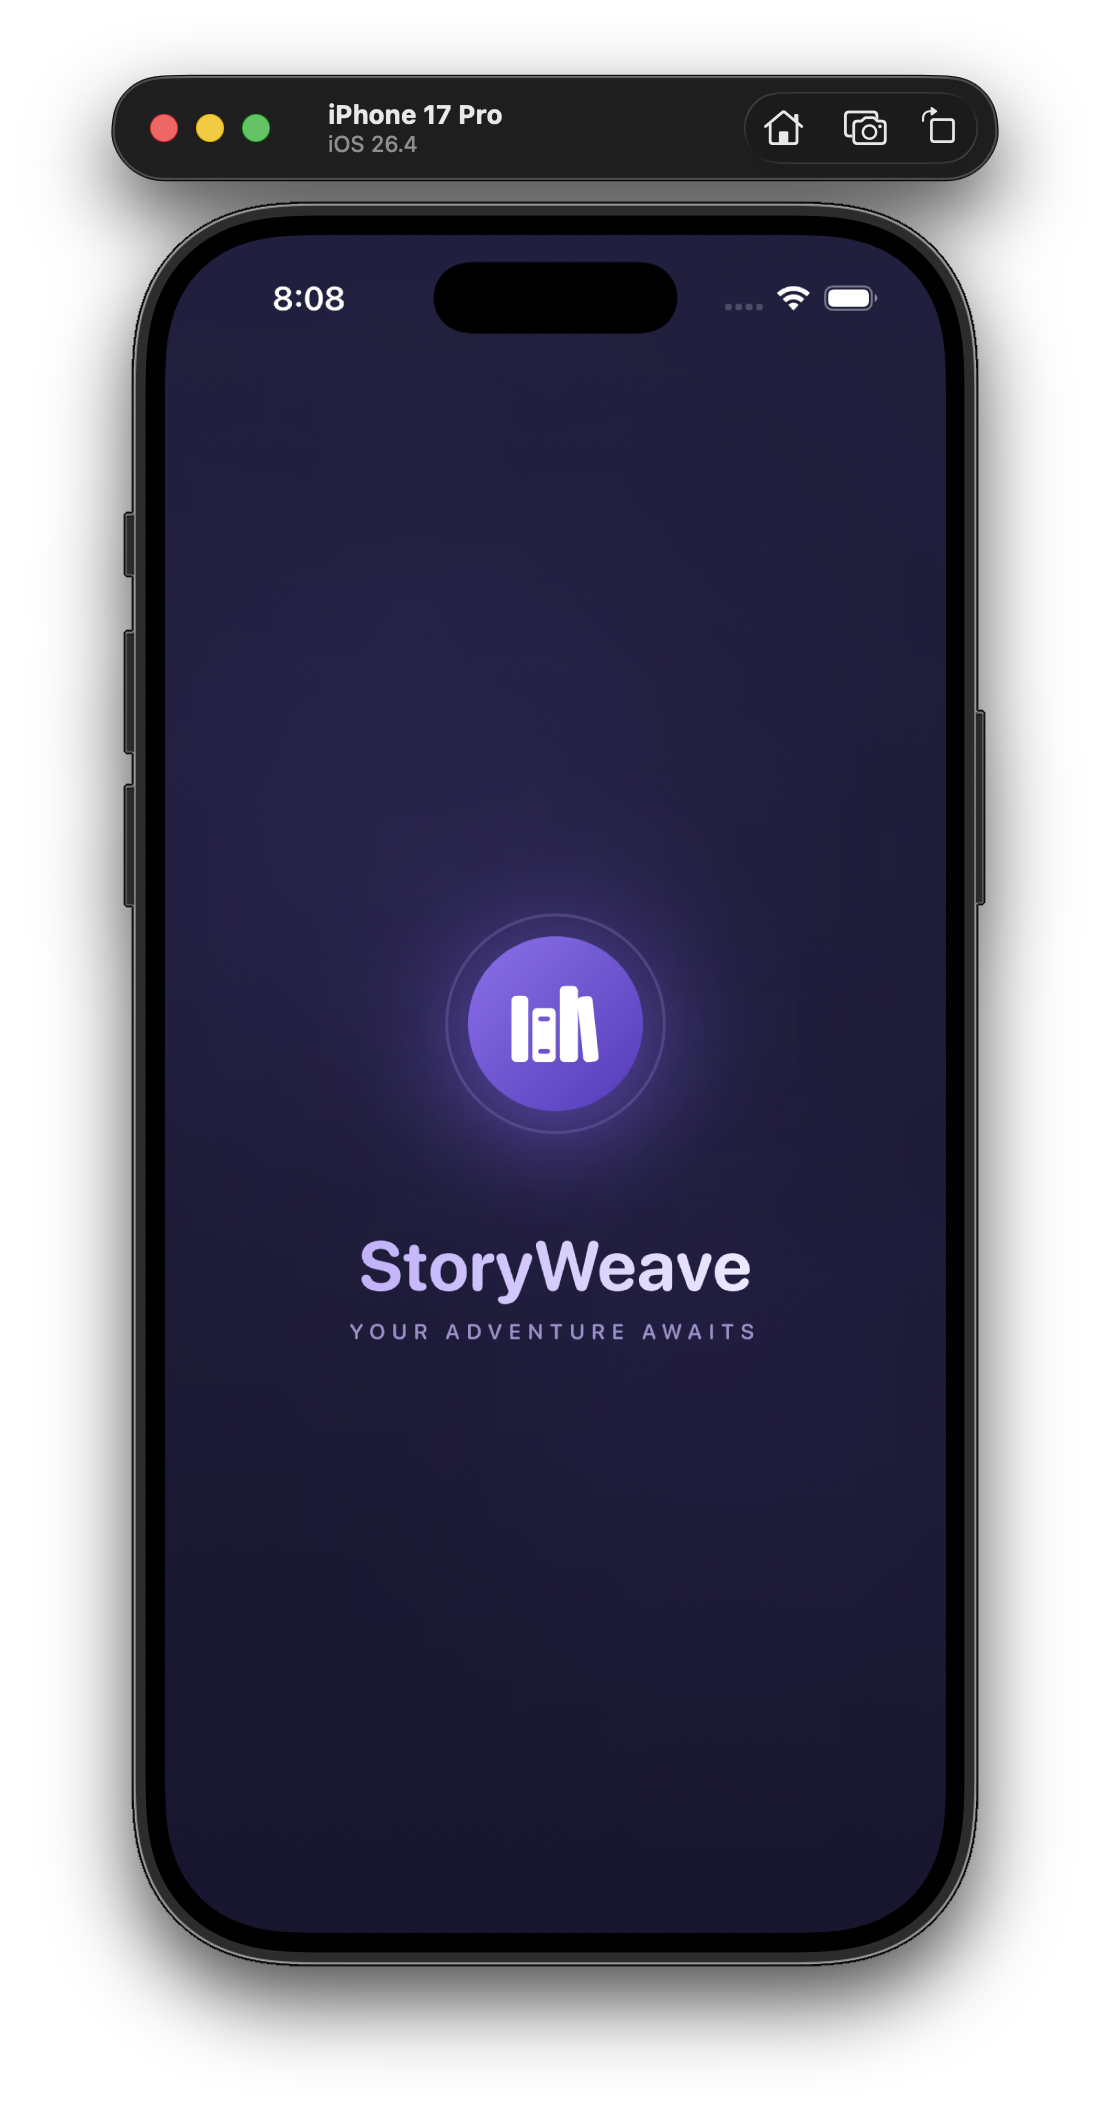
\includegraphics[width=\textwidth]{../images/0_0__splash_screen.png}
    \caption{Splash Screen}
  \end{subfigure}
  \hfill
  \begin{subfigure}[b]{0.3\textwidth}
    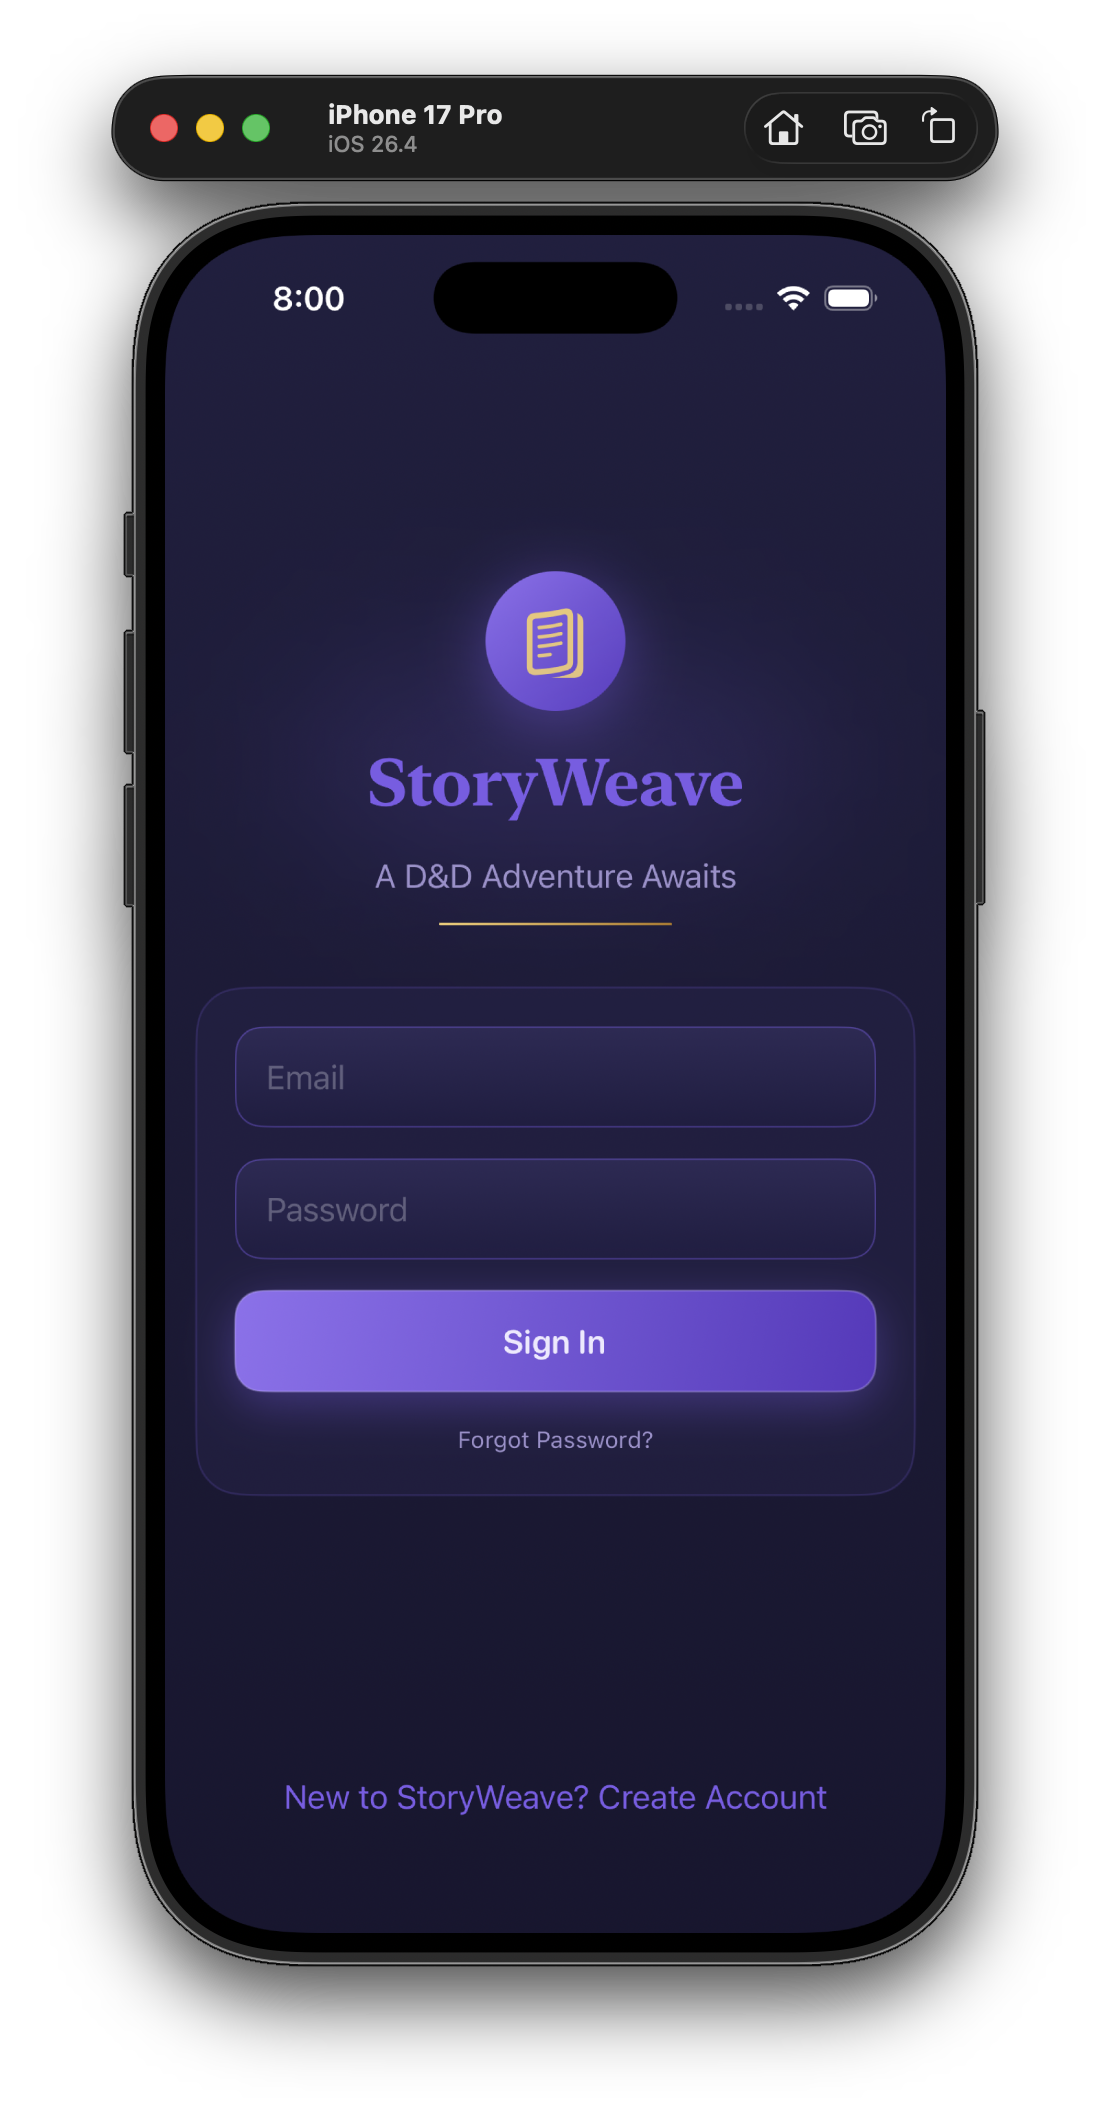
\includegraphics[width=\textwidth]{../images/1_0__sign_in.png}
    \caption{Sign In}
  \end{subfigure}
  \hfill
  \begin{subfigure}[b]{0.3\textwidth}
    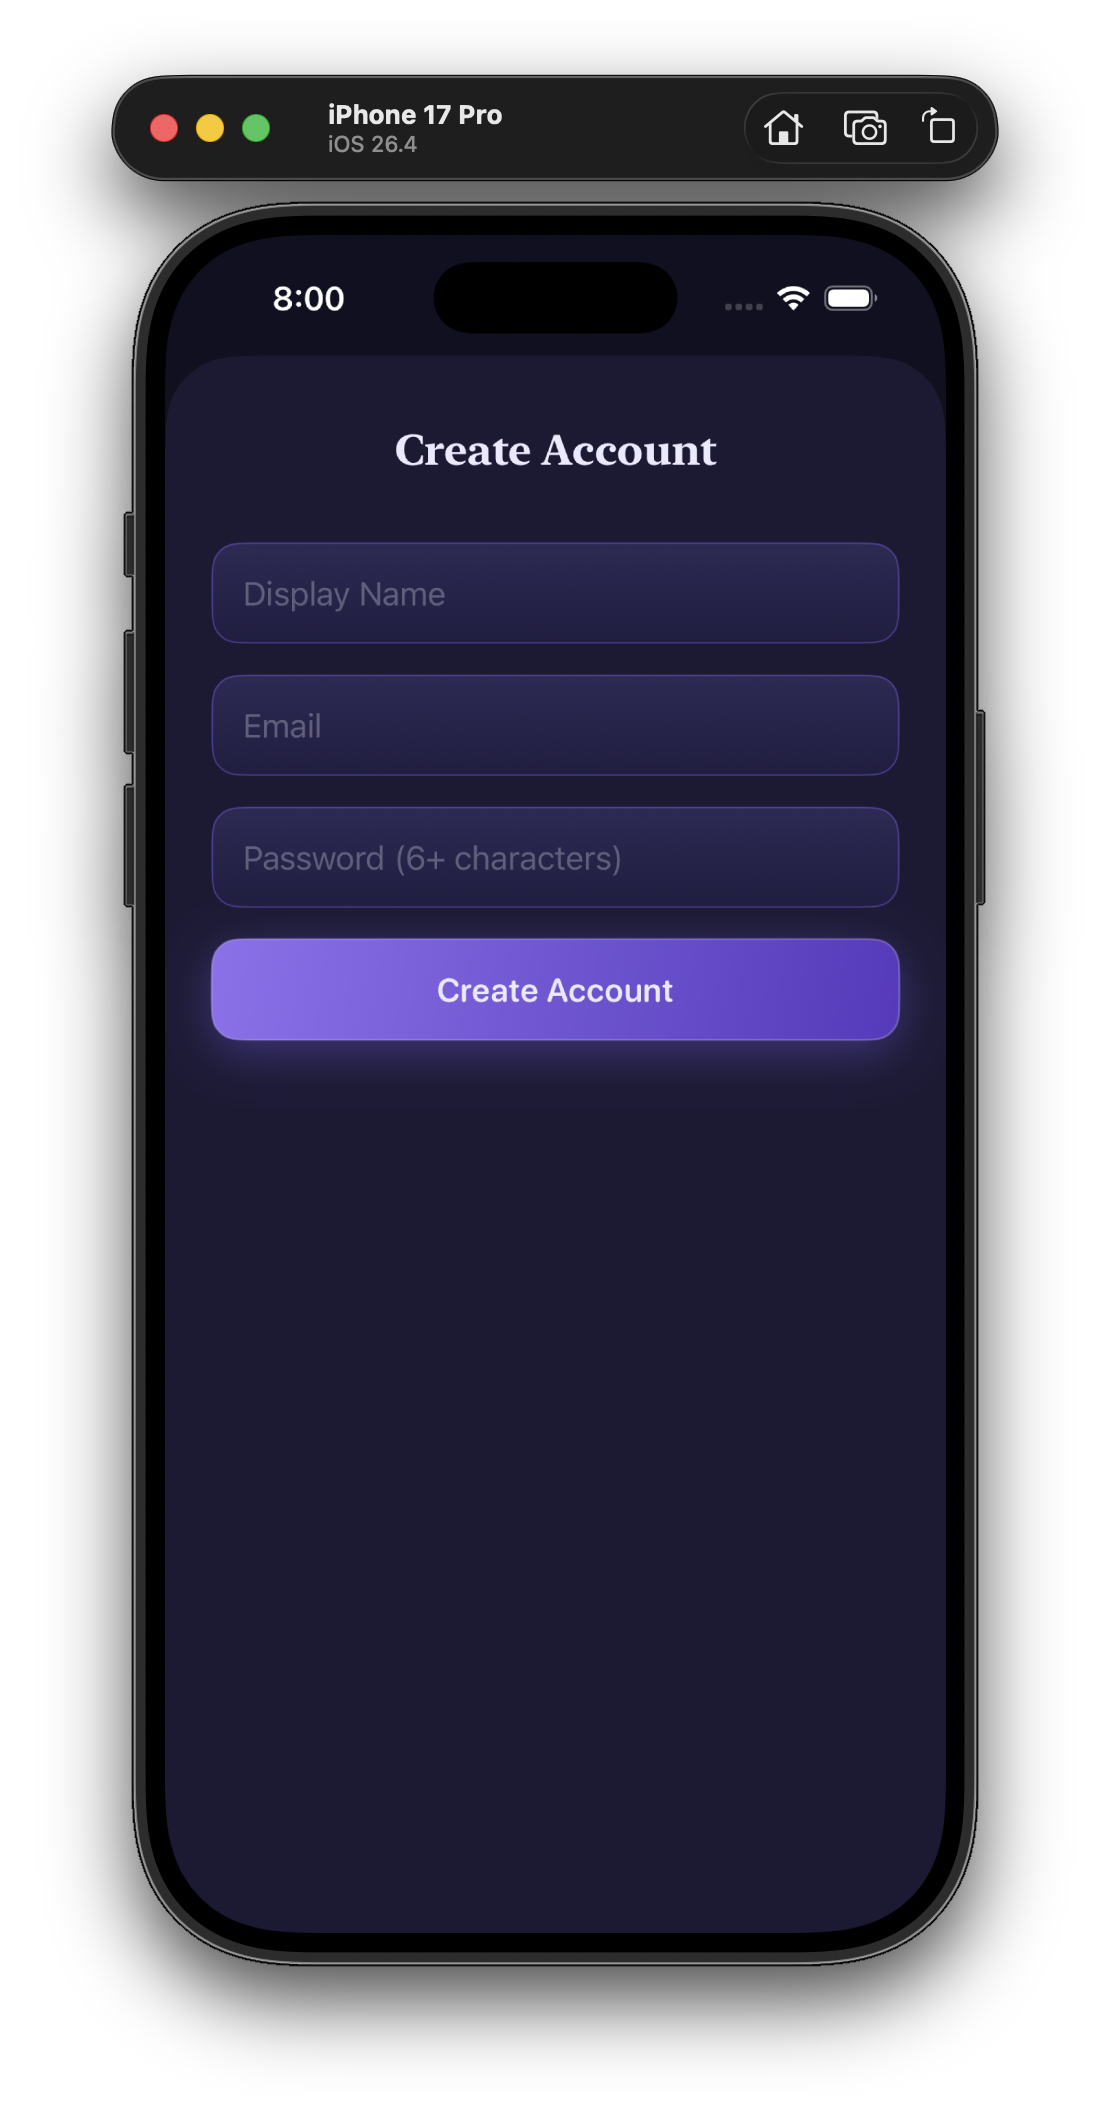
\includegraphics[width=\textwidth]{../images/1_1__sign_up.png}
    \caption{Sign Up}
  \end{subfigure}
  \caption{Authentication \& Onboarding screens}
\end{figure}

% ─────────────────────────────────────────────────────
\subsection{Profile \& Game Analytics}

\begin{itemize}[leftmargin=1.5em]
  \item Avatar upload via Cloudinary (compressed to 800 px max) with live circular preview and a ``Change Photo'' prompt.
  \item Display name badge and email shown beneath the avatar; ``Adventuring since'' join date displayed below.
  \item \textbf{Stats tab} — six analytics tiles: Combats Won, Combats Lost, Acts Done, Heroes Lost, Skill Checks attempted, and total Playtime.
  \item Combat win-rate progress bar and skill-check accuracy percentage summarise overall performance.
  \item \textbf{Inventory tab} — every item the player carries across all game runs, with description text and a quantity badge on the right.
  \item Sign Out button at the bottom of the profile screen.
\end{itemize}

\begin{figure}[H]
  \centering
  \begin{subfigure}[b]{0.3\textwidth}
    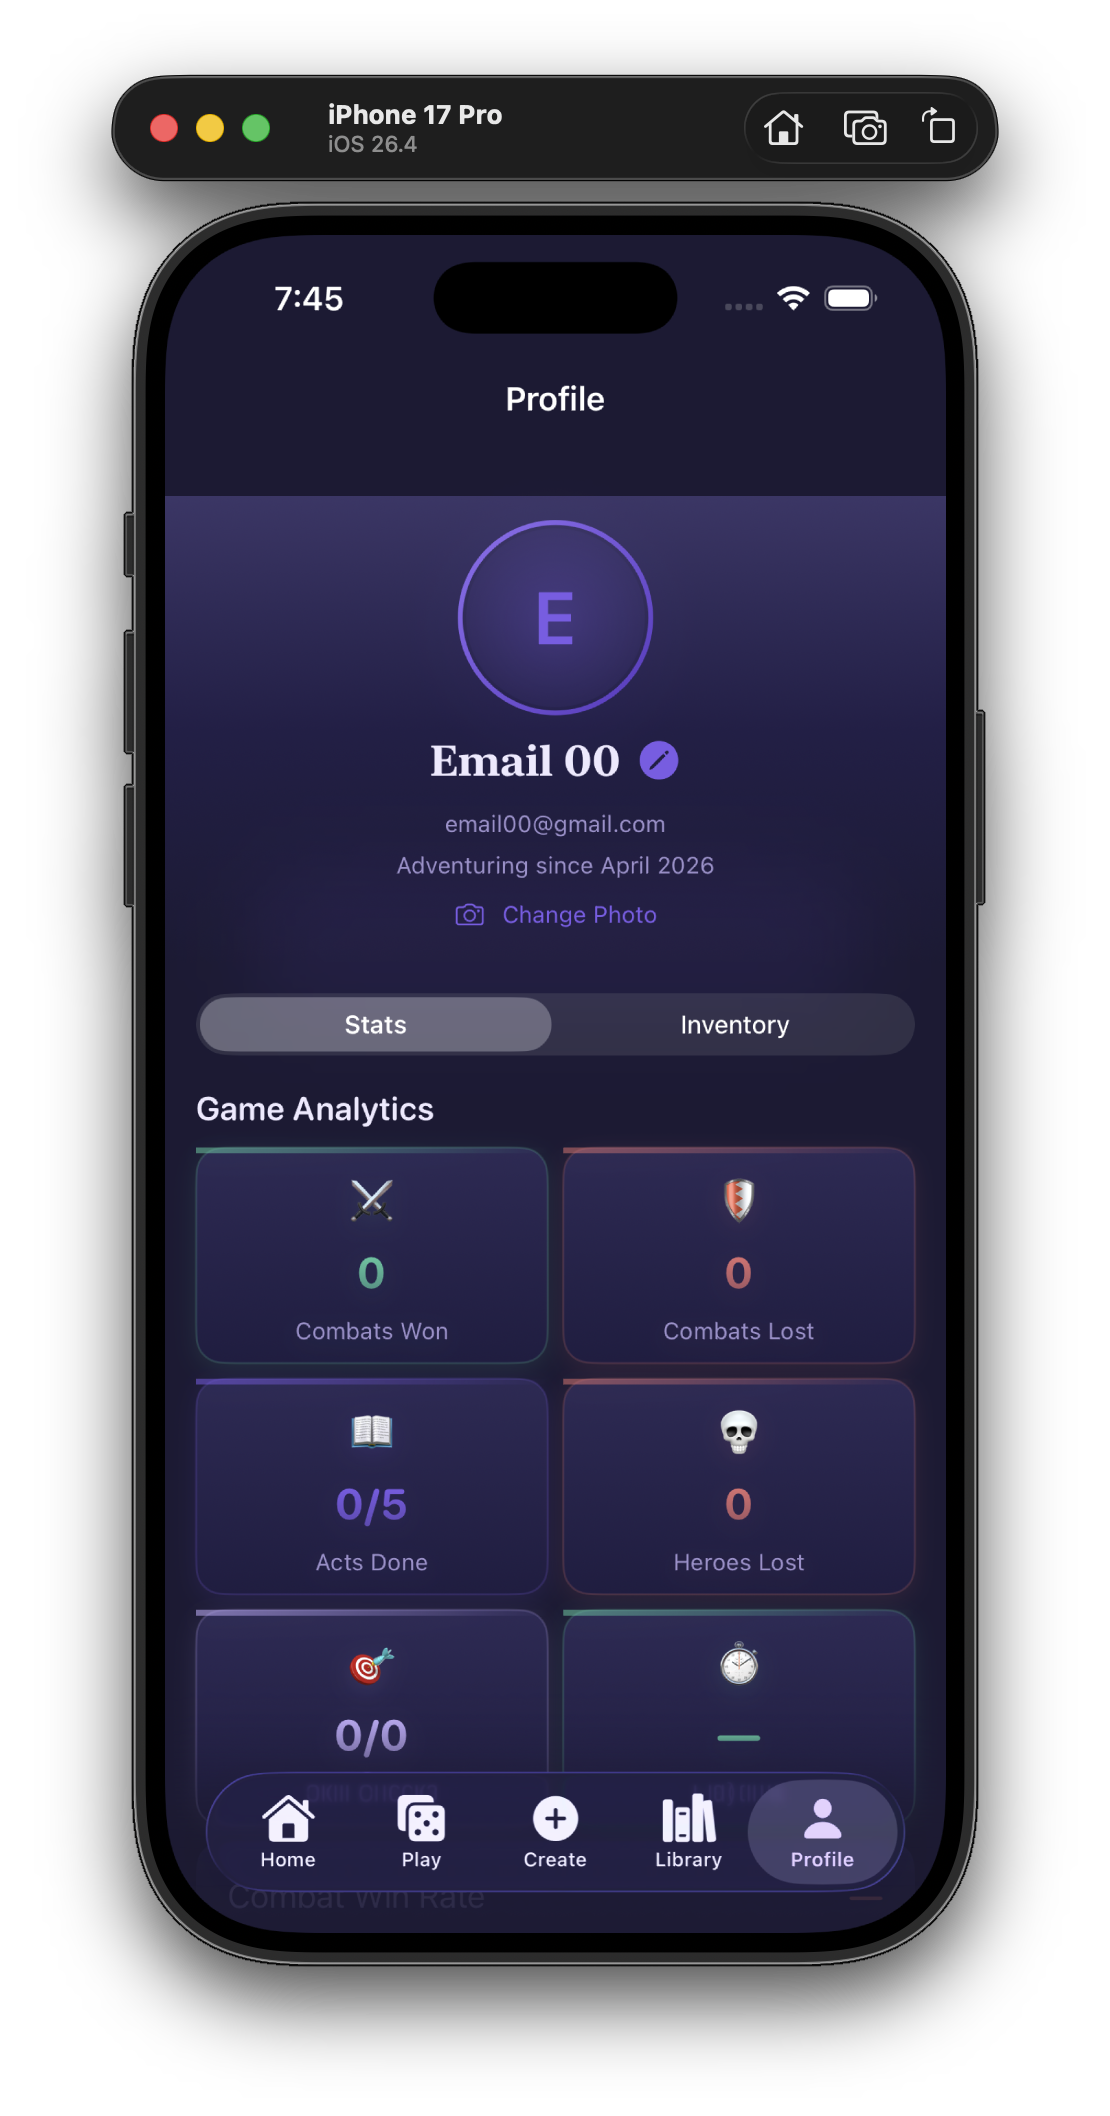
\includegraphics[width=\textwidth]{../images/2_0__profile_top.png}
    \caption{Stats (top)}
  \end{subfigure}
  \hfill
  \begin{subfigure}[b]{0.3\textwidth}
    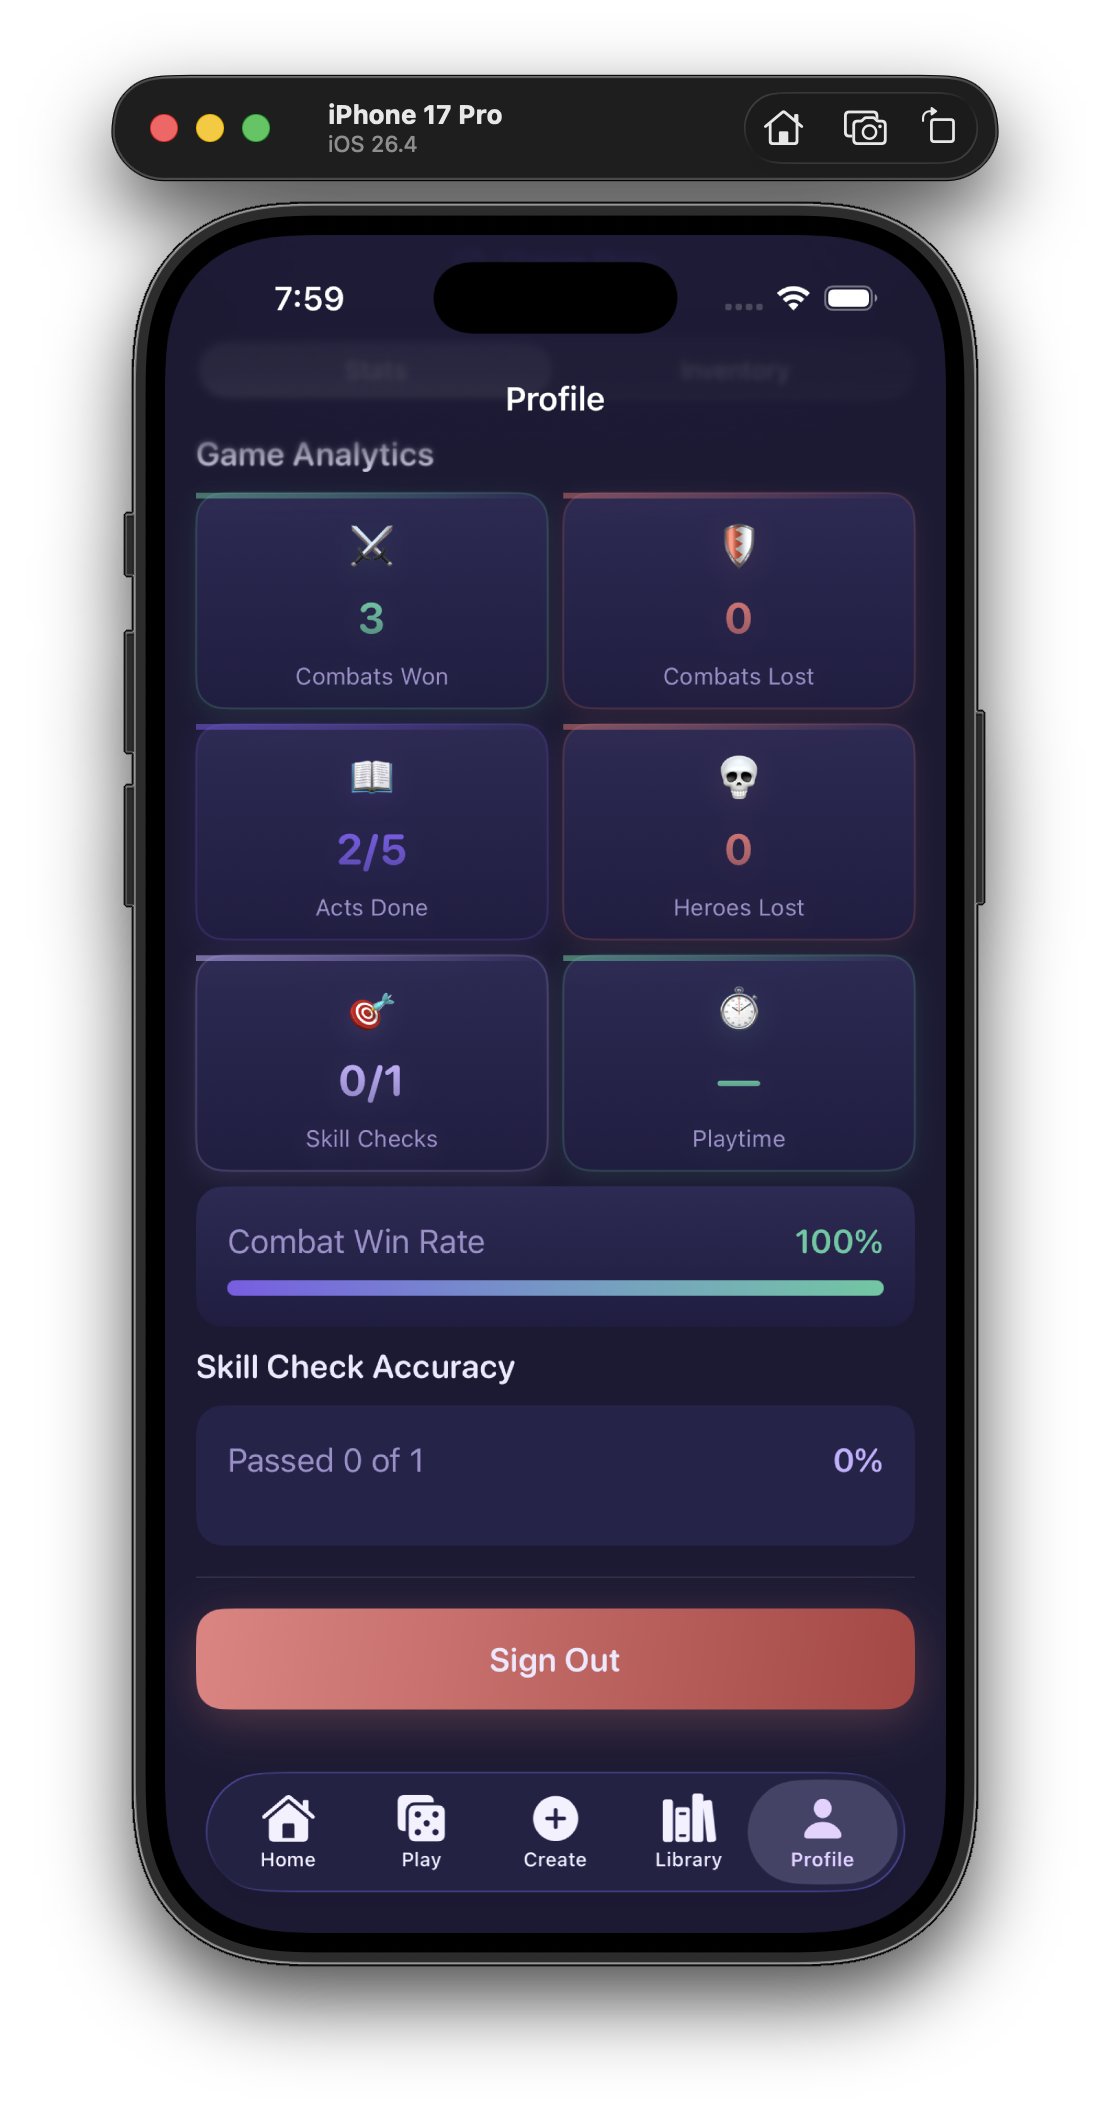
\includegraphics[width=\textwidth]{../images/2_1__profile_bottom.png}
    \caption{Analytics detail}
  \end{subfigure}
  \hfill
  \begin{subfigure}[b]{0.3\textwidth}
    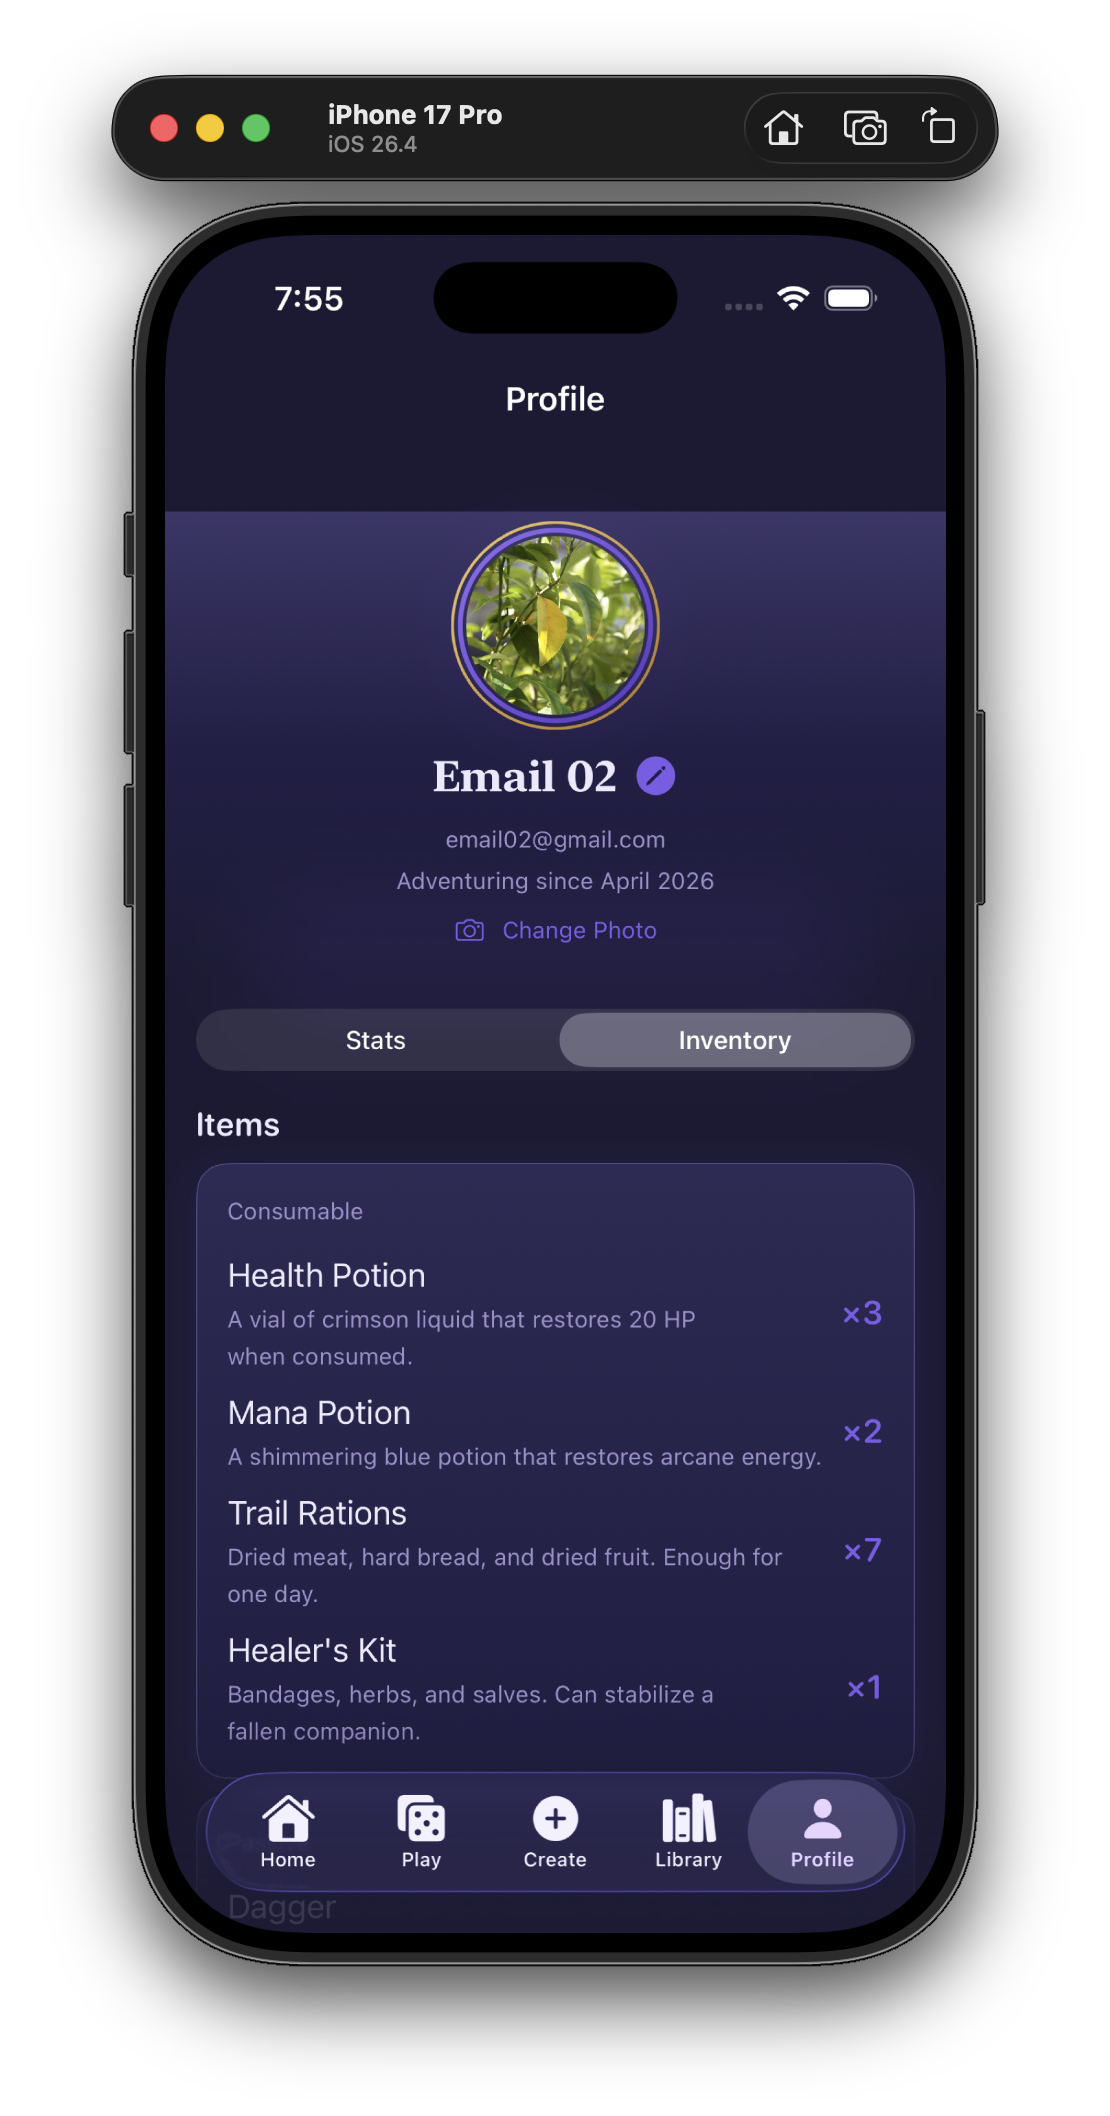
\includegraphics[width=\textwidth]{../images/2_5__inventory_top.png}
    \caption{Inventory}
  \end{subfigure}
  \caption{Profile \& Game Analytics screens}
\end{figure}

% ─────────────────────────────────────────────────────
\subsection{Library}

\begin{itemize}[leftmargin=1.5em]
  \item Searchable character browser; query matches name or archetype substring in real time.
  \item Each character row shows archetype icon, HP, ATK, and DEF at a glance.
  \item Searchable skill browser; query matches name or stat name.
  \item Each skill row shows name, description, affected-stat chip, modifier value, cooldown turns, and a colour-coded target-type badge (Enemy in red, Ally in teal, Self in muted purple).
\end{itemize}

\begin{figure}[H]
  \centering
  \begin{subfigure}[b]{0.45\textwidth}
    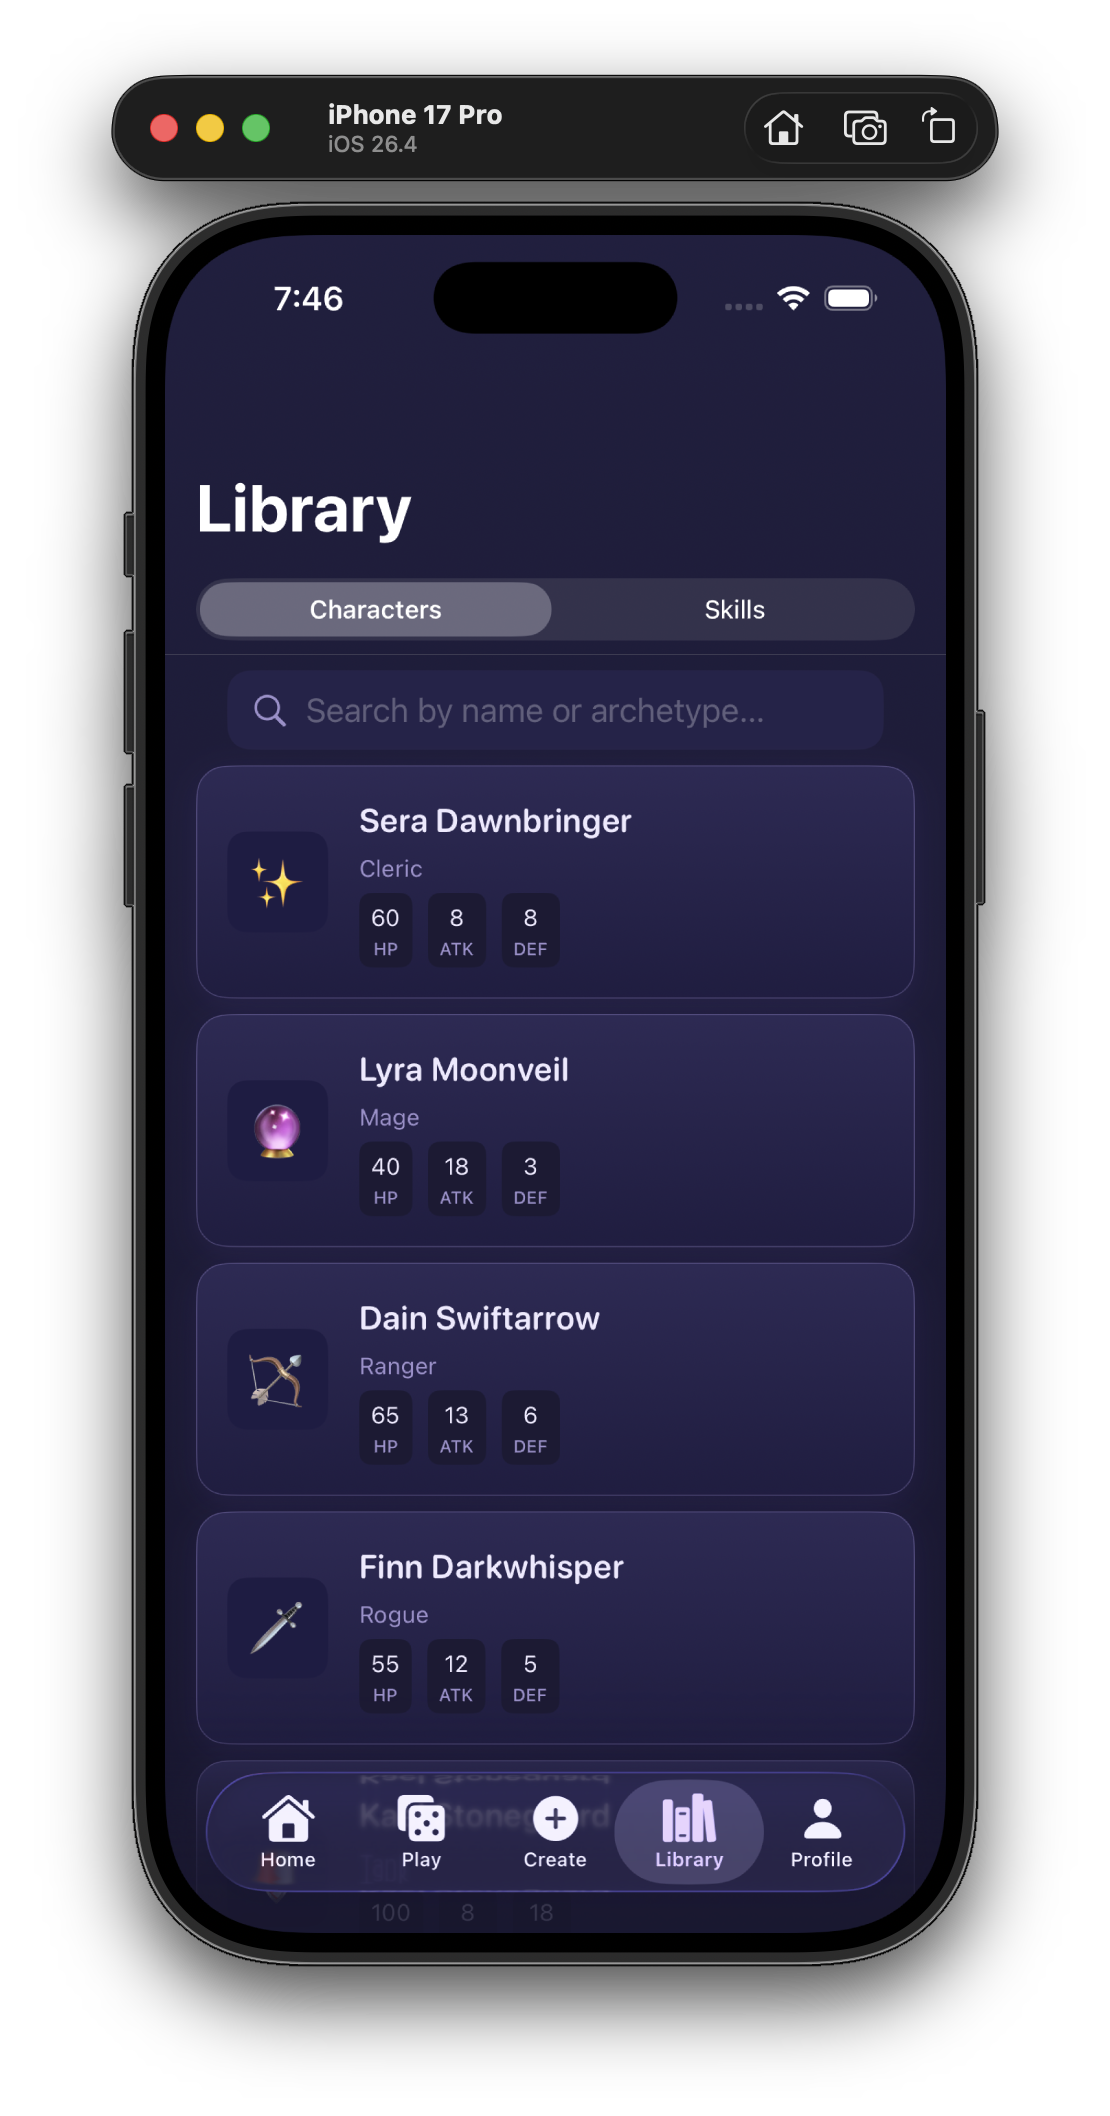
\includegraphics[width=\textwidth]{../images/3_0__library_characters.png}
    \caption{Characters}
  \end{subfigure}
  \hfill
  \begin{subfigure}[b]{0.45\textwidth}
    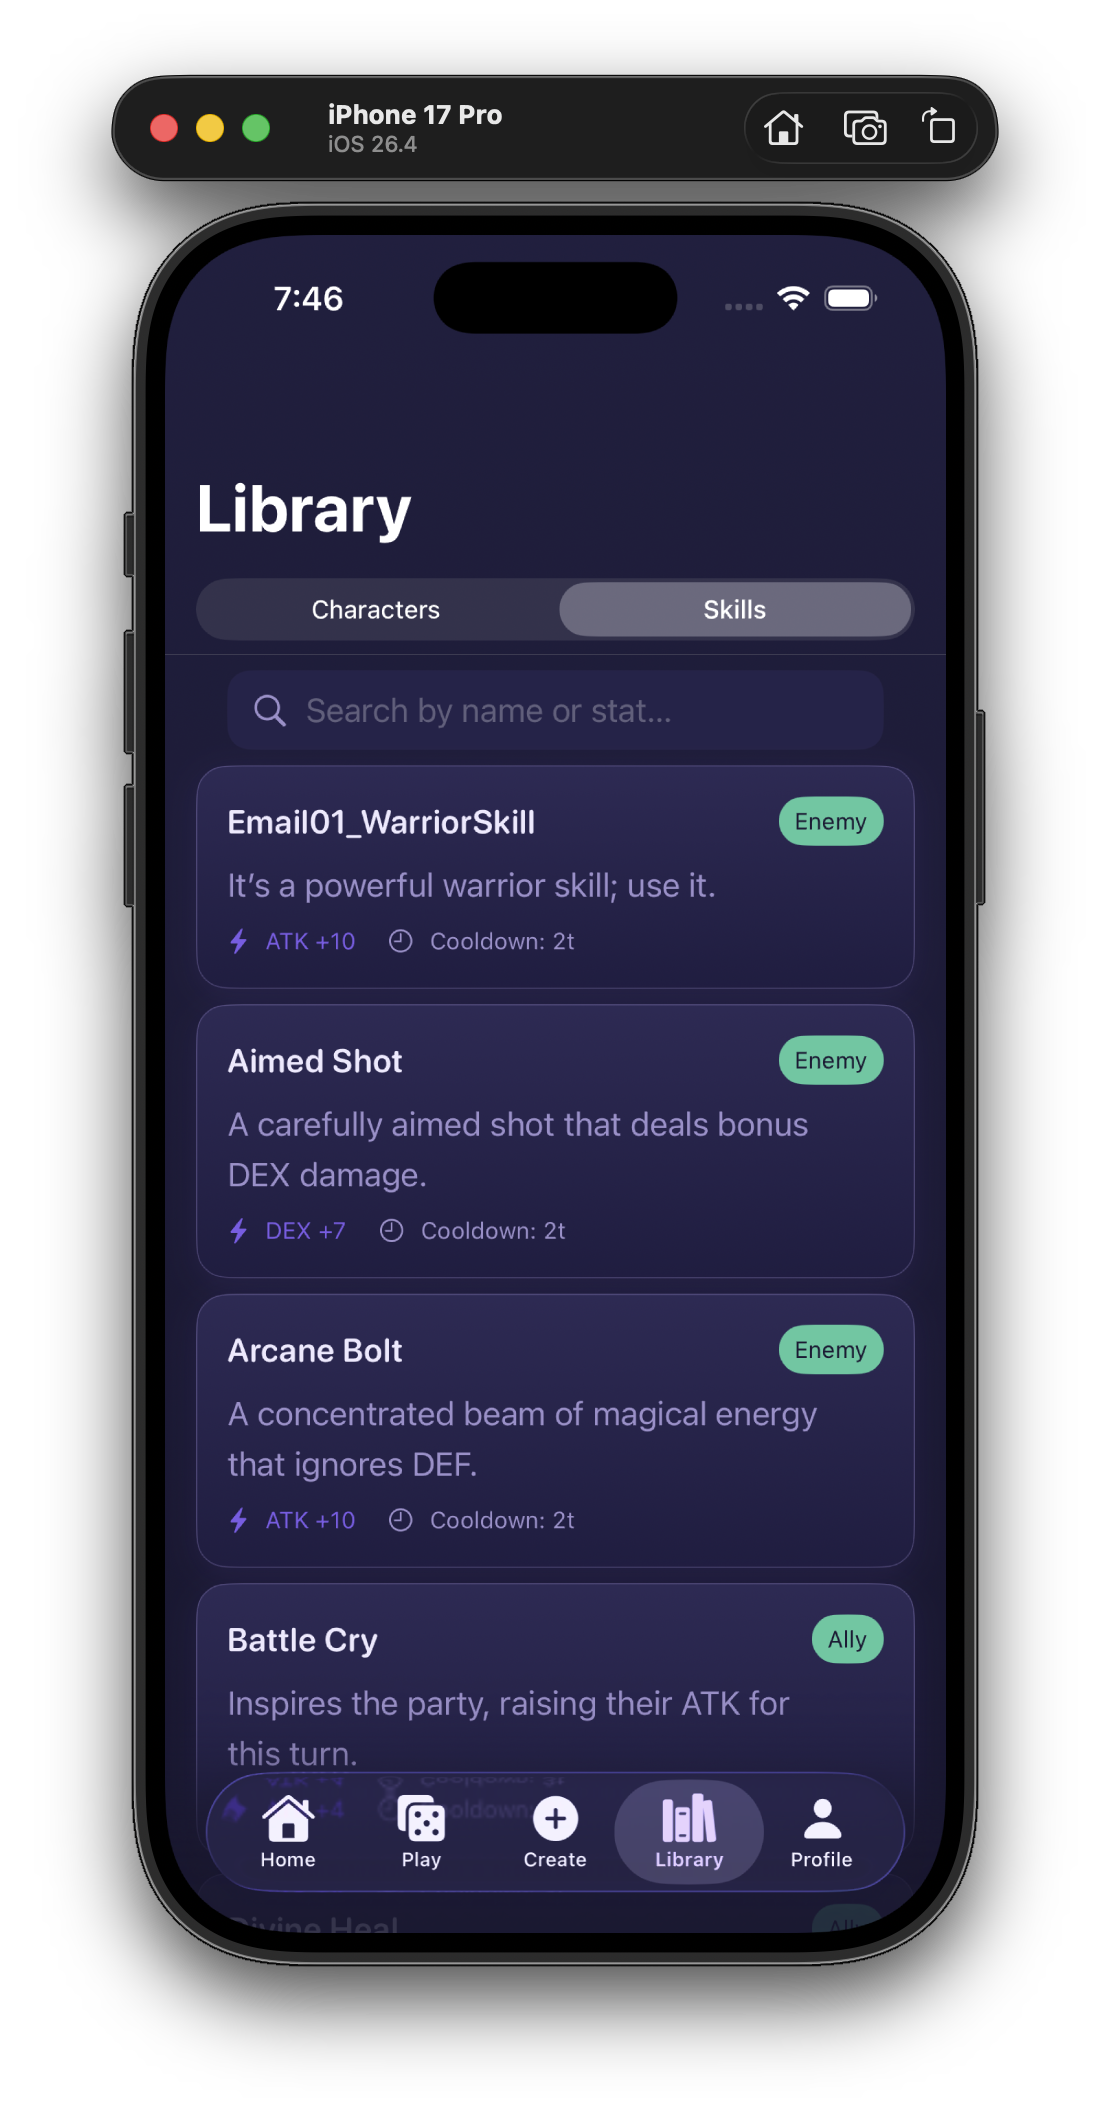
\includegraphics[width=\textwidth]{../images/3_1__library_skills.png}
    \caption{Skills}
  \end{subfigure}
  \caption{Library screen}
\end{figure}

% ─────────────────────────────────────────────────────
\subsection{Create Hub}

A central plus-tab action hub exposes four creation flows:

\begin{itemize}[leftmargin=1.5em]
  \item \textbf{Post} — rich text body, optional Cloudinary image attachment, optional character card or skill card attachment.
  \item \textbf{Character} — name field, archetype chip row (Warrior / Mage / Rogue / Cleric / Ranger / Tank), five stat sliders (Max HP, Attack, Defense, Dexterity, Intelligence), free-text lore description, and portrait upload.
  \item \textbf{Skill} — name, description, stat-affected chip row (HP / ATK / DEF / DEX / INTEL), target-type chip row (Self / Ally / Enemy / AllEnemies), modifier slider, and cooldown turns slider.
  \item \textbf{Story} — three-step wizard: (1)~Story Info (title + synopsis) $\to$ (2)~Scenes (up to 40, each with scene type, narration text, branching choices, and optional combat/skill-check config) $\to$ (3)~Review \& Publish.
\end{itemize}

\begin{figure}[H]
  \centering
  \begin{subfigure}[b]{0.22\textwidth}
    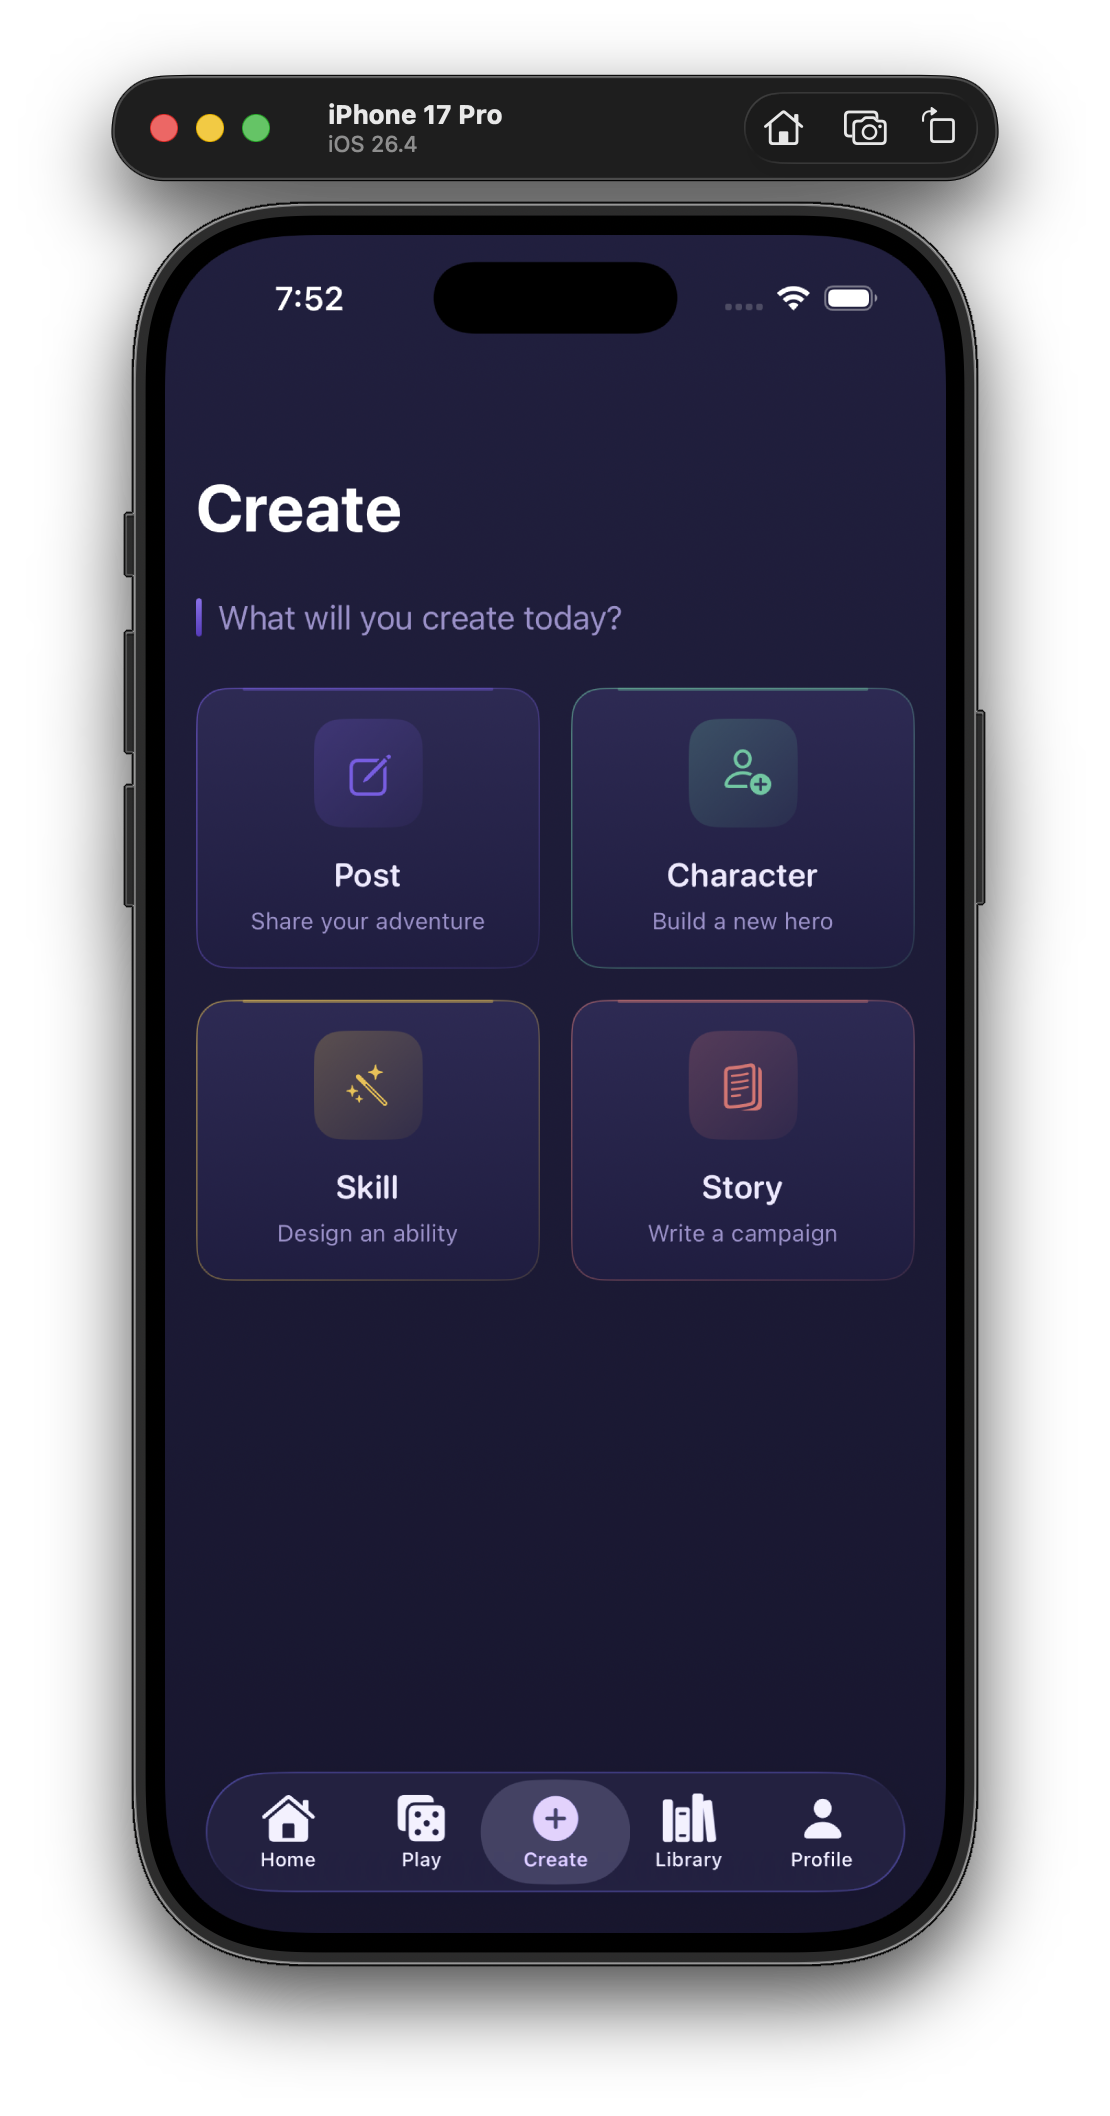
\includegraphics[width=\textwidth]{../images/4_0__create_things.png}
    \caption{Hub}
  \end{subfigure}
  \hfill
  \begin{subfigure}[b]{0.22\textwidth}
    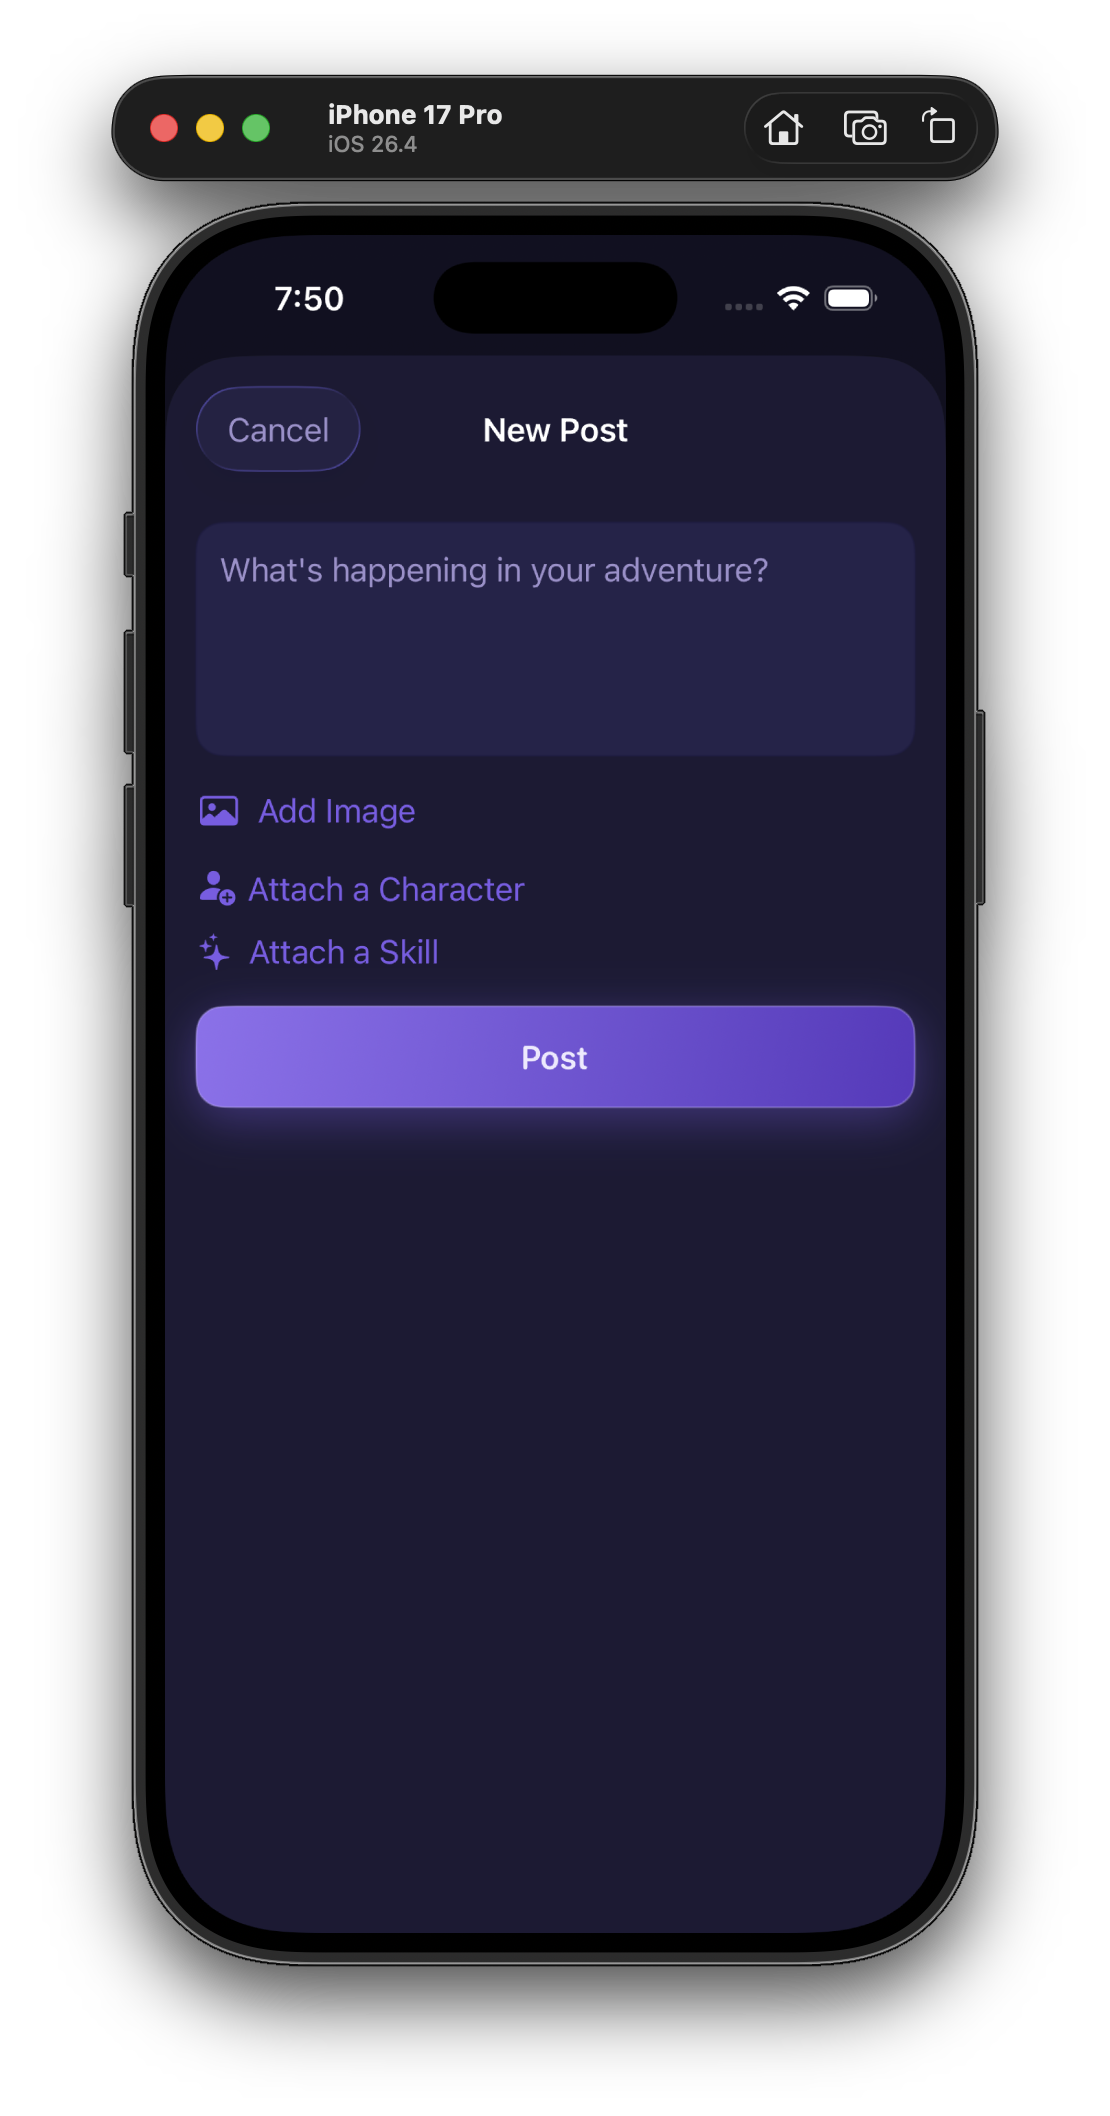
\includegraphics[width=\textwidth]{../images/4_1__create_new_post.png}
    \caption{New Post}
  \end{subfigure}
  \hfill
  \begin{subfigure}[b]{0.22\textwidth}
    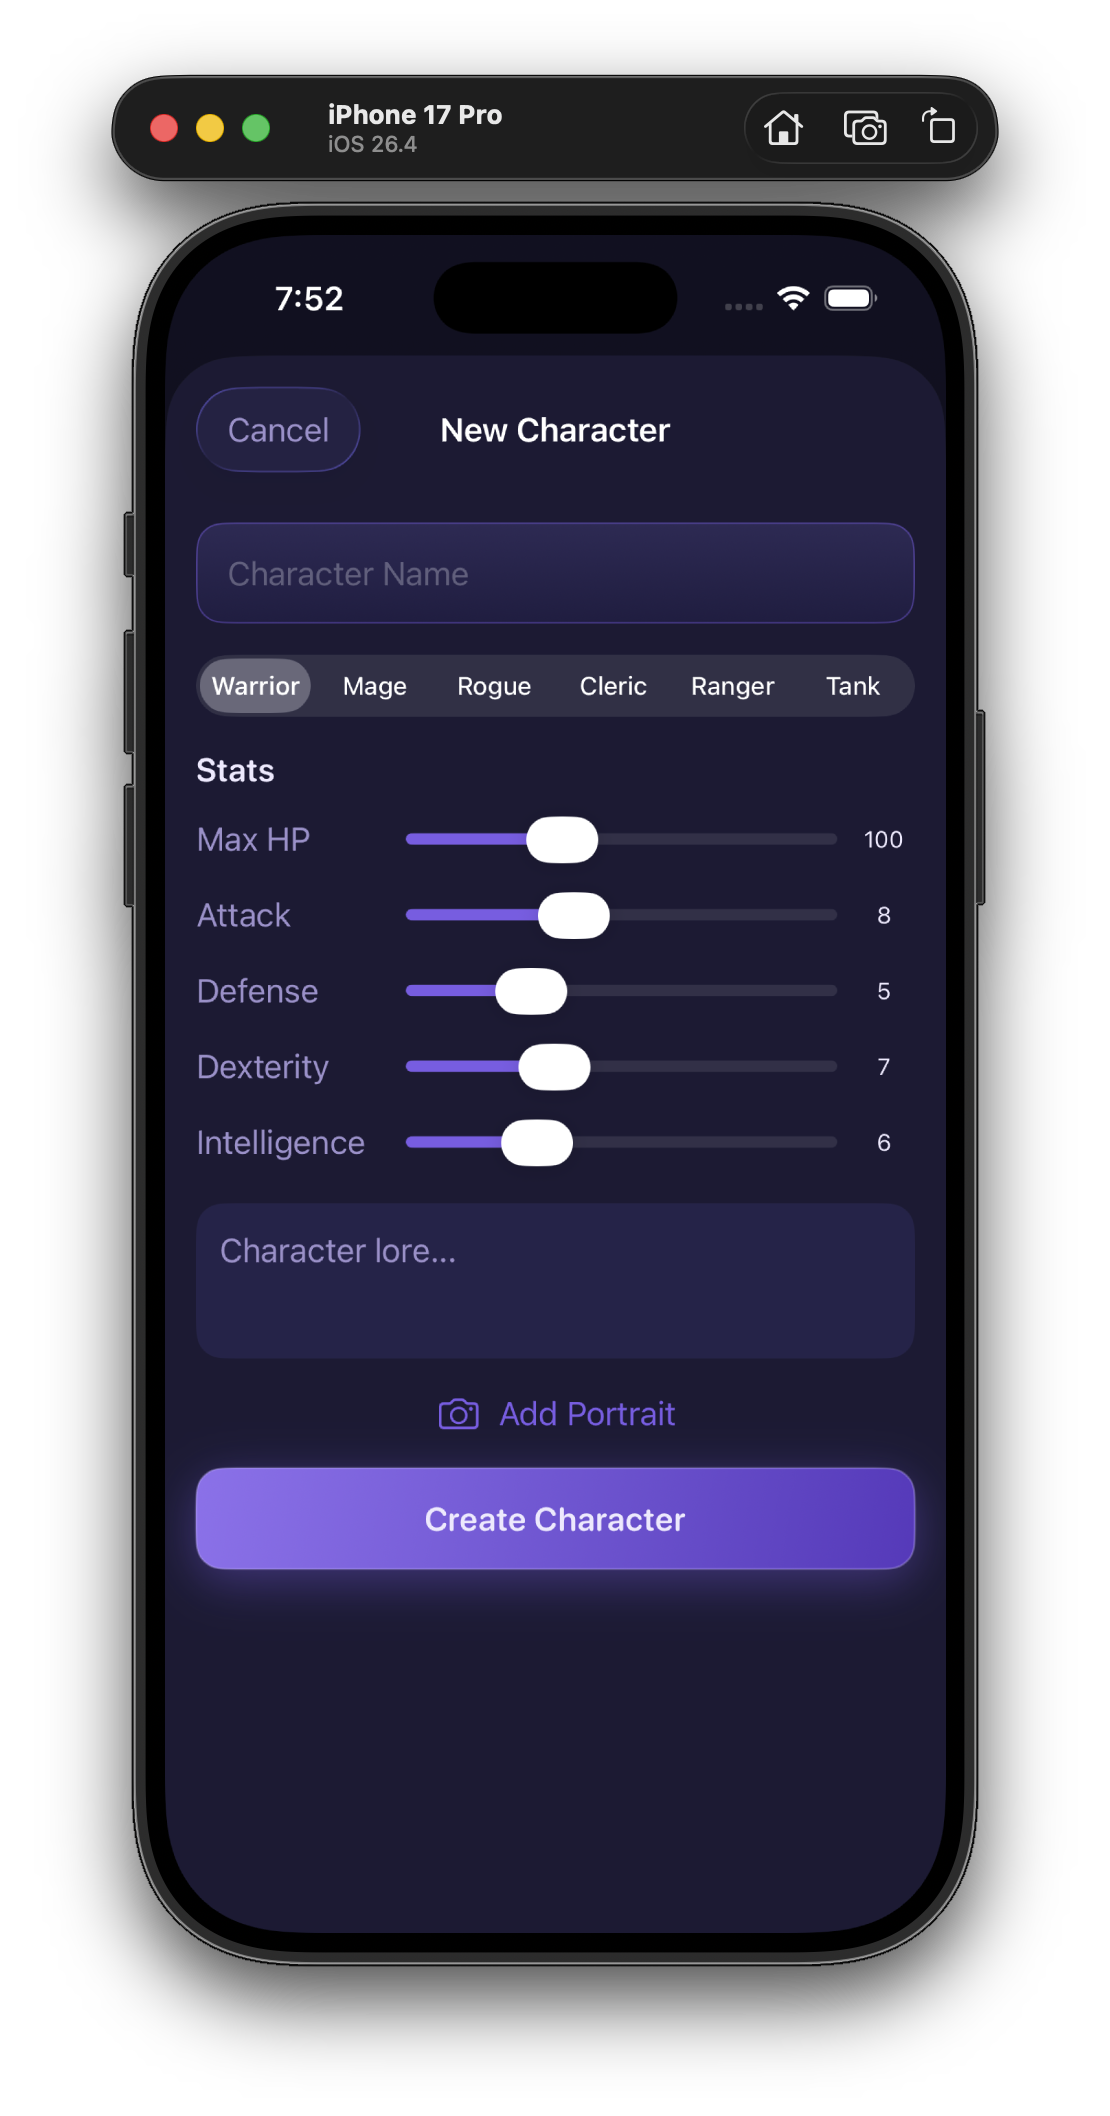
\includegraphics[width=\textwidth]{../images/4_2__create_new_character.png}
    \caption{New Character}
  \end{subfigure}
  \hfill
  \begin{subfigure}[b]{0.22\textwidth}
    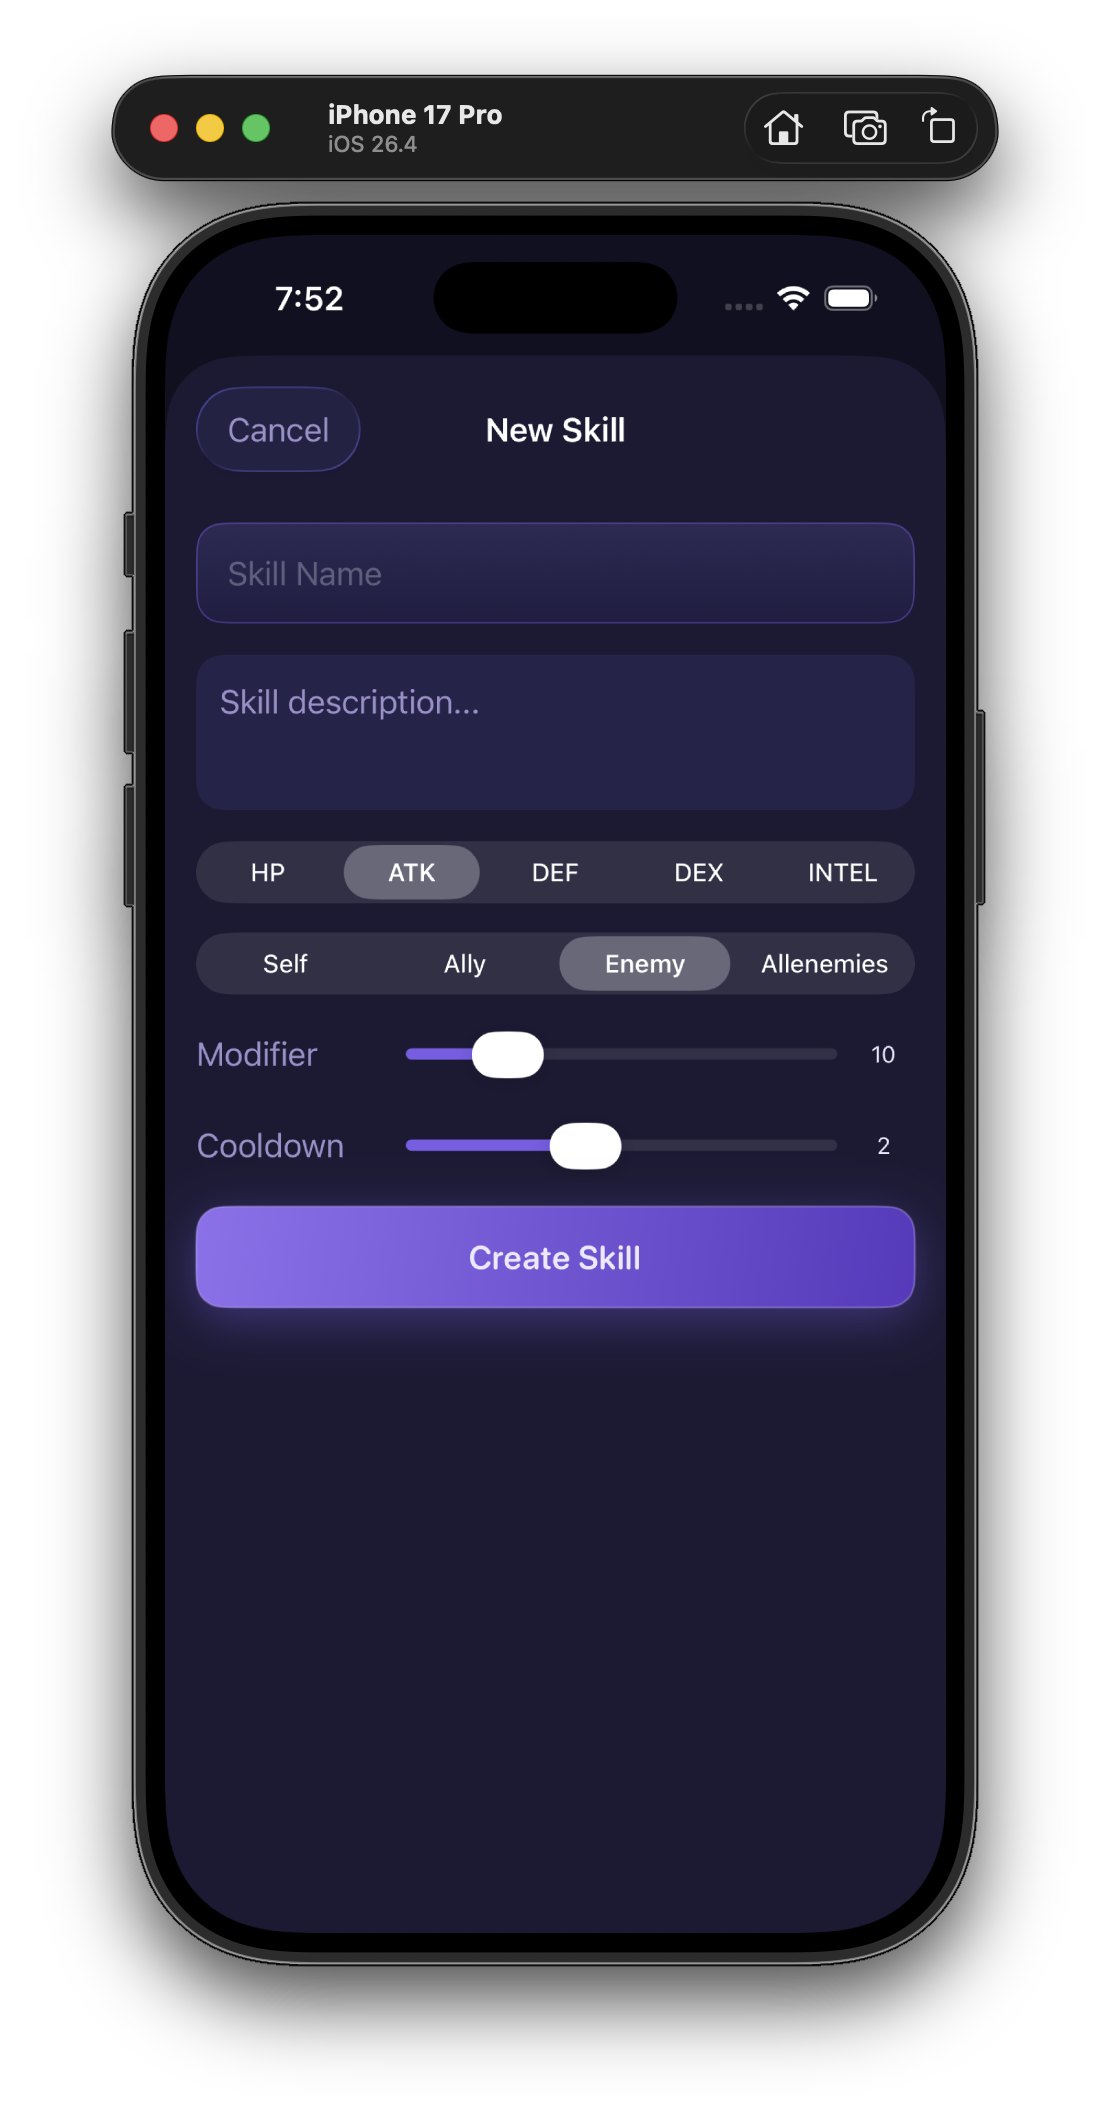
\includegraphics[width=\textwidth]{../images/4_3__create_new_skill.png}
    \caption{New Skill}
  \end{subfigure}
  \caption{Create Hub flows}
\end{figure}

\begin{figure}[H]
  \centering
  \begin{subfigure}[b]{0.35\textwidth}
    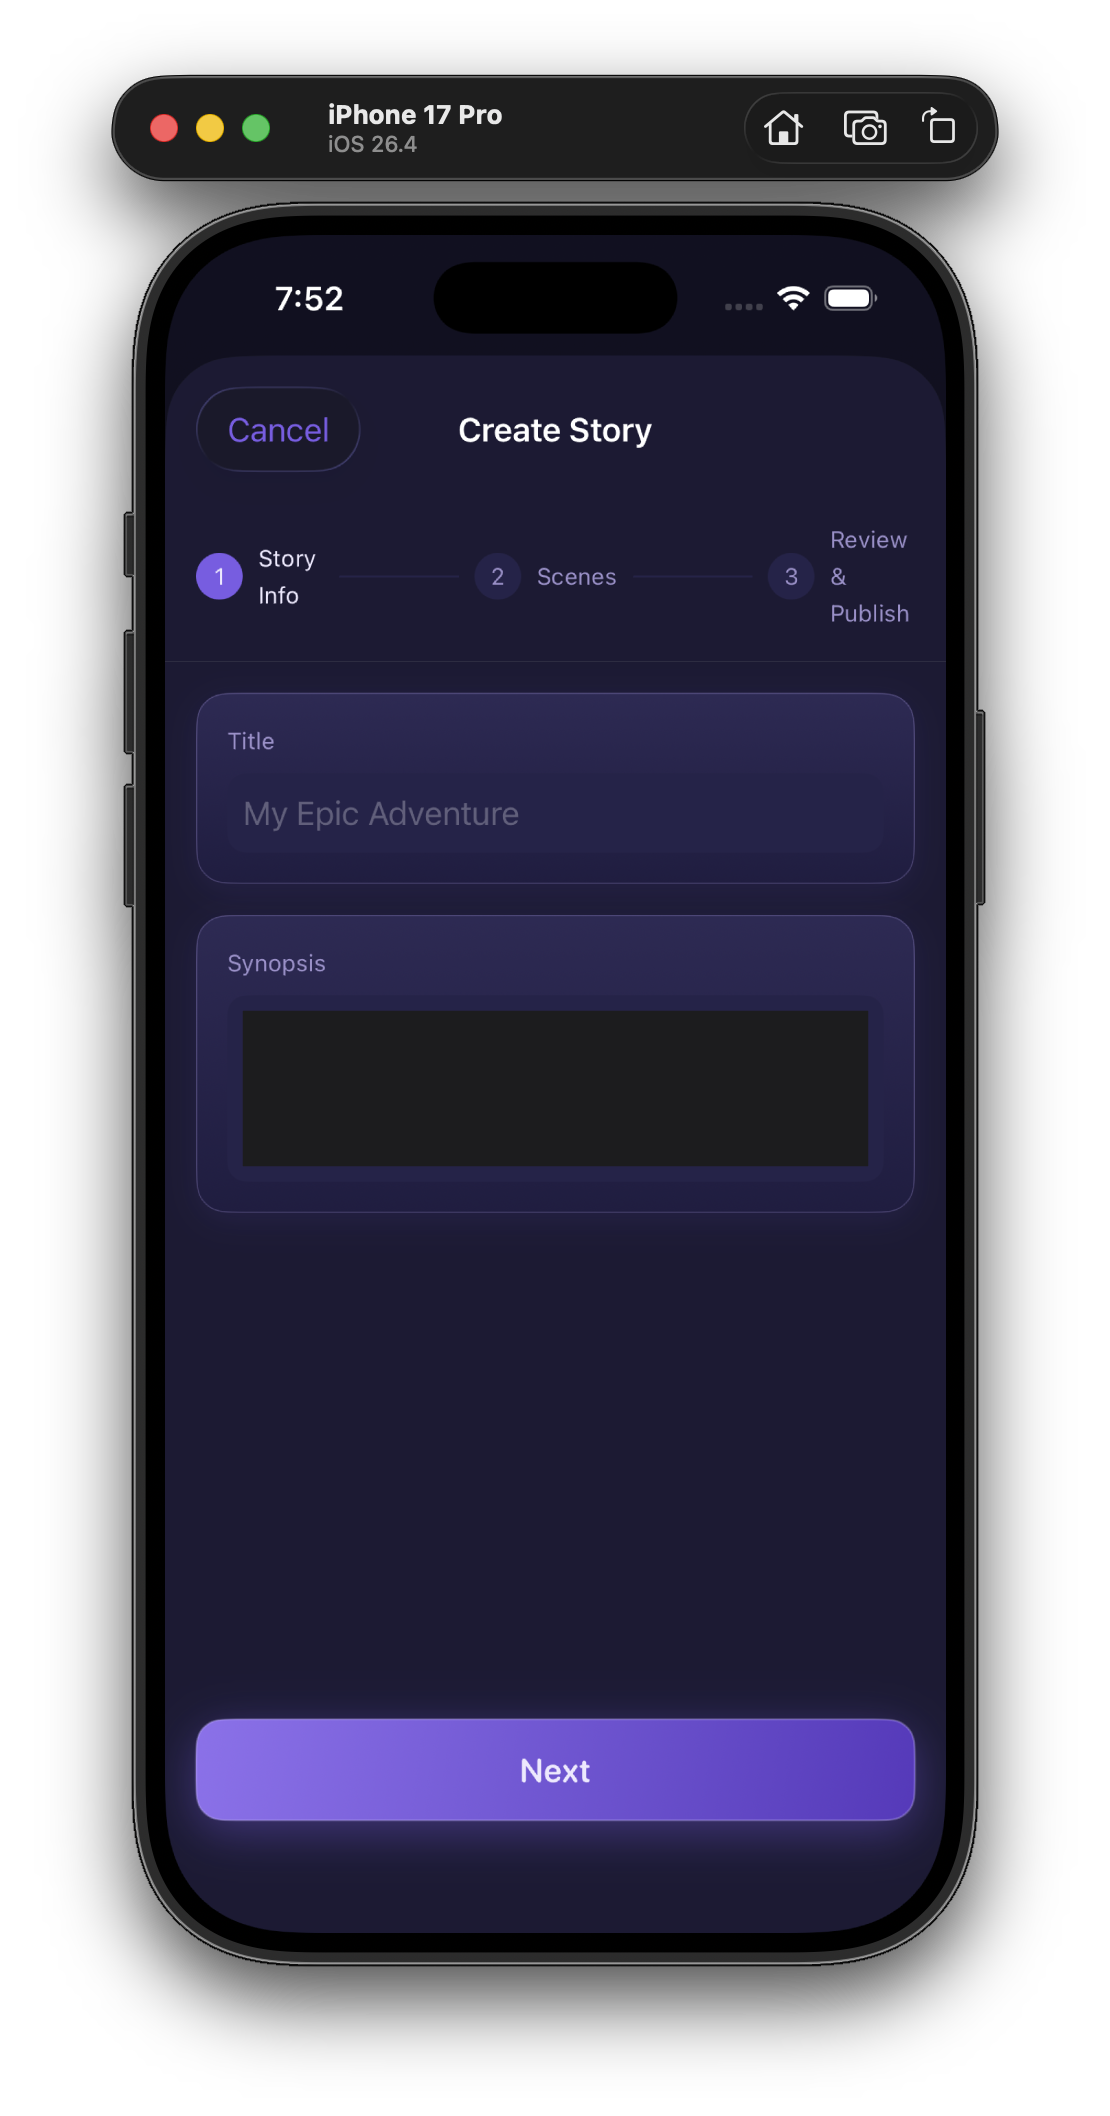
\includegraphics[width=\textwidth]{../images/4_4__create_story.png}
    \caption{Story Wizard}
  \end{subfigure}
  \caption{Create Story wizard — Step 1: Story Info}
\end{figure}

% ─────────────────────────────────────────────────────
\subsection{Community Feed}

\begin{itemize}[leftmargin=1.5em]
  \item Global social feed aggregates all users' posts in reverse-chronological order with a real-time Firestore snapshot listener.
  \item Post cards show author avatar initial, display name, relative timestamp, body text, and an inline character or skill card preview where attached.
  \item Full-screen post detail view shows emoji reaction row (\texttt{❤️ 😂 😮 👏}), like count, and a scrollable comment section.
  \item Comments support one level of threaded replies; reply indentation is shown inline.
  \item Post authors can edit or delete their own posts via an overflow menu (\texttt{⋯}).
\end{itemize}

\begin{figure}[H]
  \centering
  \begin{subfigure}[b]{0.3\textwidth}
    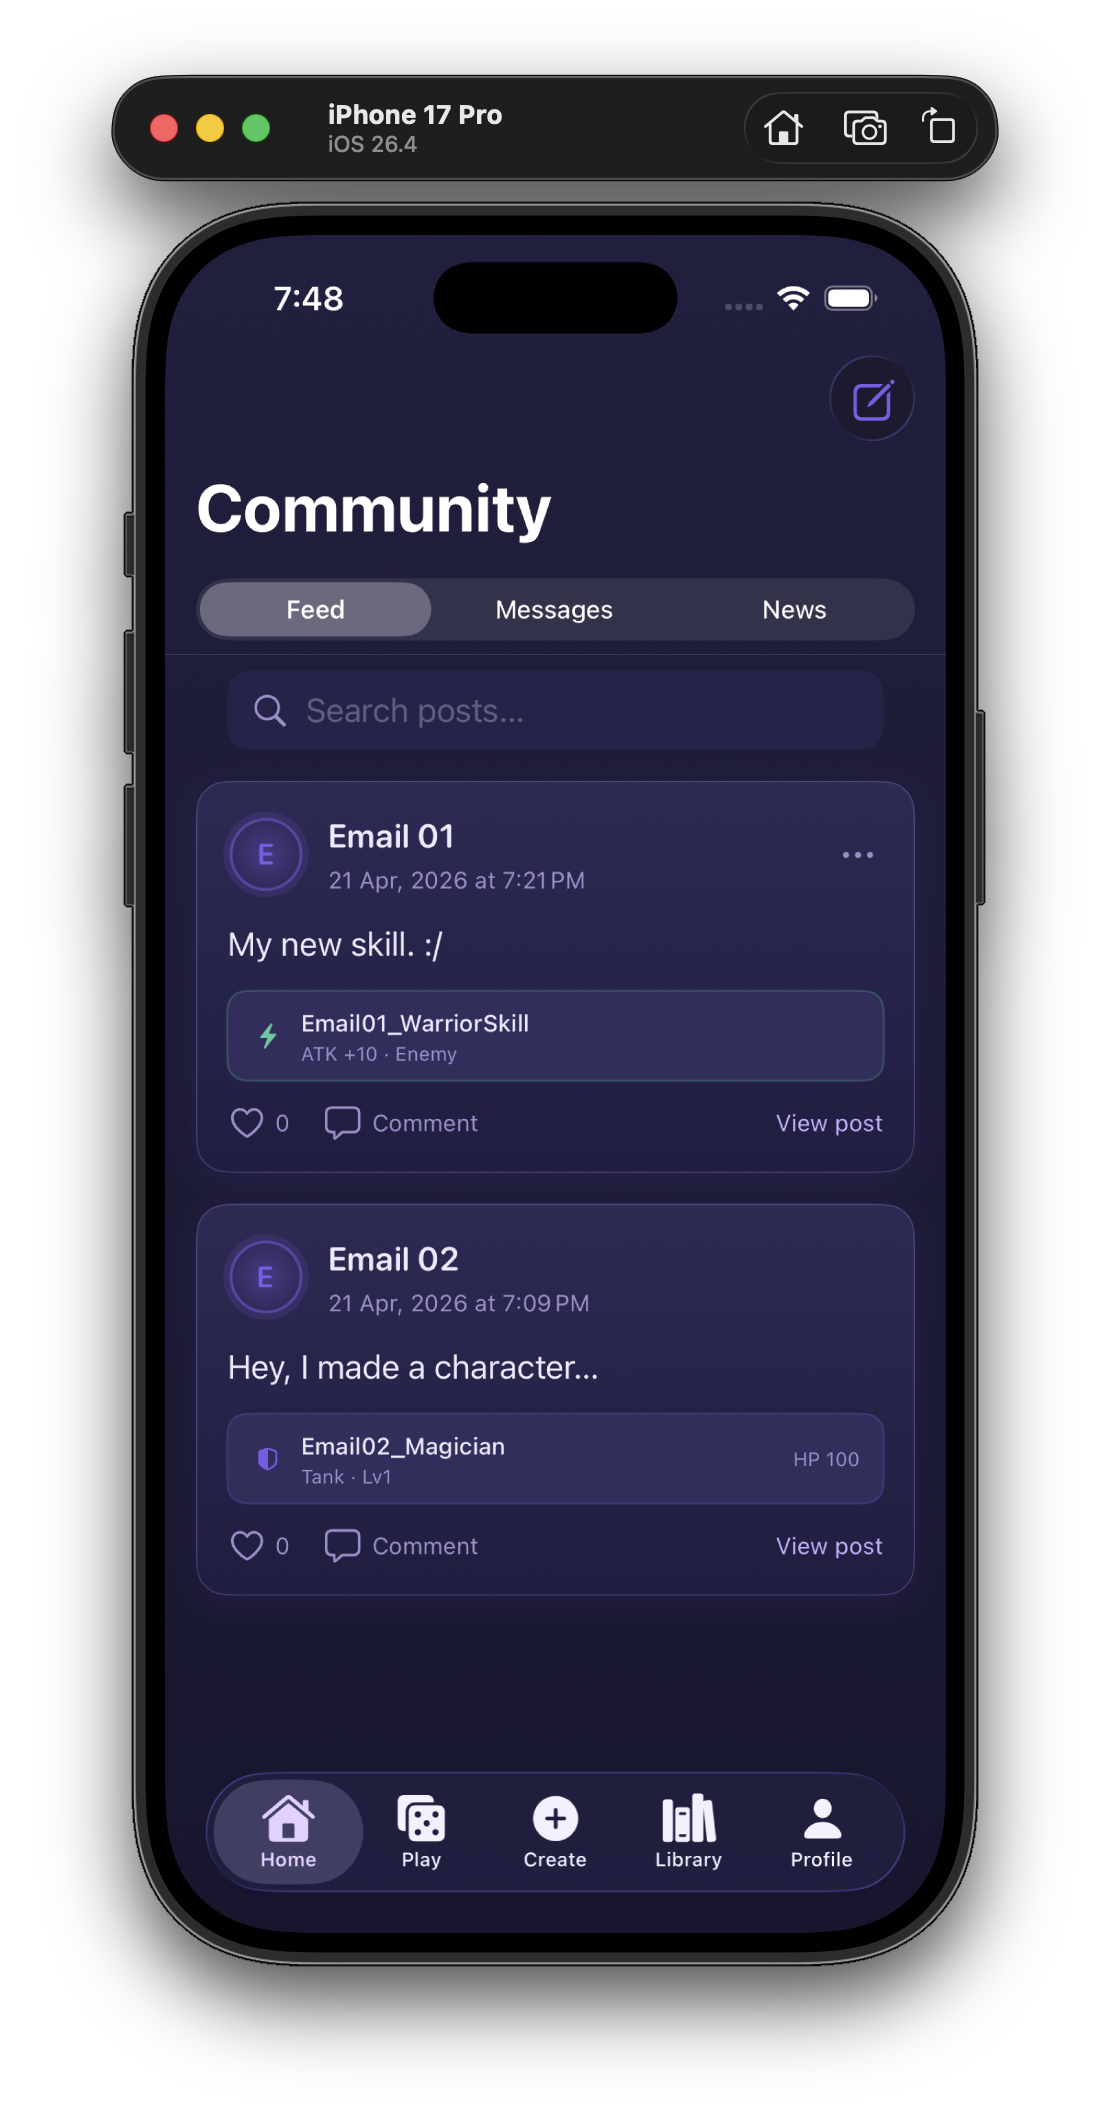
\includegraphics[width=\textwidth]{../images/5_0__feed_posts.png}
    \caption{Feed}
  \end{subfigure}
  \hfill
  \begin{subfigure}[b]{0.3\textwidth}
    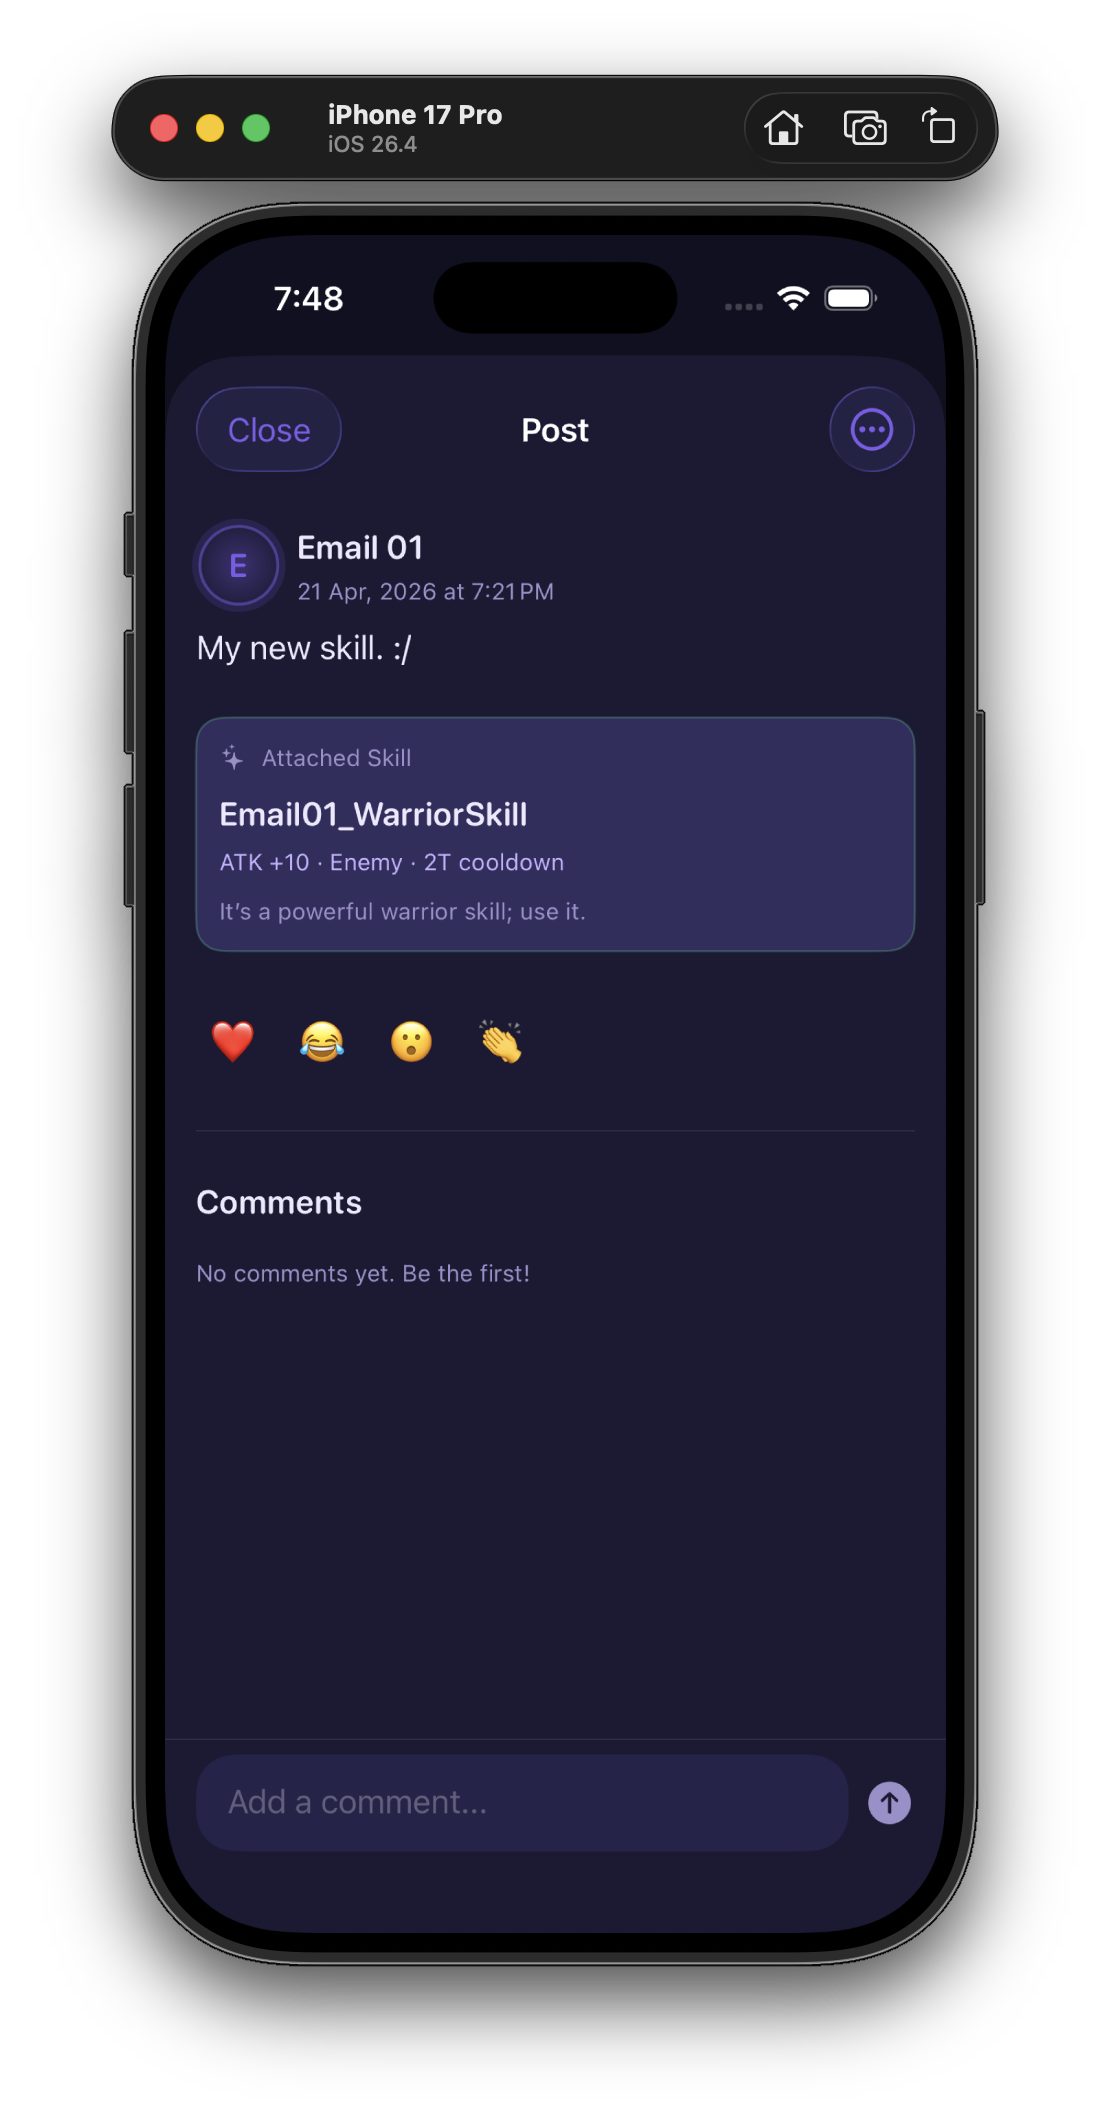
\includegraphics[width=\textwidth]{../images/5_1__post_details.png}
    \caption{Post Detail}
  \end{subfigure}
  \hfill
  \begin{subfigure}[b]{0.3\textwidth}
    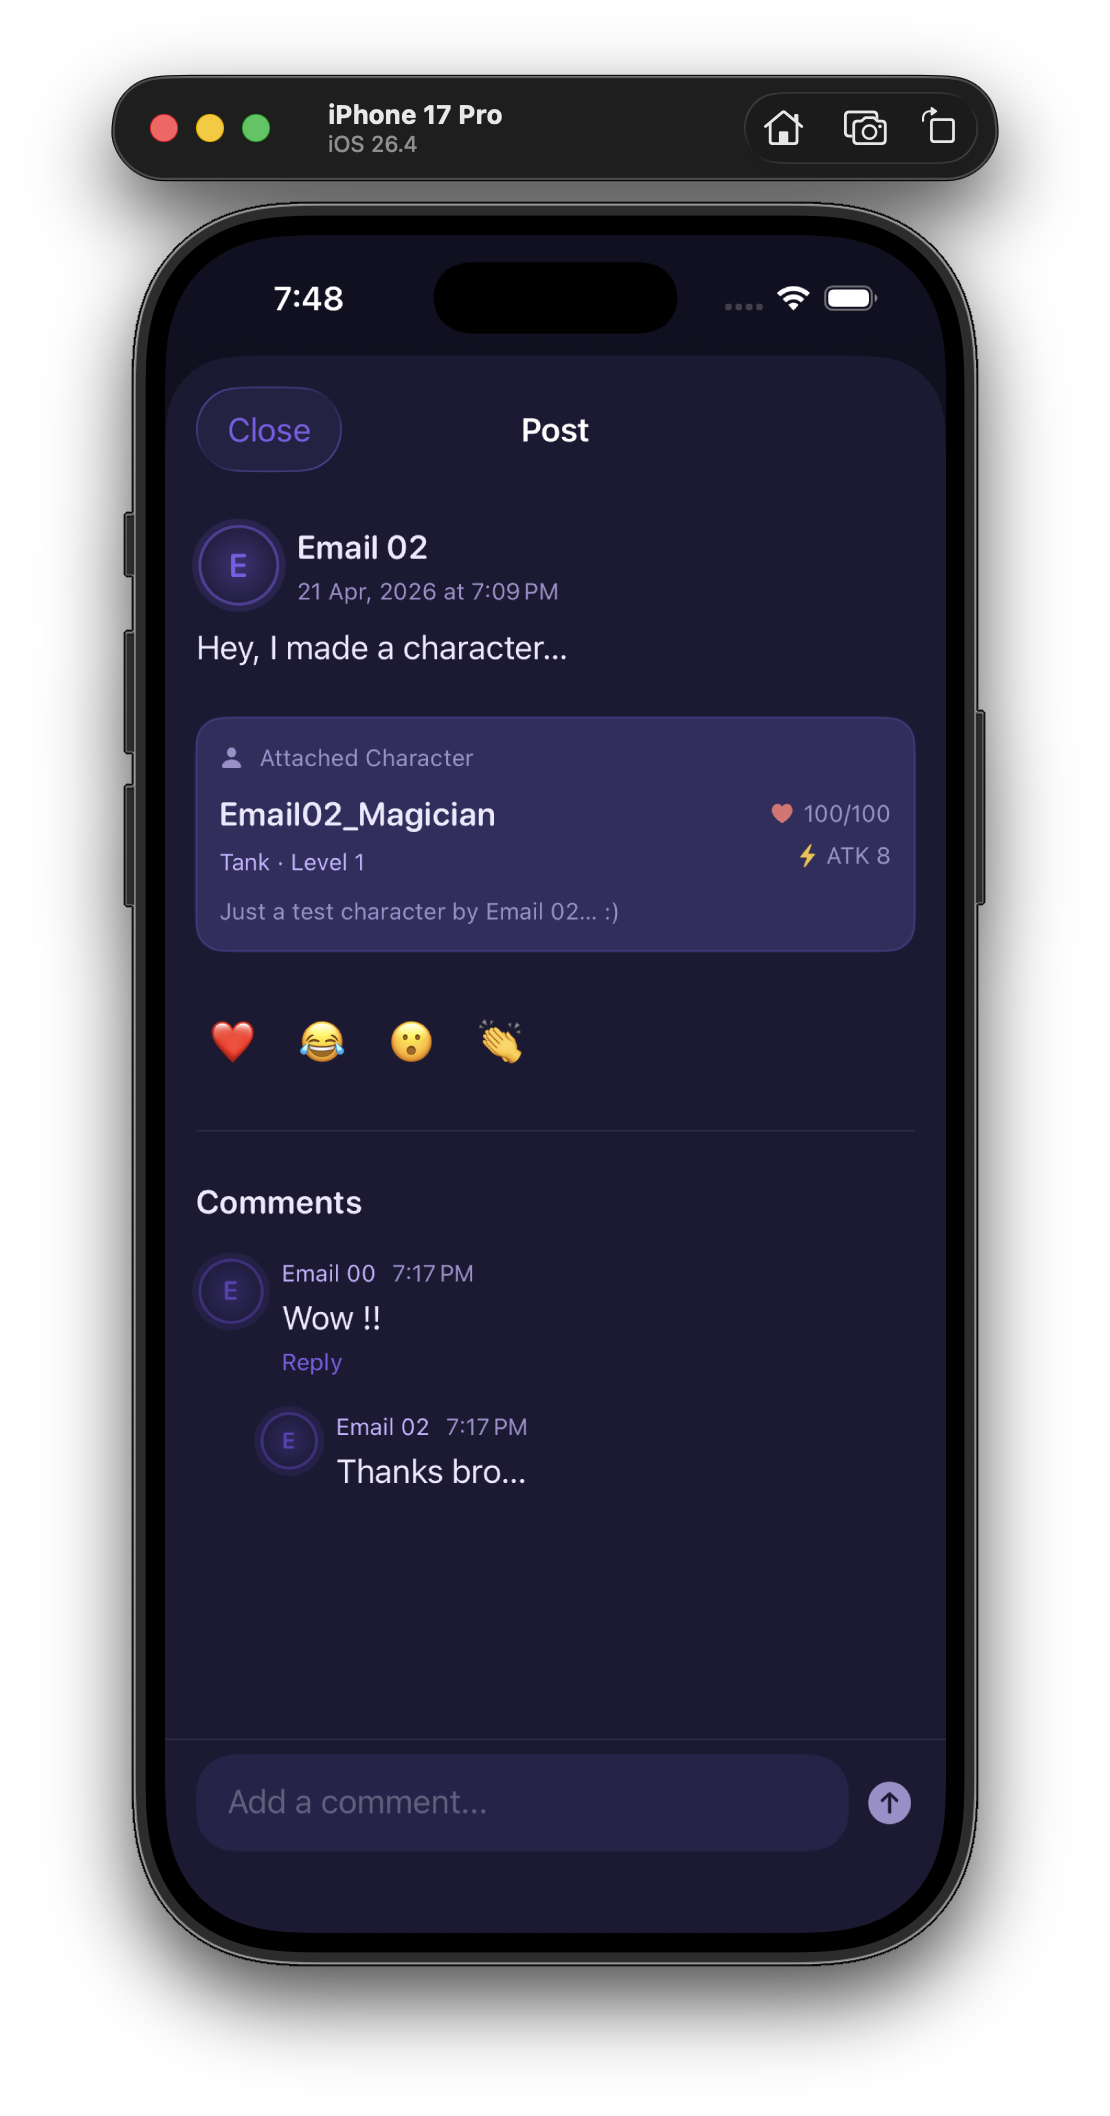
\includegraphics[width=\textwidth]{../images/5_3__post_with_comments_and_replies.png}
    \caption{Comments \& Replies}
  \end{subfigure}
  \caption{Community Feed screens}
\end{figure}

% ─────────────────────────────────────────────────────
\subsection{News Feed}

\begin{itemize}[leftmargin=1.5em]
  \item Dedicated News tab inside the Community screen surfaces live tech and gaming headlines fetched via \texttt{NewsService}.
  \item Article cards display a full-width banner image, source name badge, publication timestamp, headline, and a two-line excerpt with a ``Read full article'' affordance.
\end{itemize}

\begin{figure}[H]
  \centering
  \begin{subfigure}[b]{0.38\textwidth}
    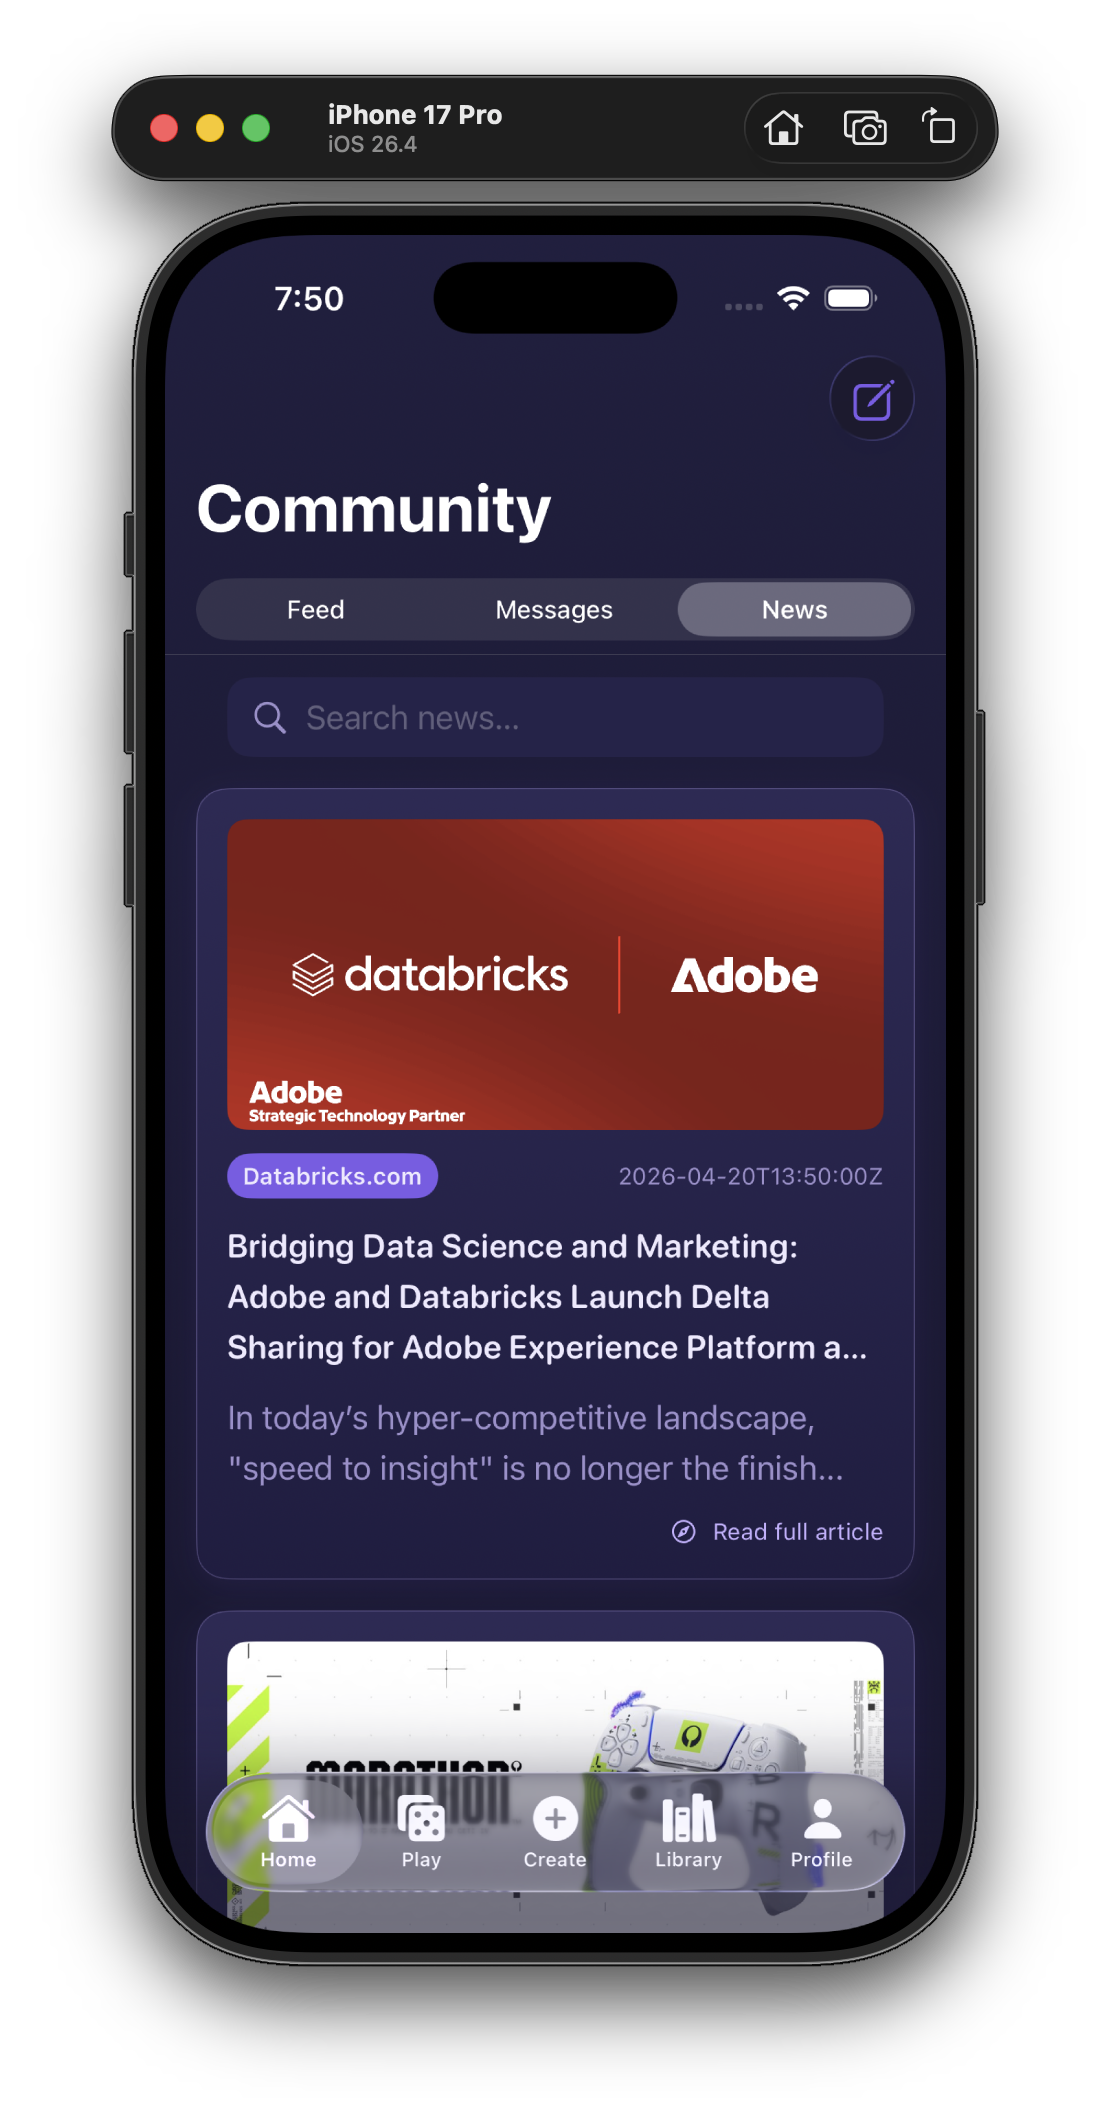
\includegraphics[width=\textwidth]{../images/6_0__news_on_tech_and_gaming.png}
    \caption{News Feed}
  \end{subfigure}
  \caption{Tech \& Gaming News tab}
\end{figure}

% ─────────────────────────────────────────────────────
\subsection{Direct Messaging}

\begin{itemize}[leftmargin=1.5em]
  \item \textbf{People tab} lists all registered users; a ``Message'' button appears only for accepted connections.
  \item Incoming connection requests appear in a card with Accept~($\checkmark$) and Decline~($\times$) buttons.
  \item One-on-one conversation screen: sender bubbles are purple (right), receiver bubbles are dark (left), each with a timestamp below.
  \item Conversation list (Messages tab) shows latest message preview, peer name, and elapsed time badge; updates in real time via Firestore listener.
\end{itemize}

\begin{figure}[H]
  \centering
  \begin{subfigure}[b]{0.3\textwidth}
    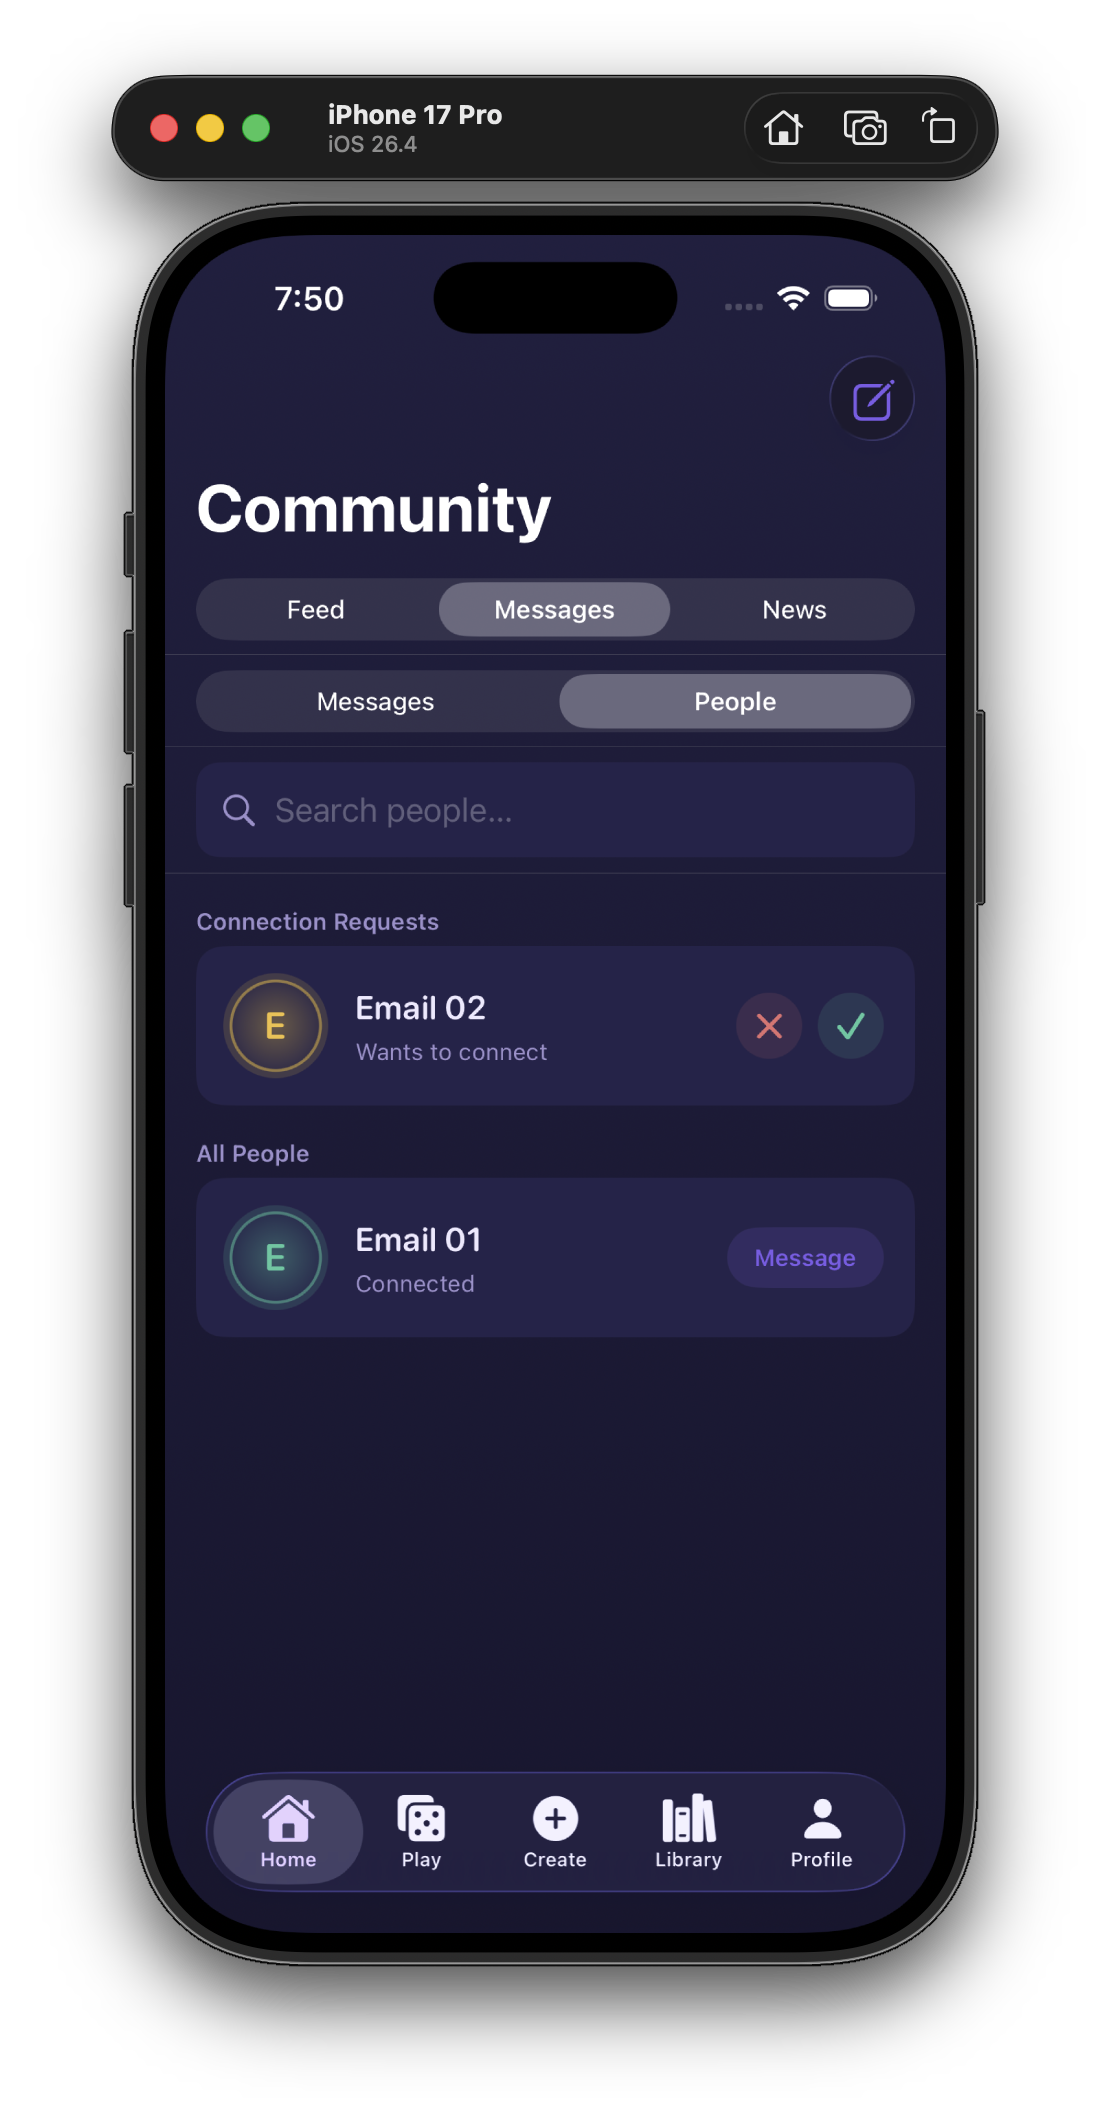
\includegraphics[width=\textwidth]{../images/7_0__message_request_approve_decline.png}
    \caption{Connection Request}
  \end{subfigure}
  \hfill
  \begin{subfigure}[b]{0.3\textwidth}
    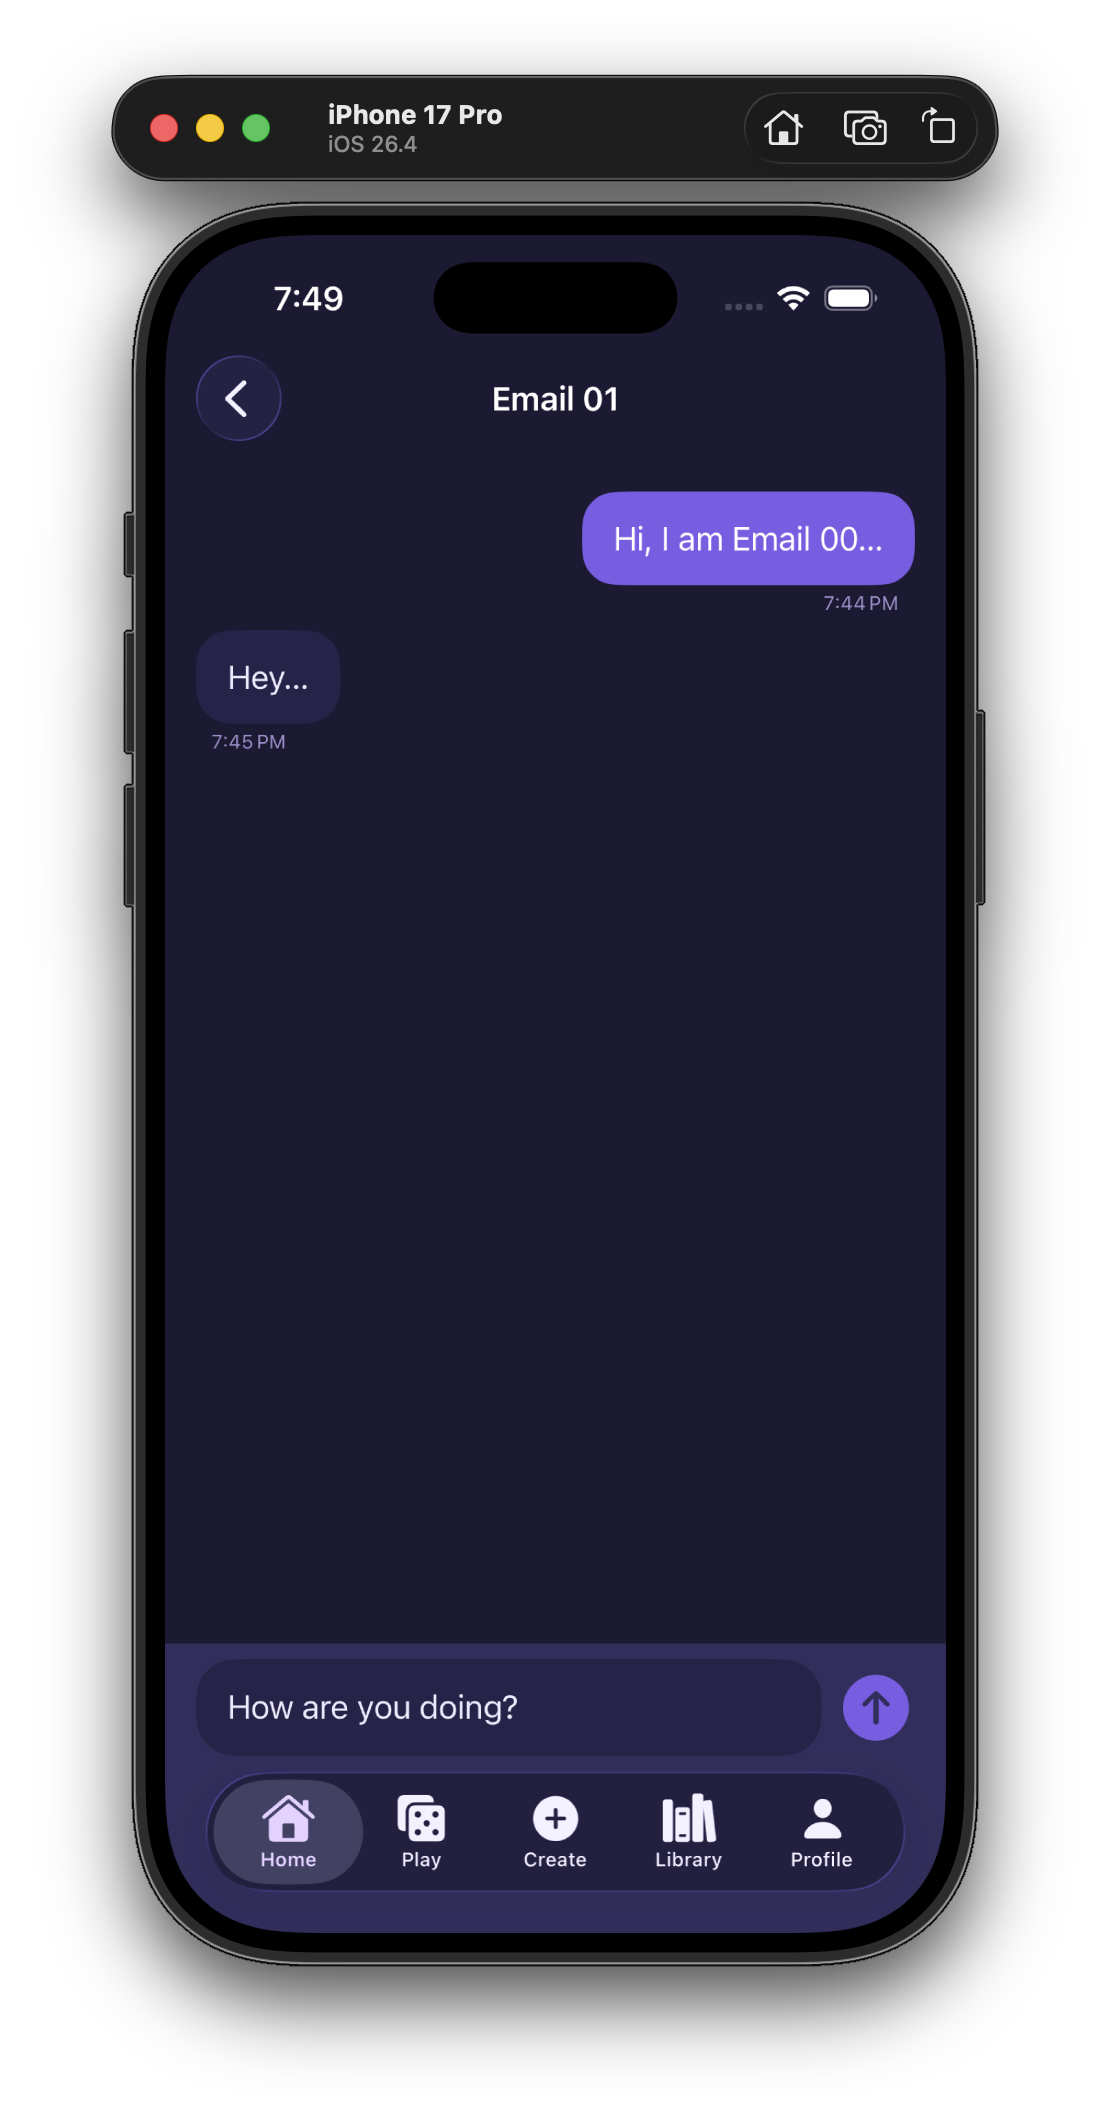
\includegraphics[width=\textwidth]{../images/7_3__message_writing.png}
    \caption{Chat Window}
  \end{subfigure}
  \hfill
  \begin{subfigure}[b]{0.3\textwidth}
    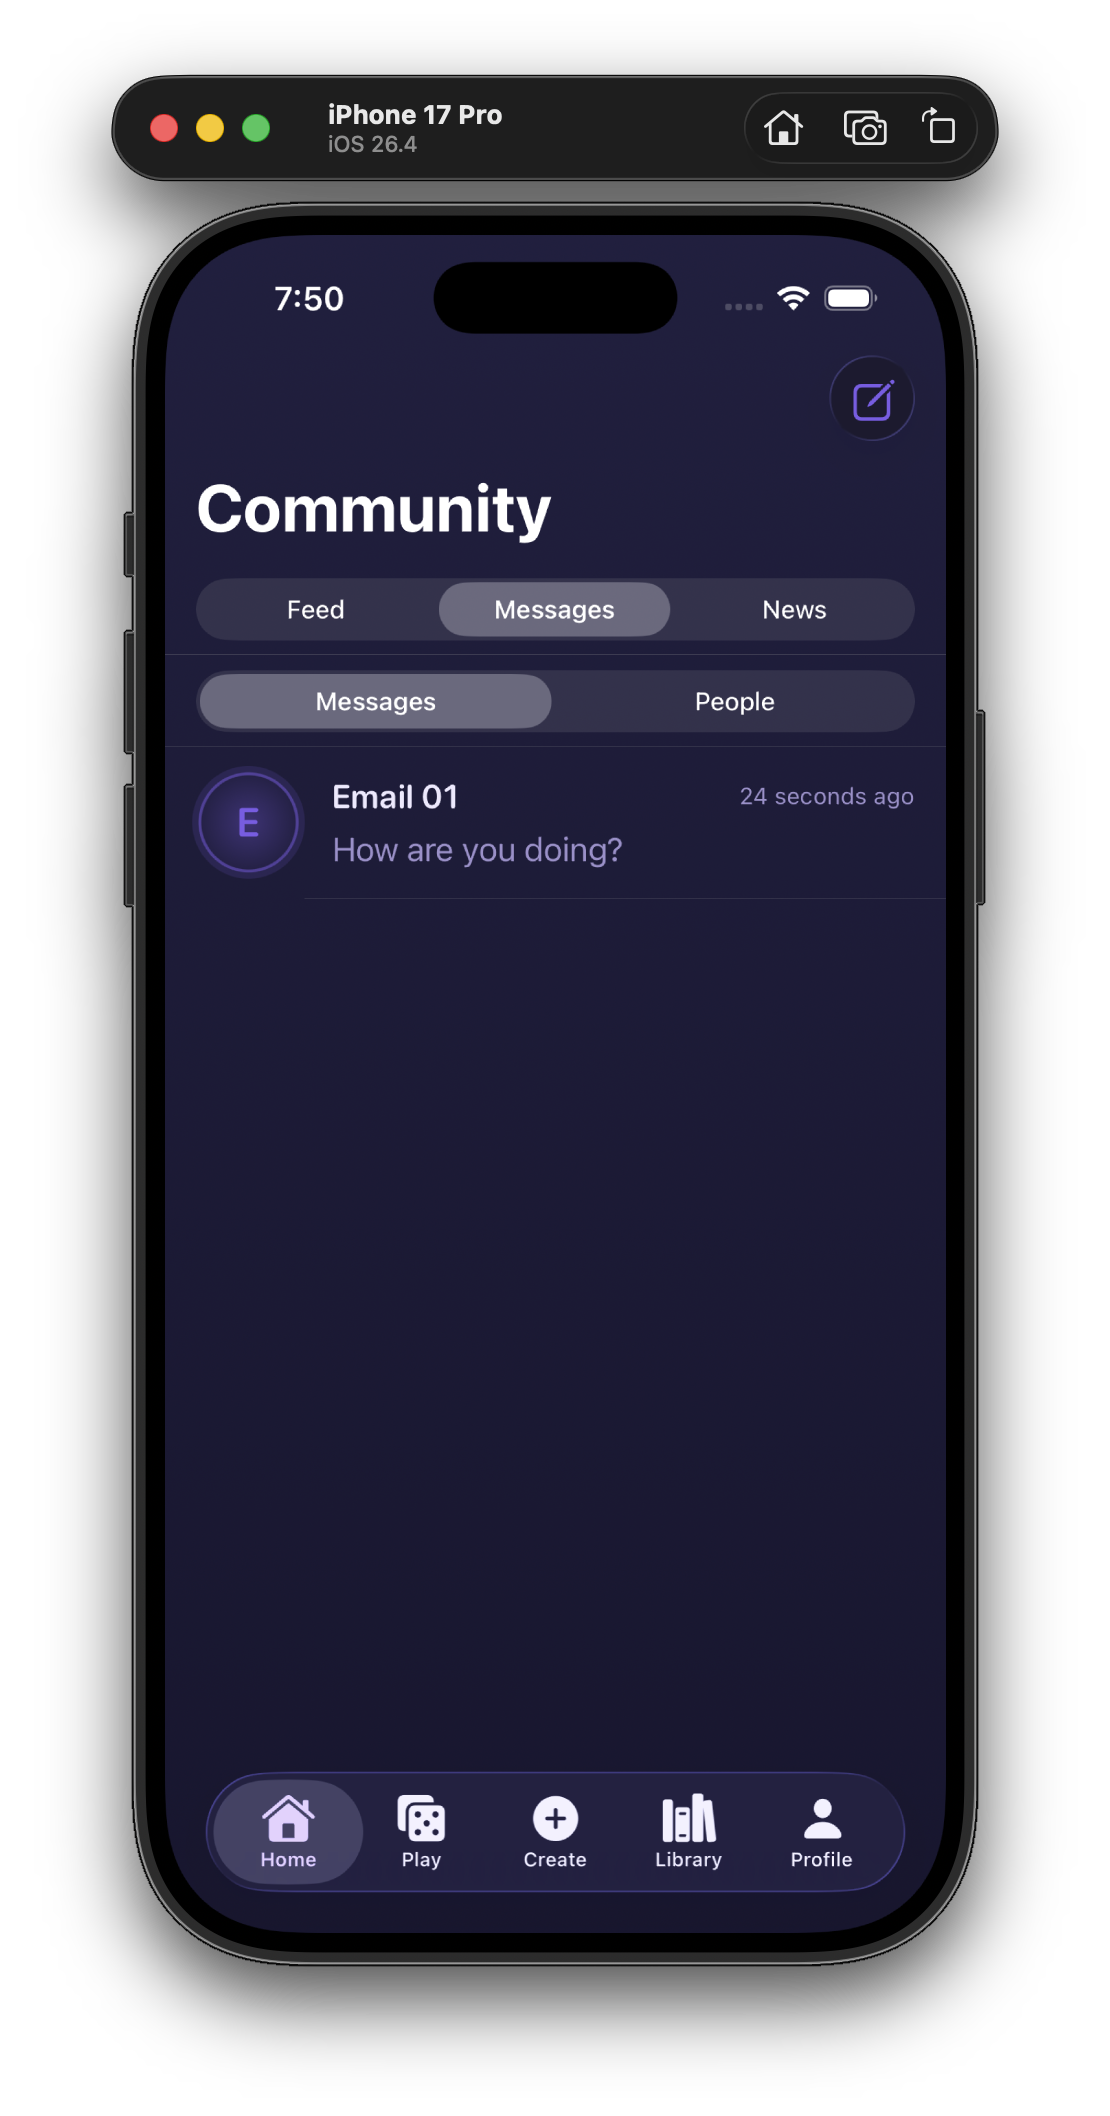
\includegraphics[width=\textwidth]{../images/7_5__message_inbox_list.png}
    \caption{Conversation List}
  \end{subfigure}
  \caption{Direct Messaging screens}
\end{figure}

% ─────────────────────────────────────────────────────
\subsection{Game — Party Assembly}

\begin{itemize}[leftmargin=1.5em]
  \item Three tabs in the Play screen: \textbf{Campaign} (built-in five-act story), \textbf{Community} (user-published stories), \textbf{Sessions} (multiplayer lobbies).
  \item Party assembly screen: bot companion count slider (1--5), character browser in list or grid layout, tap a card to toggle BOT / HERO designation (star badge for hero).
  \item ``Begin Adventure'' button activates once a hero is selected; bot companions fill remaining slots.
  \item A \textbf{Multiplayer} button opens a session lobby where players are invited by UID and assigned characters.
\end{itemize}

\begin{figure}[H]
  \centering
  \begin{subfigure}[b]{0.3\textwidth}
    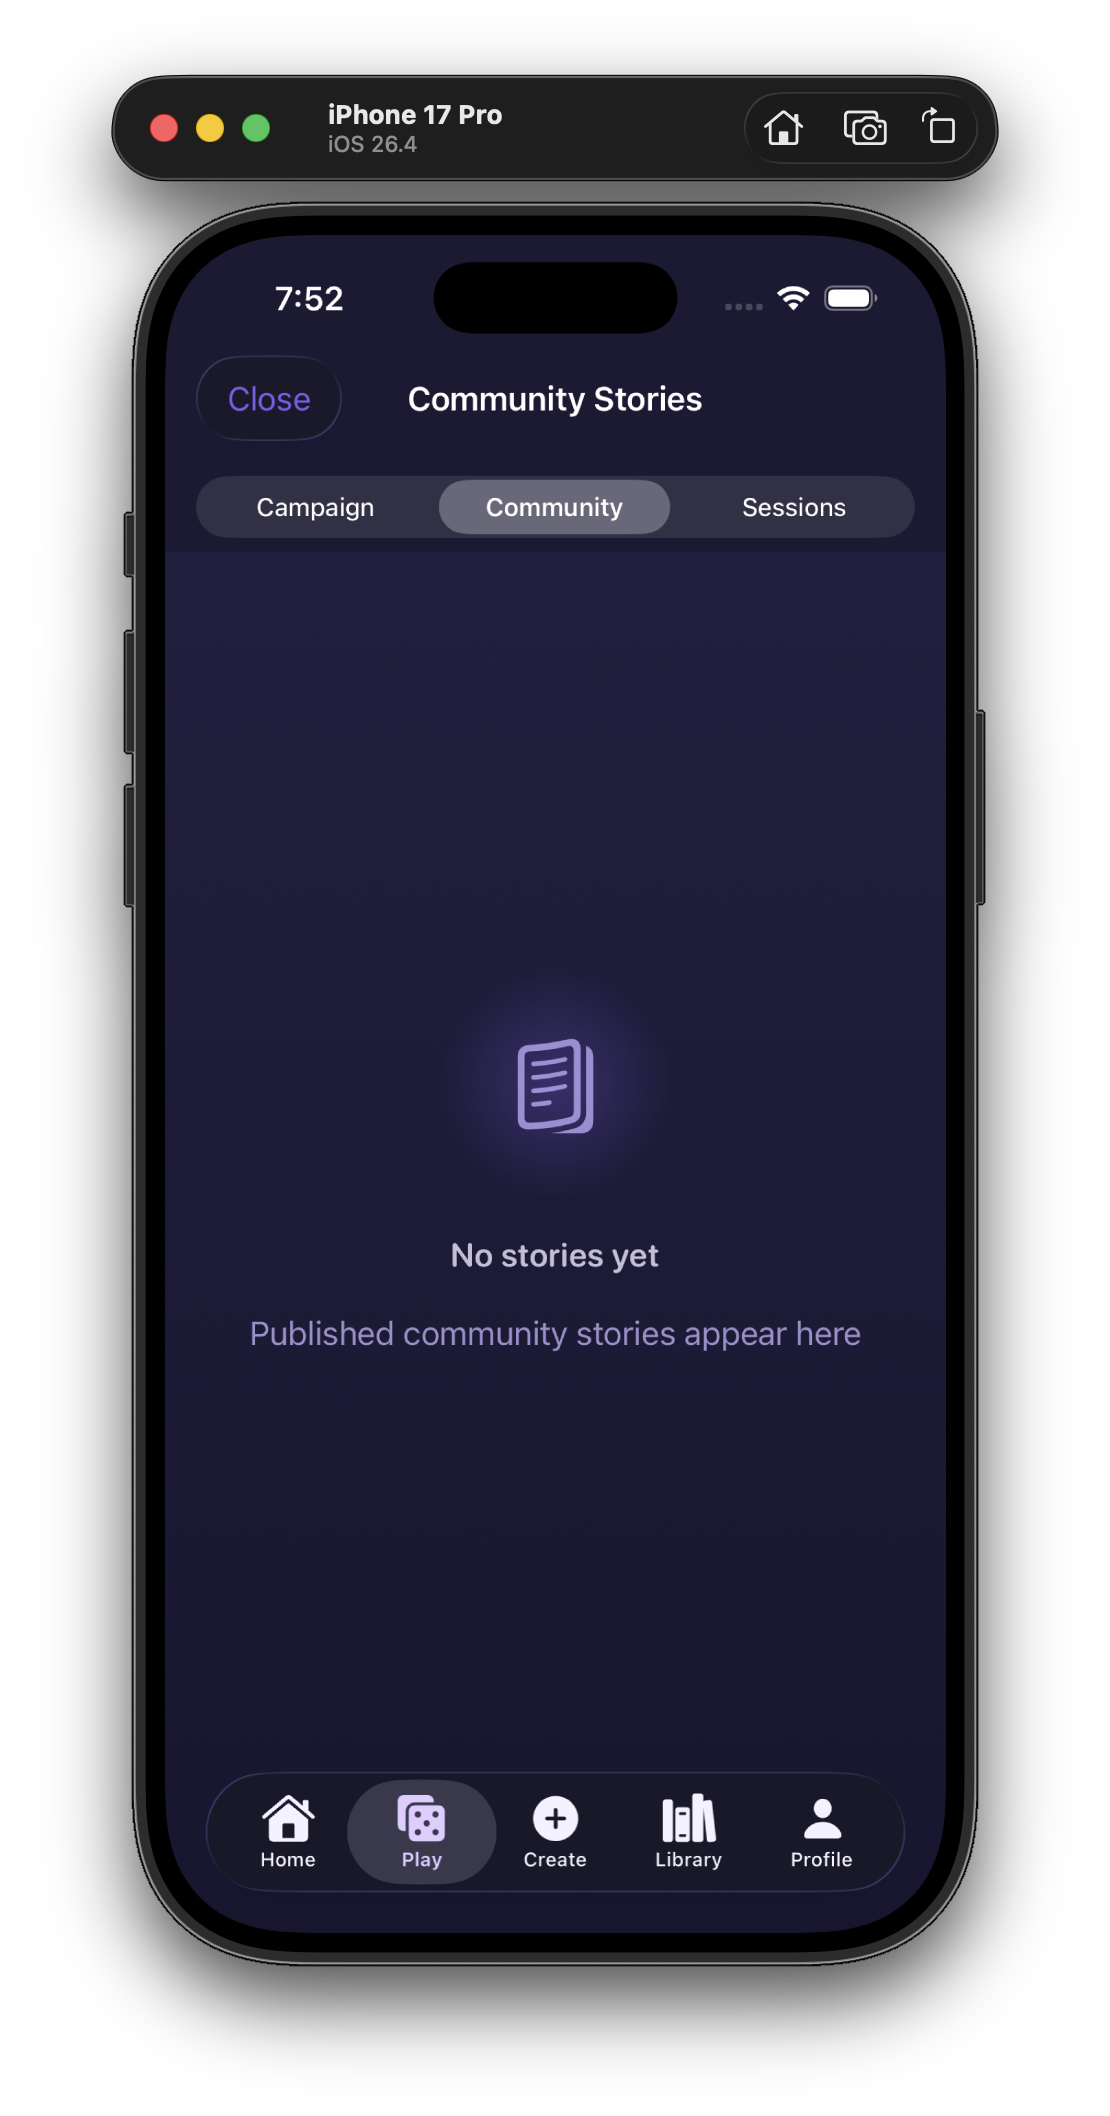
\includegraphics[width=\textwidth]{../images/8_0__play_community.png}
    \caption{Community Stories}
  \end{subfigure}
  \hfill
  \begin{subfigure}[b]{0.3\textwidth}
    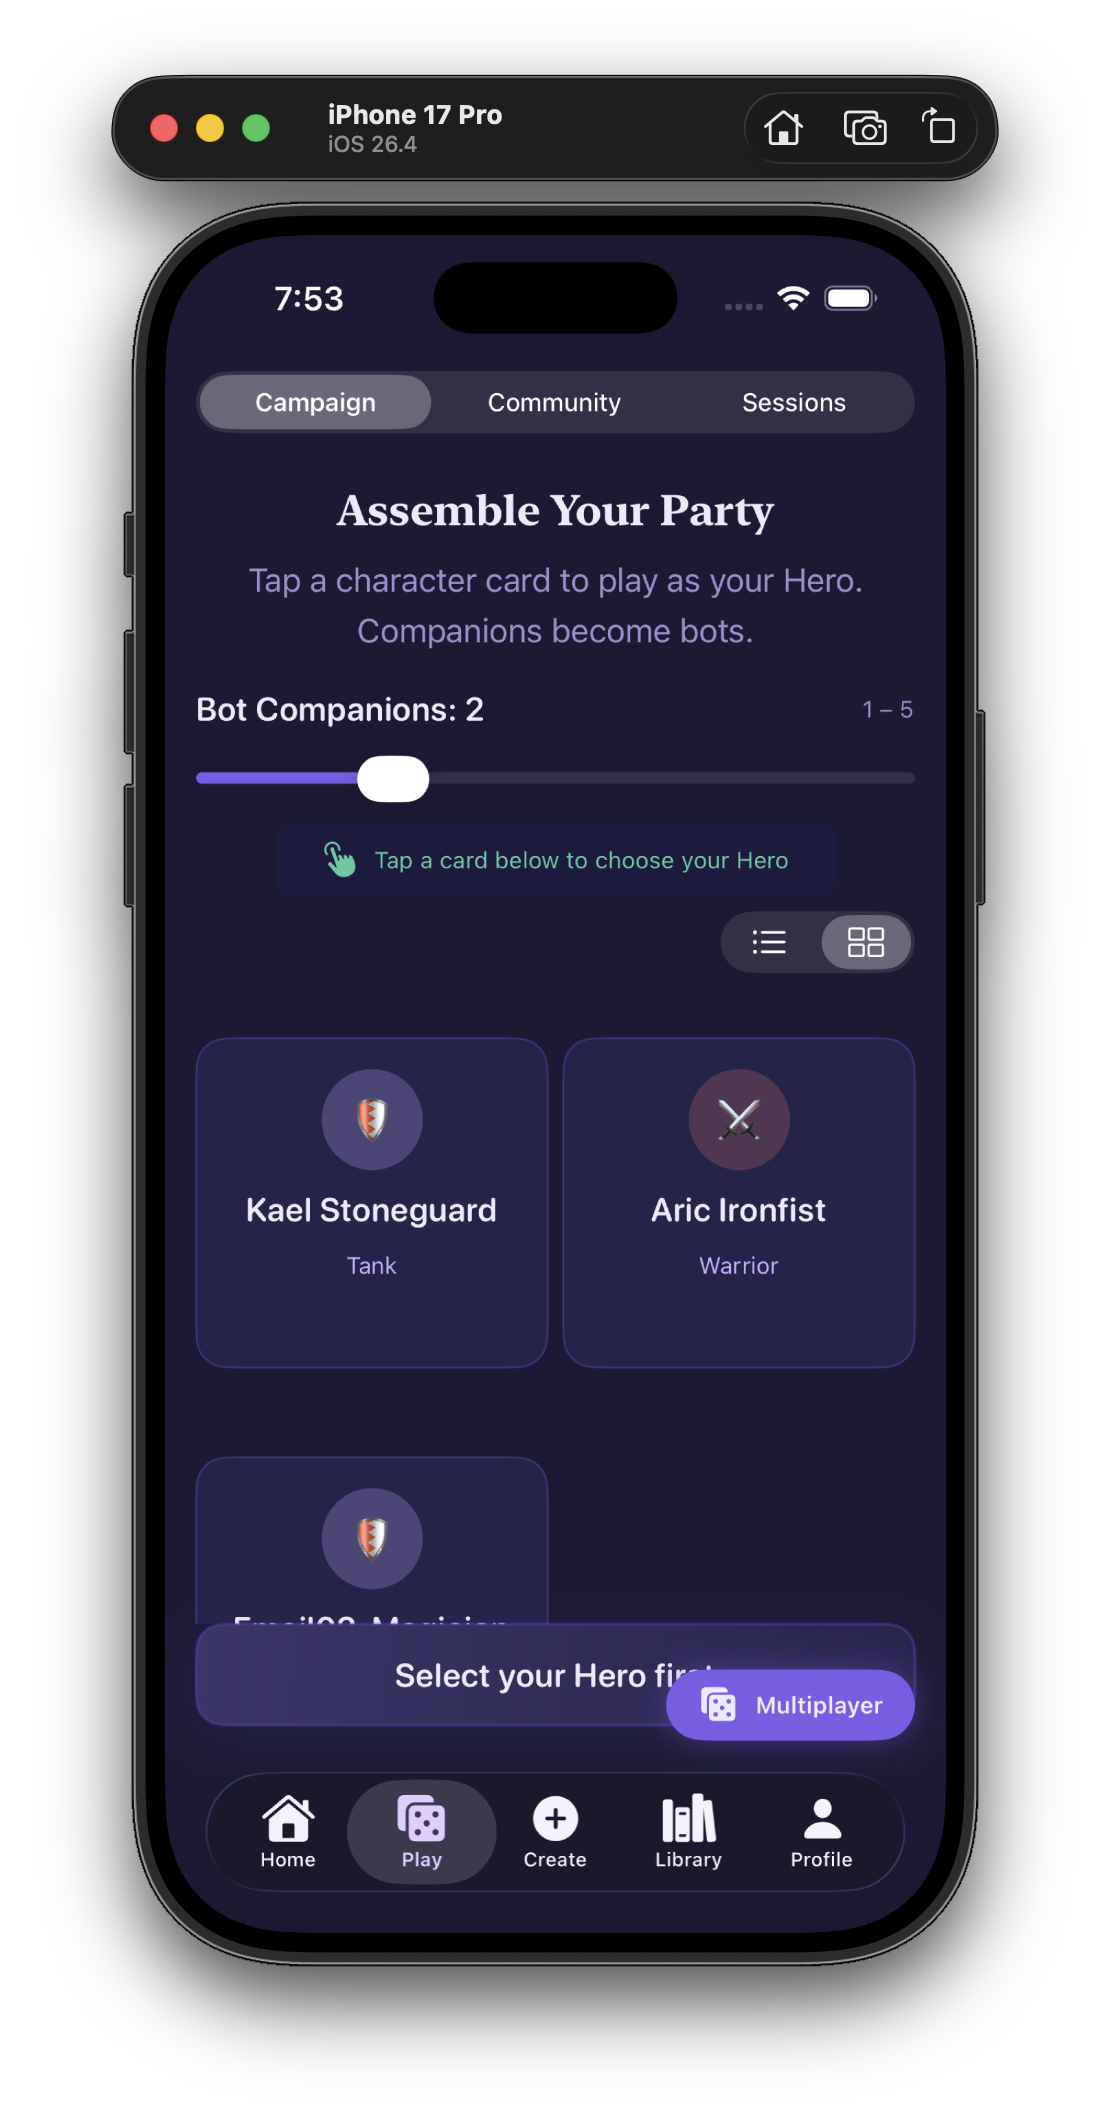
\includegraphics[width=\textwidth]{../images/8_2__play_start_characters_grid.png}
    \caption{Character Grid}
  \end{subfigure}
  \hfill
  \begin{subfigure}[b]{0.3\textwidth}
    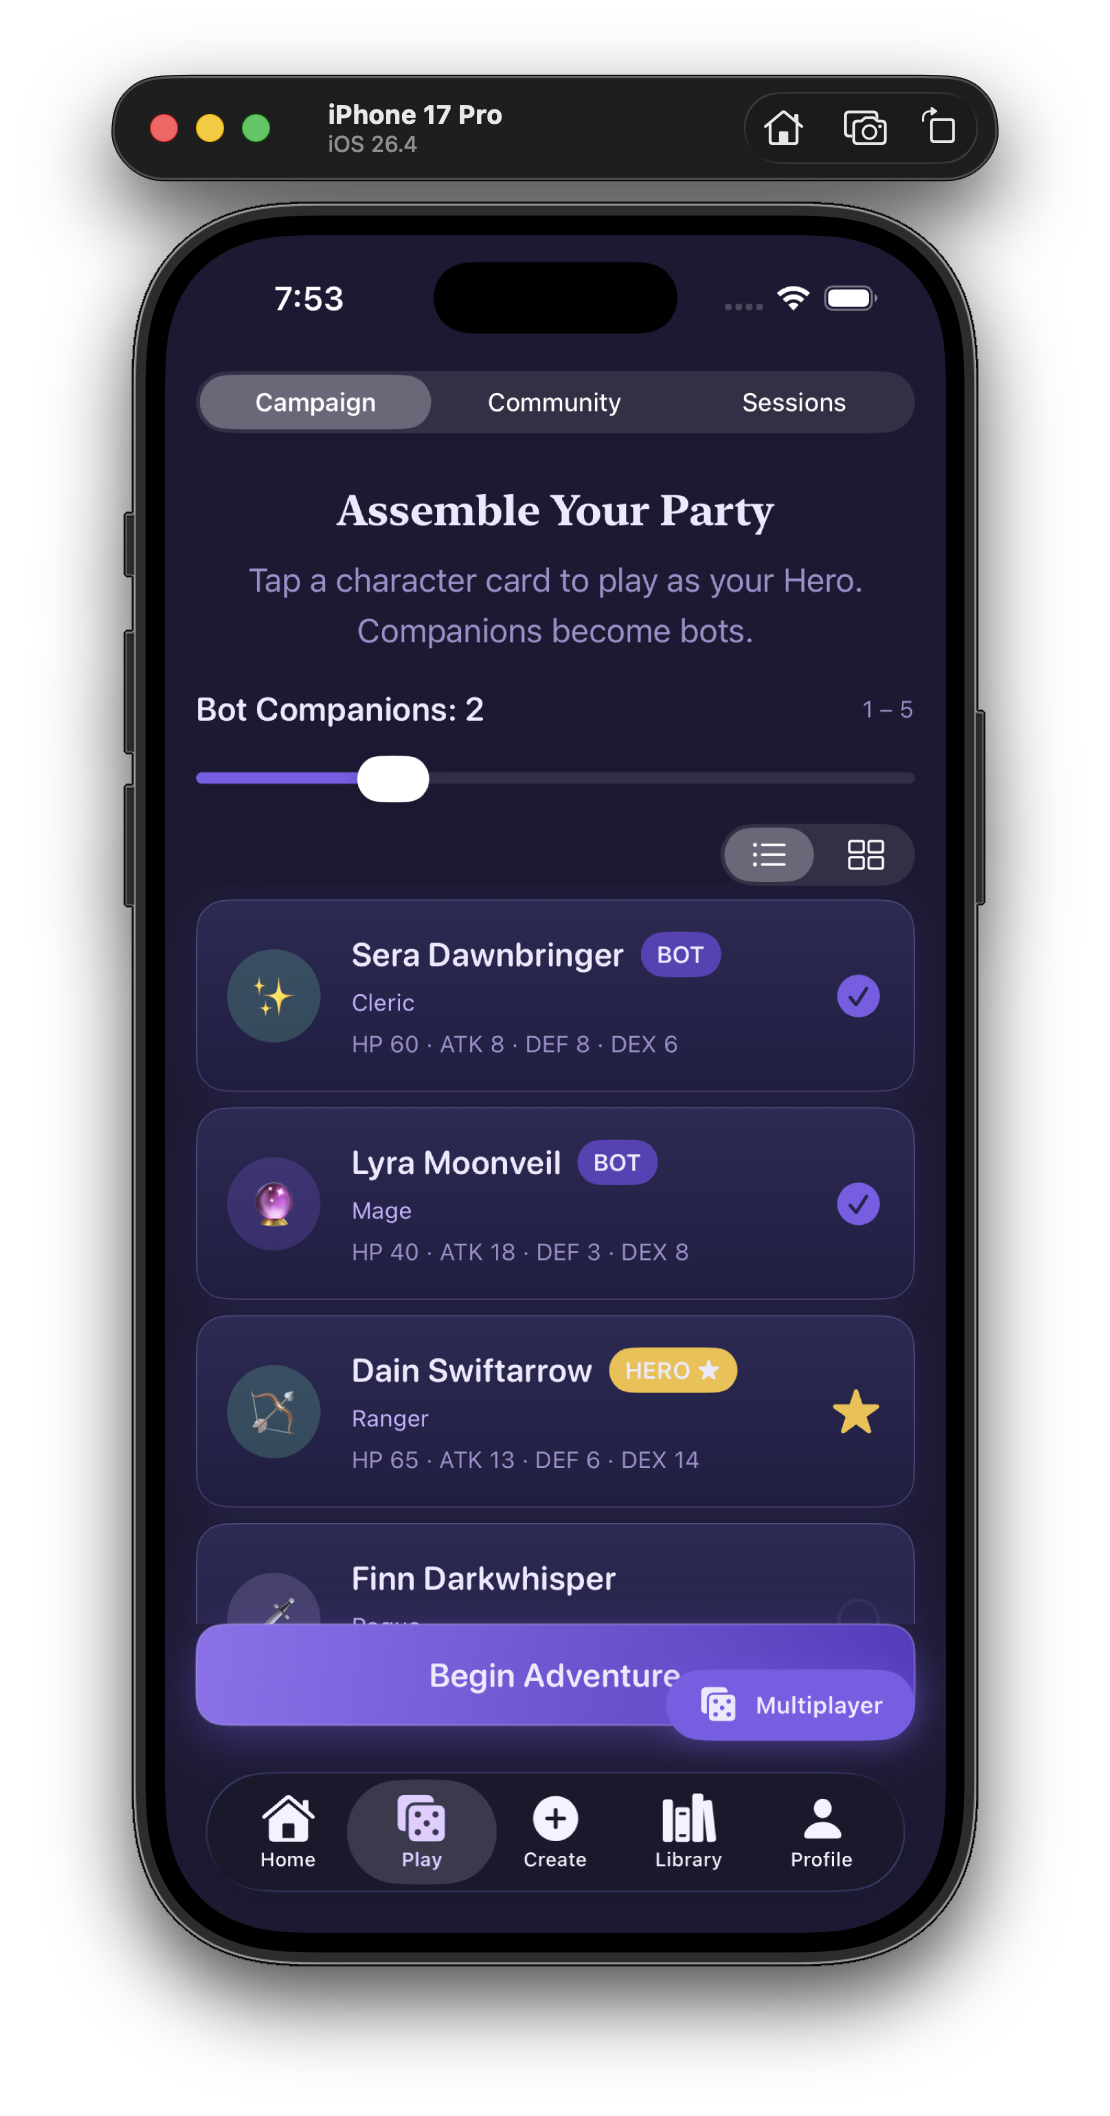
\includegraphics[width=\textwidth]{../images/8_3__play_select_your_hero.png}
    \caption{Select Hero}
  \end{subfigure}
  \caption{Game — Party Assembly screens}
\end{figure}

% ─────────────────────────────────────────────────────
\subsection{Game — Scene Engine}

Four scene types drive the narrative:

\textbf{Exploration} — Act title shown in a styled header. Gemini-narrated text panel fills the centre. Up to four branching choice buttons sit below. Party member health bars are pinned to the bottom with archetype icon, name abbreviation, and a colour-coded HP bar.

\textbf{Combat} — Two-row battlefield: emoji-avatar enemies (with name labels and red HP bars) in the top row; party members (with archetype icons and green/amber HP bars) in the bottom row. Player-turn action panel shows Attack, Defend, and Skill buttons. On bot and enemy turns, each action resolves live and appends a line to the combat log (e.g.\ ``Sera Dawnbringer attacks Goblin Scout for 6'', ``criticalFail'').

\textbf{Skill Check} — Narrative context card shown at top. A stat badge (e.g.\ DEX) and DC number indicate the challenge. A large ``Roll d20'' button triggers a \texttt{rotation3DEffect}-powered dice animation; the resolved number appears with a green or red colour depending on pass/fail.

\begin{figure}[H]
  \centering
  \begin{subfigure}[b]{0.3\textwidth}
    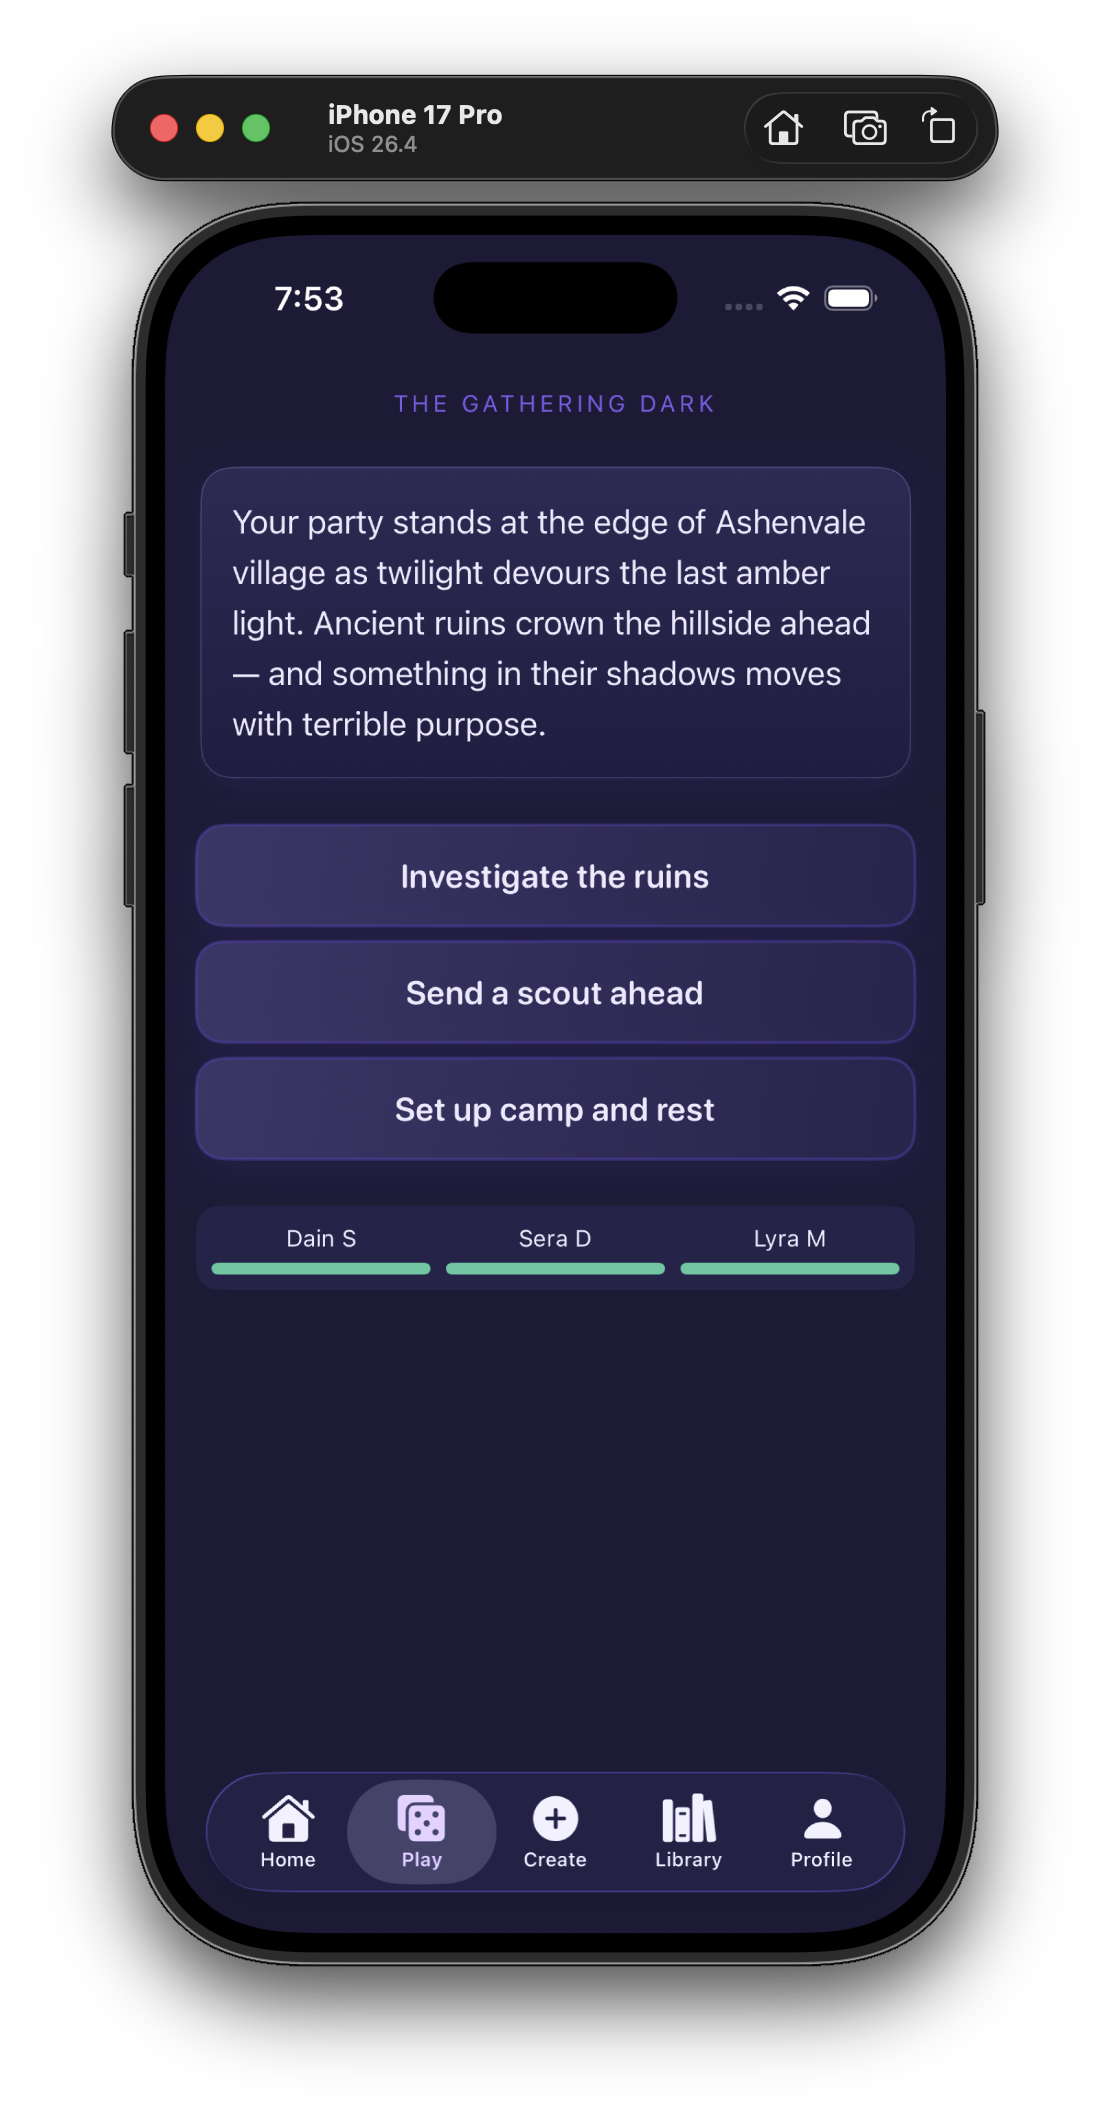
\includegraphics[width=\textwidth]{../images/9_0__play_ground_0.png}
    \caption{Exploration}
  \end{subfigure}
  \hfill
  \begin{subfigure}[b]{0.3\textwidth}
    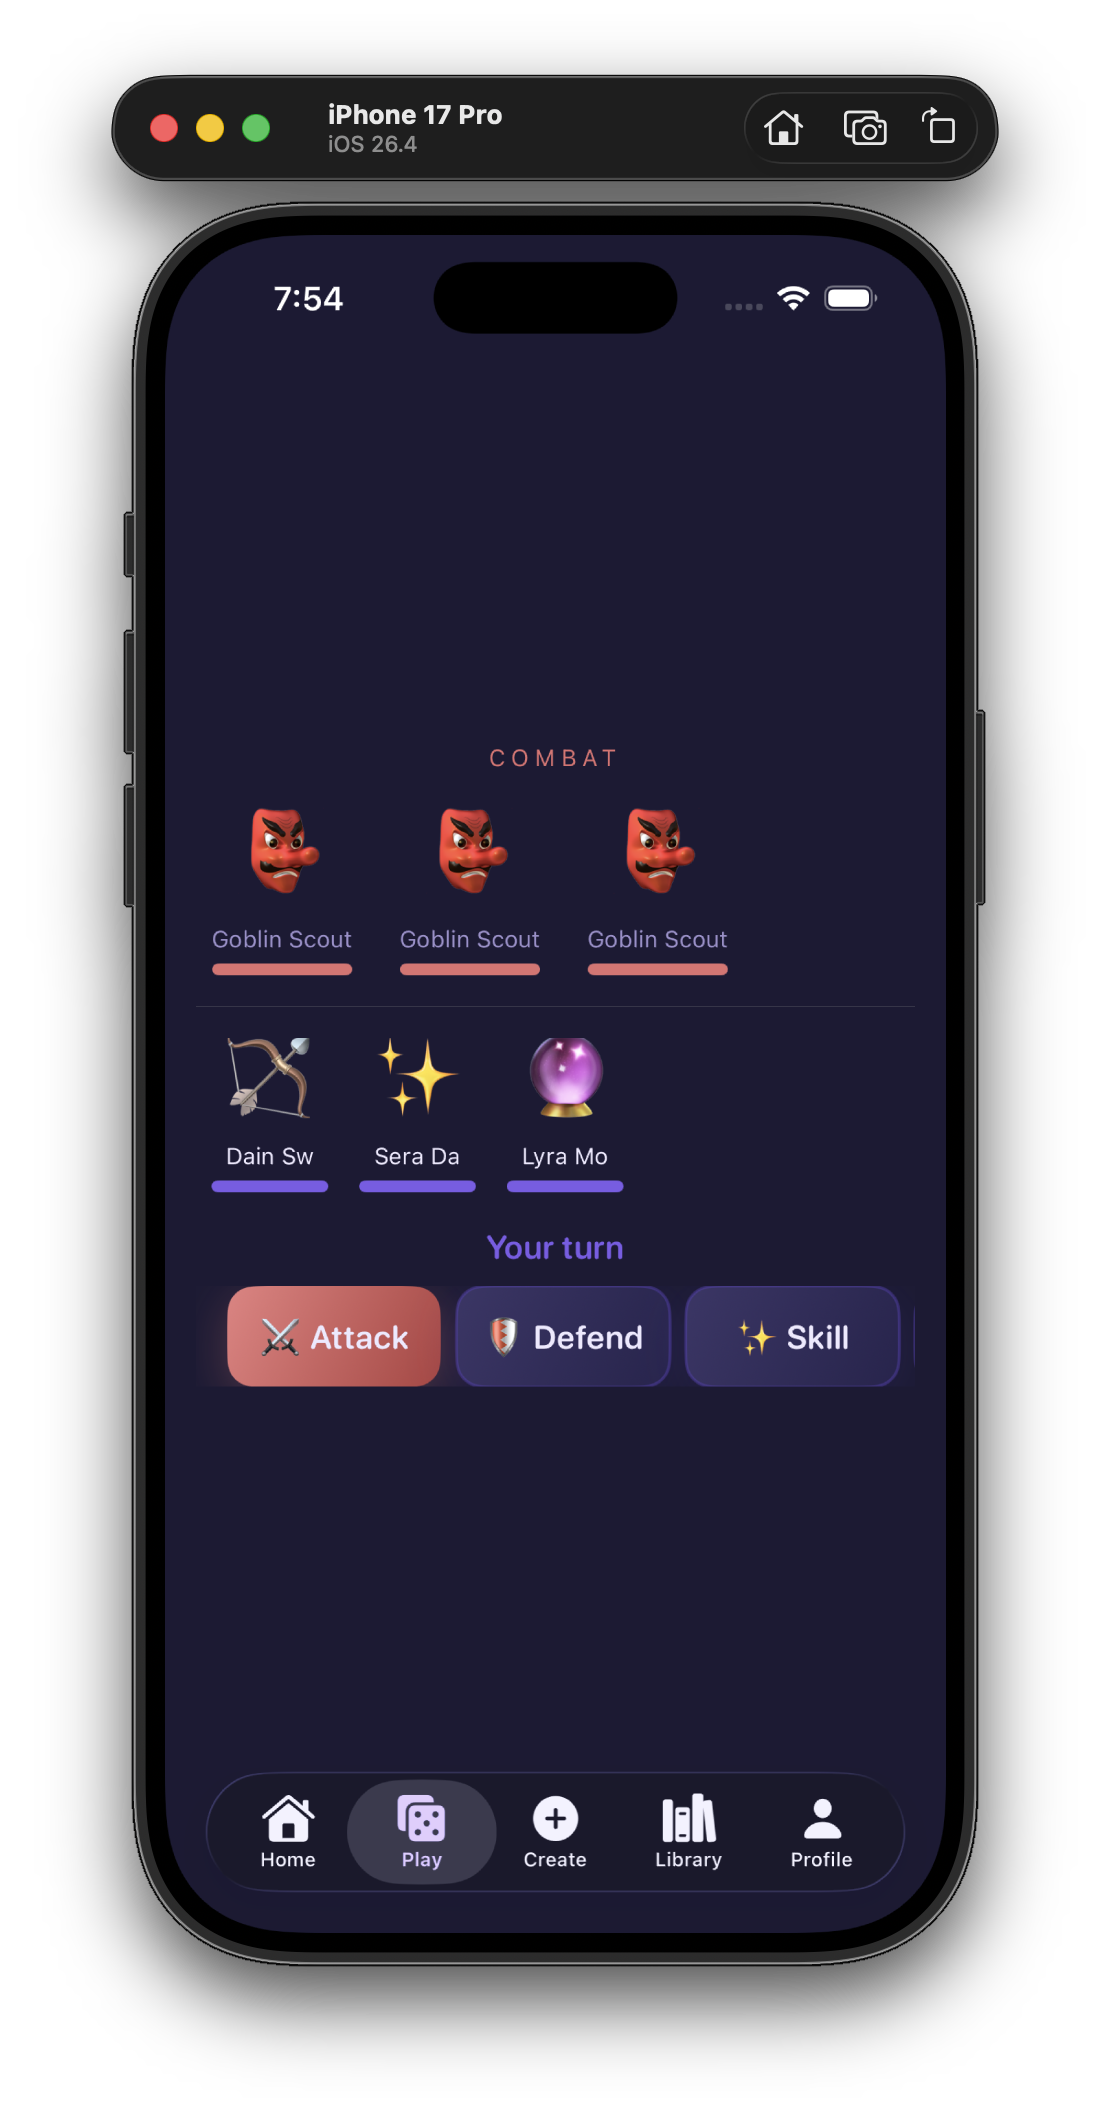
\includegraphics[width=\textwidth]{../images/9_2__play_combat.png}
    \caption{Combat — Player Turn}
  \end{subfigure}
  \hfill
  \begin{subfigure}[b]{0.3\textwidth}
    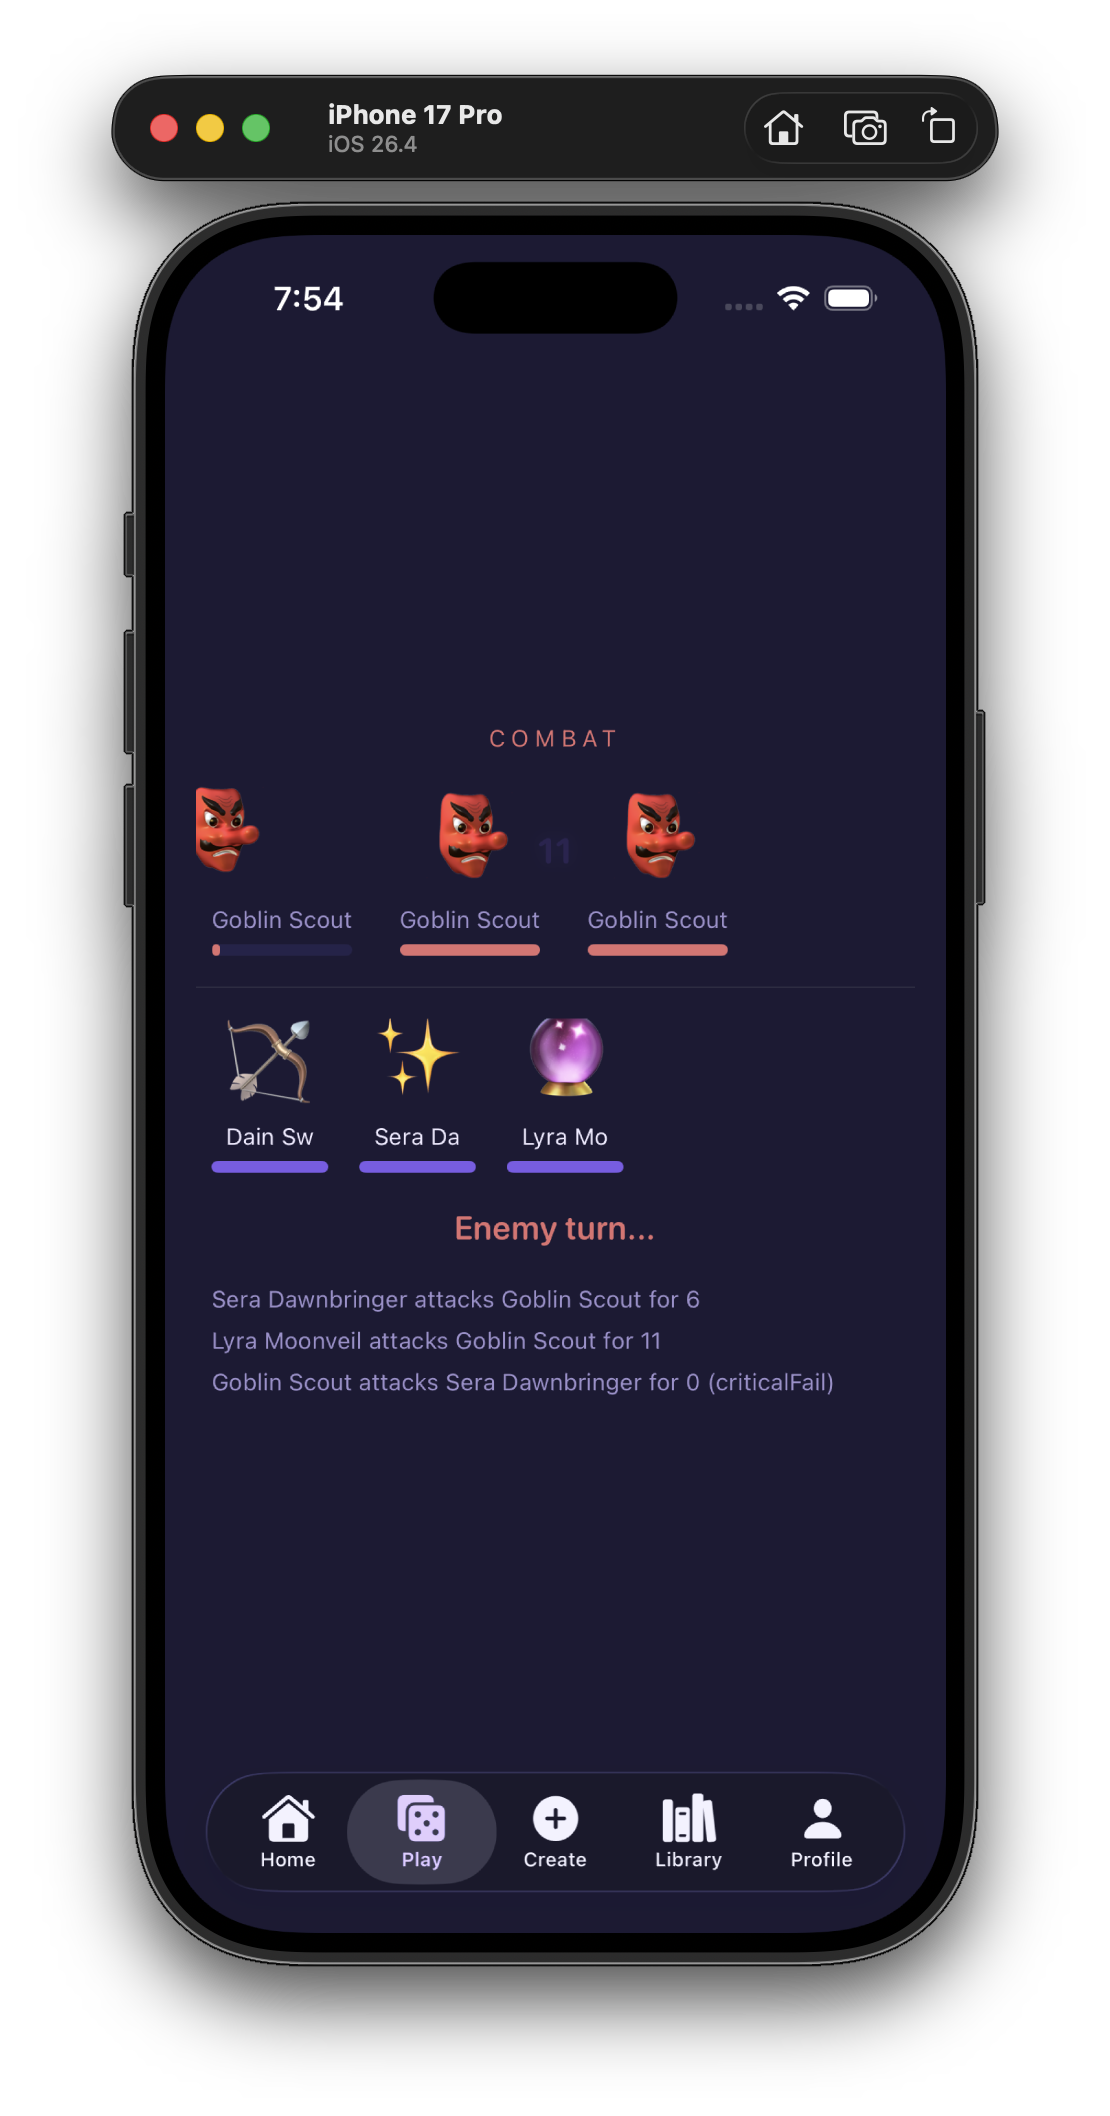
\includegraphics[width=\textwidth]{../images/9_3__play_bot_enemy.png}
    \caption{Combat — Enemy Turn}
  \end{subfigure}
  \caption{Game Scene Engine — Exploration and Combat}
\end{figure}

\begin{figure}[H]
  \centering
  \begin{subfigure}[b]{0.3\textwidth}
    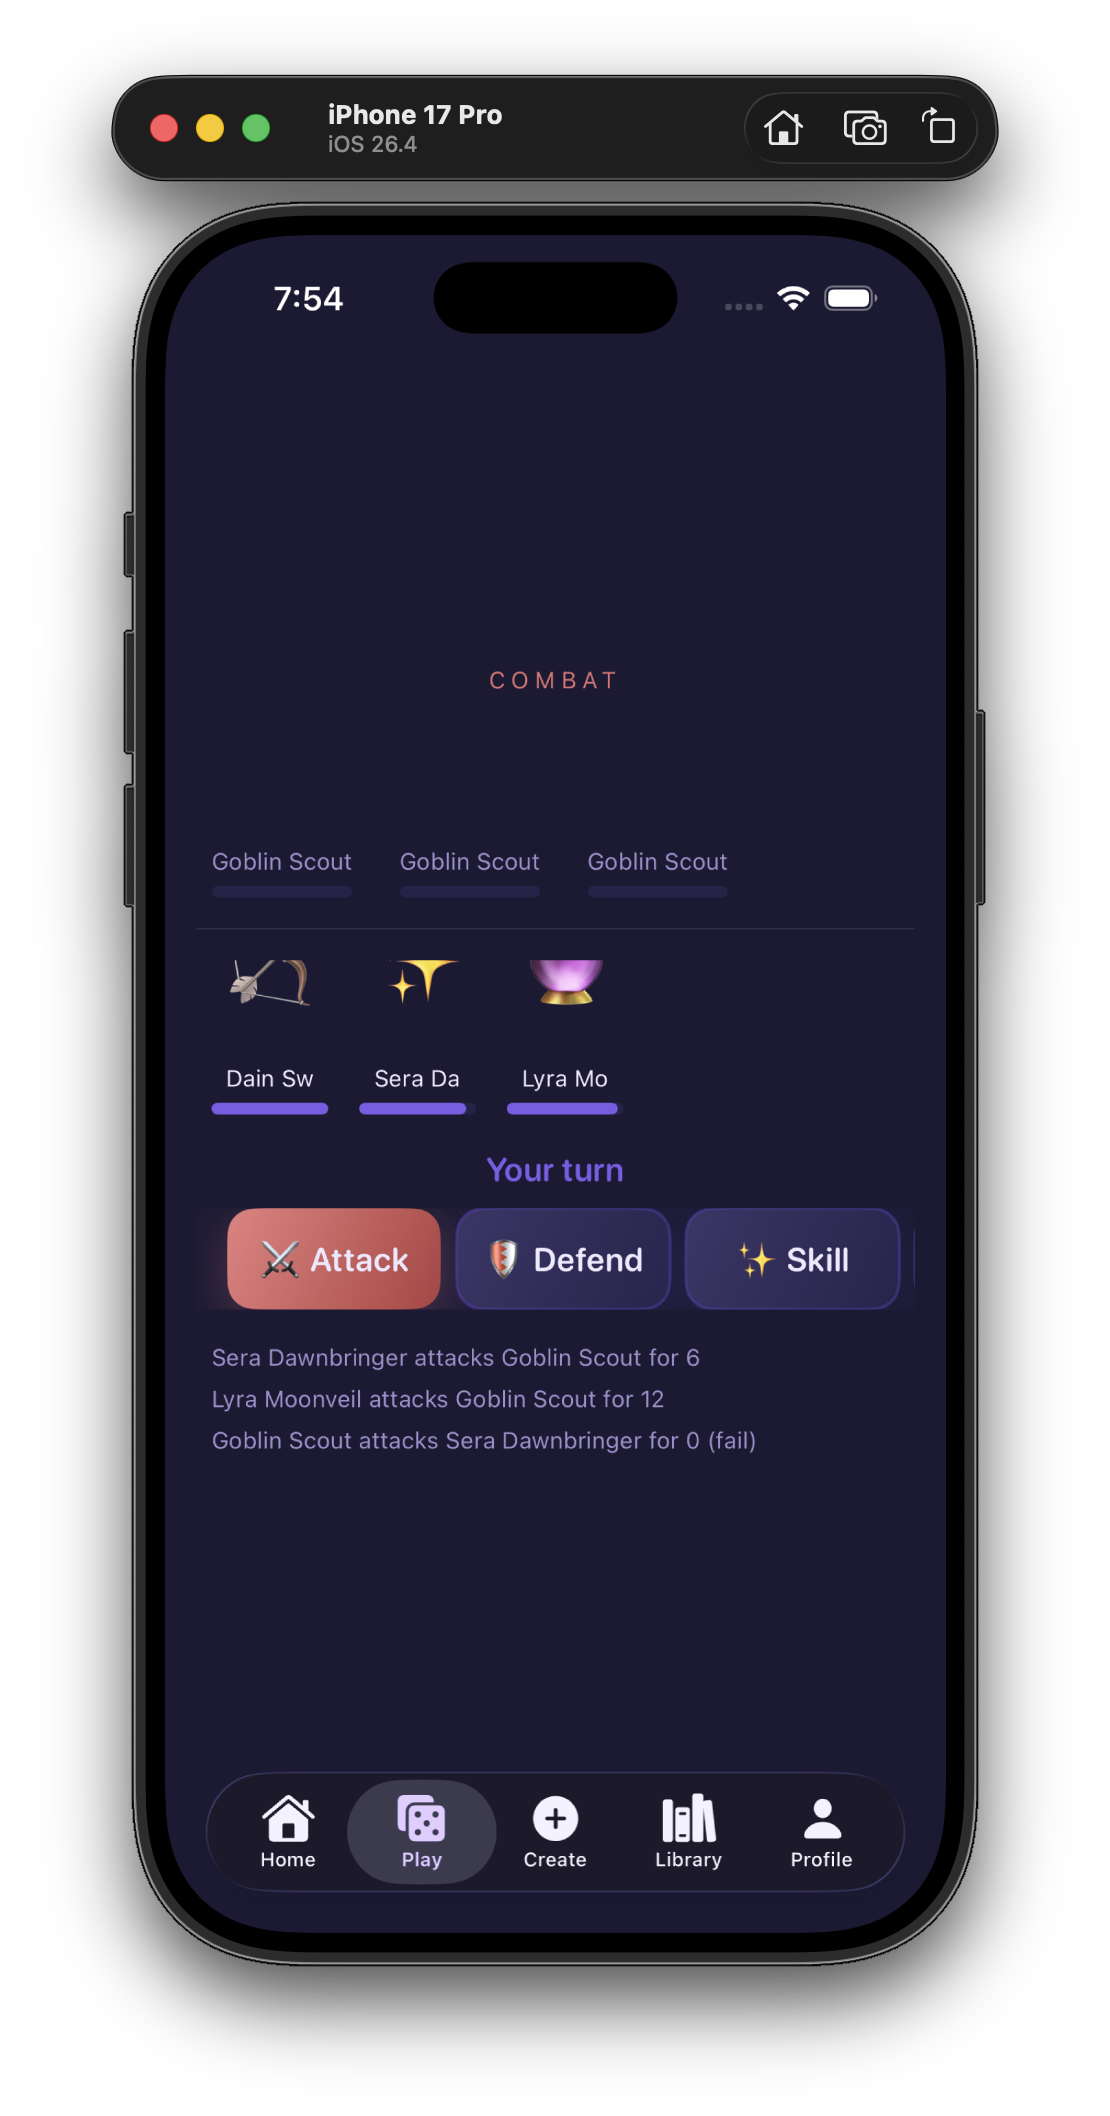
\includegraphics[width=\textwidth]{../images/9_5__play_combat_contunue_0.png}
    \caption{Combat Continued}
  \end{subfigure}
  \hfill
  \begin{subfigure}[b]{0.3\textwidth}
    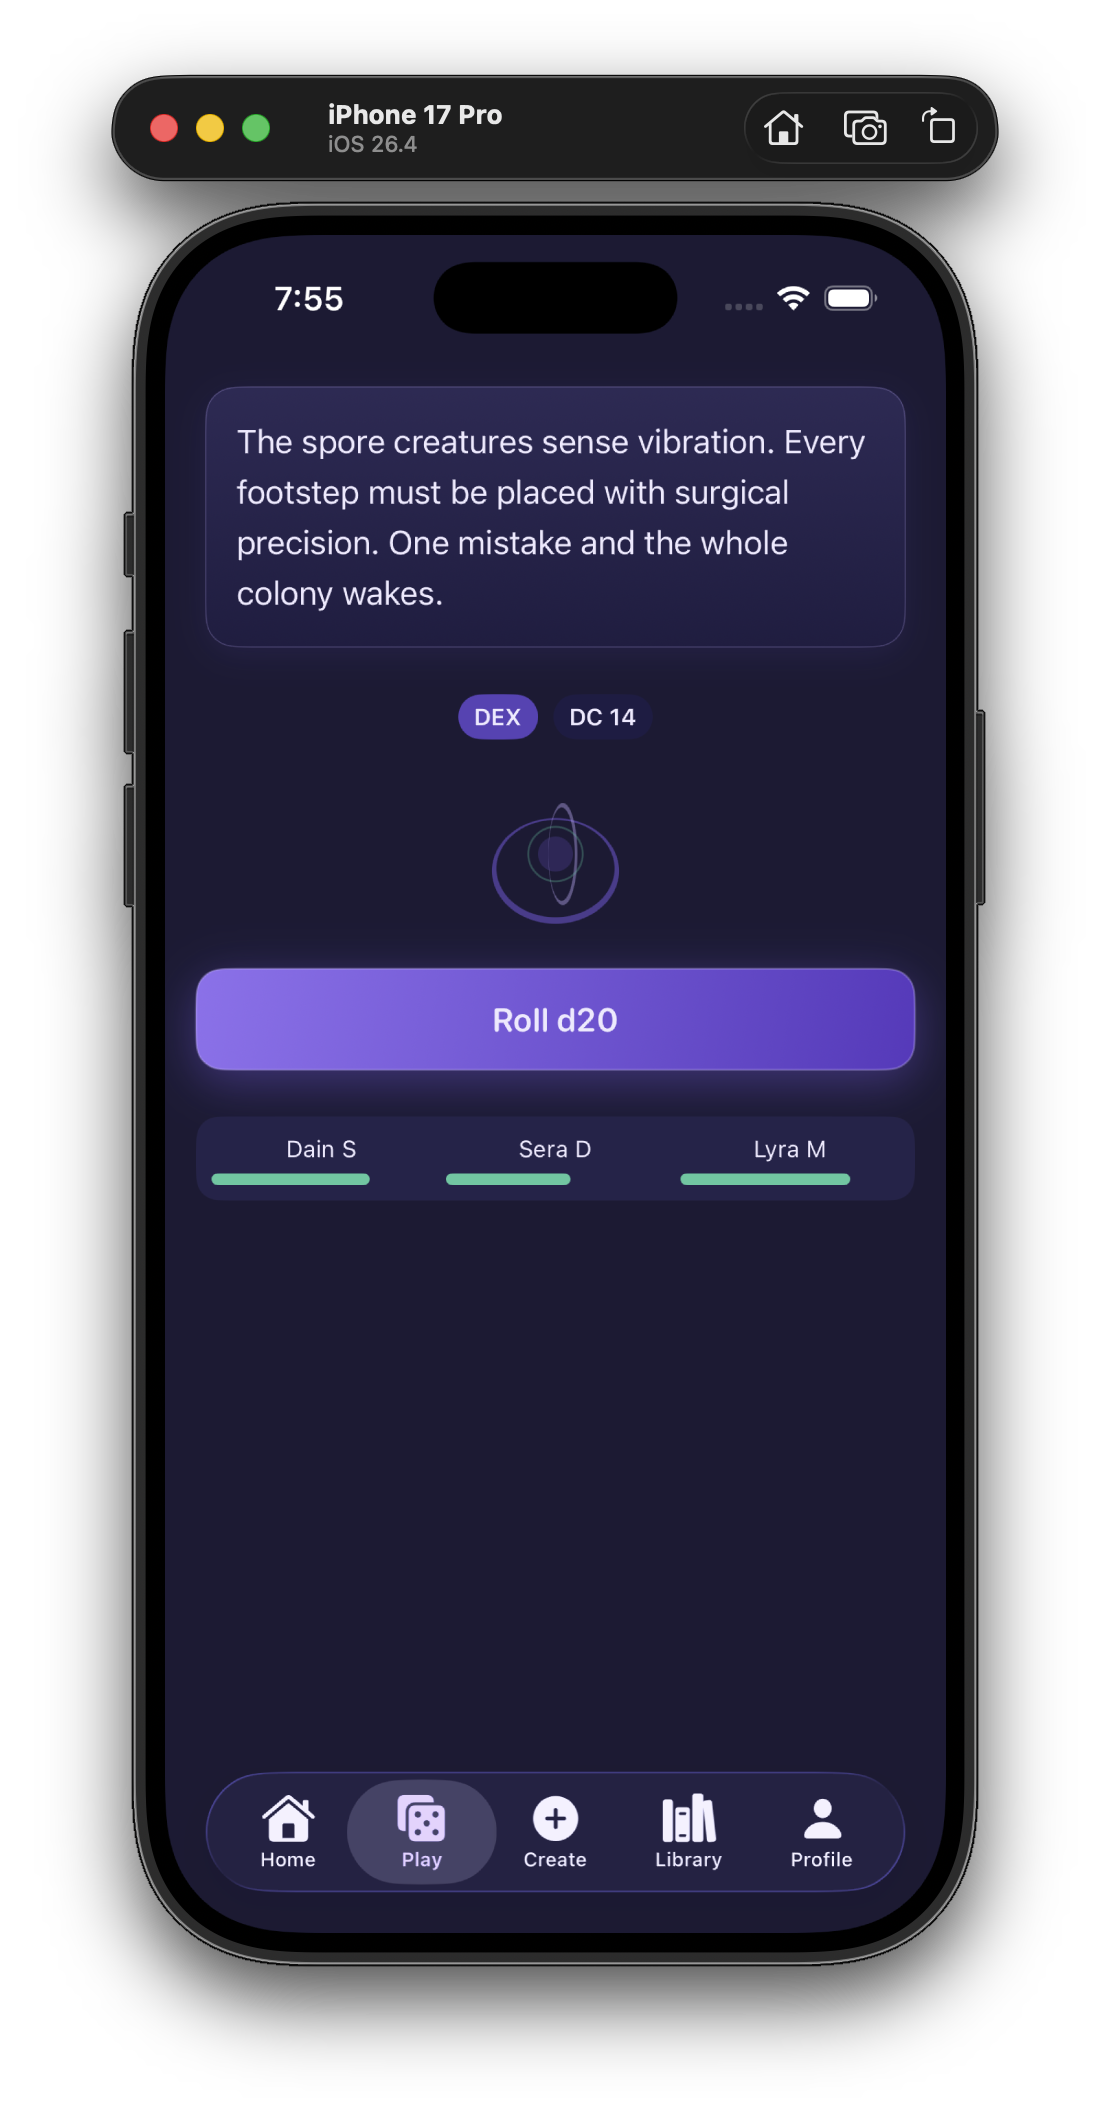
\includegraphics[width=\textwidth]{../images/9_8__play_d20_dice_roll.png}
    \caption{Skill Check}
  \end{subfigure}
  \hfill
  \begin{subfigure}[b]{0.3\textwidth}
    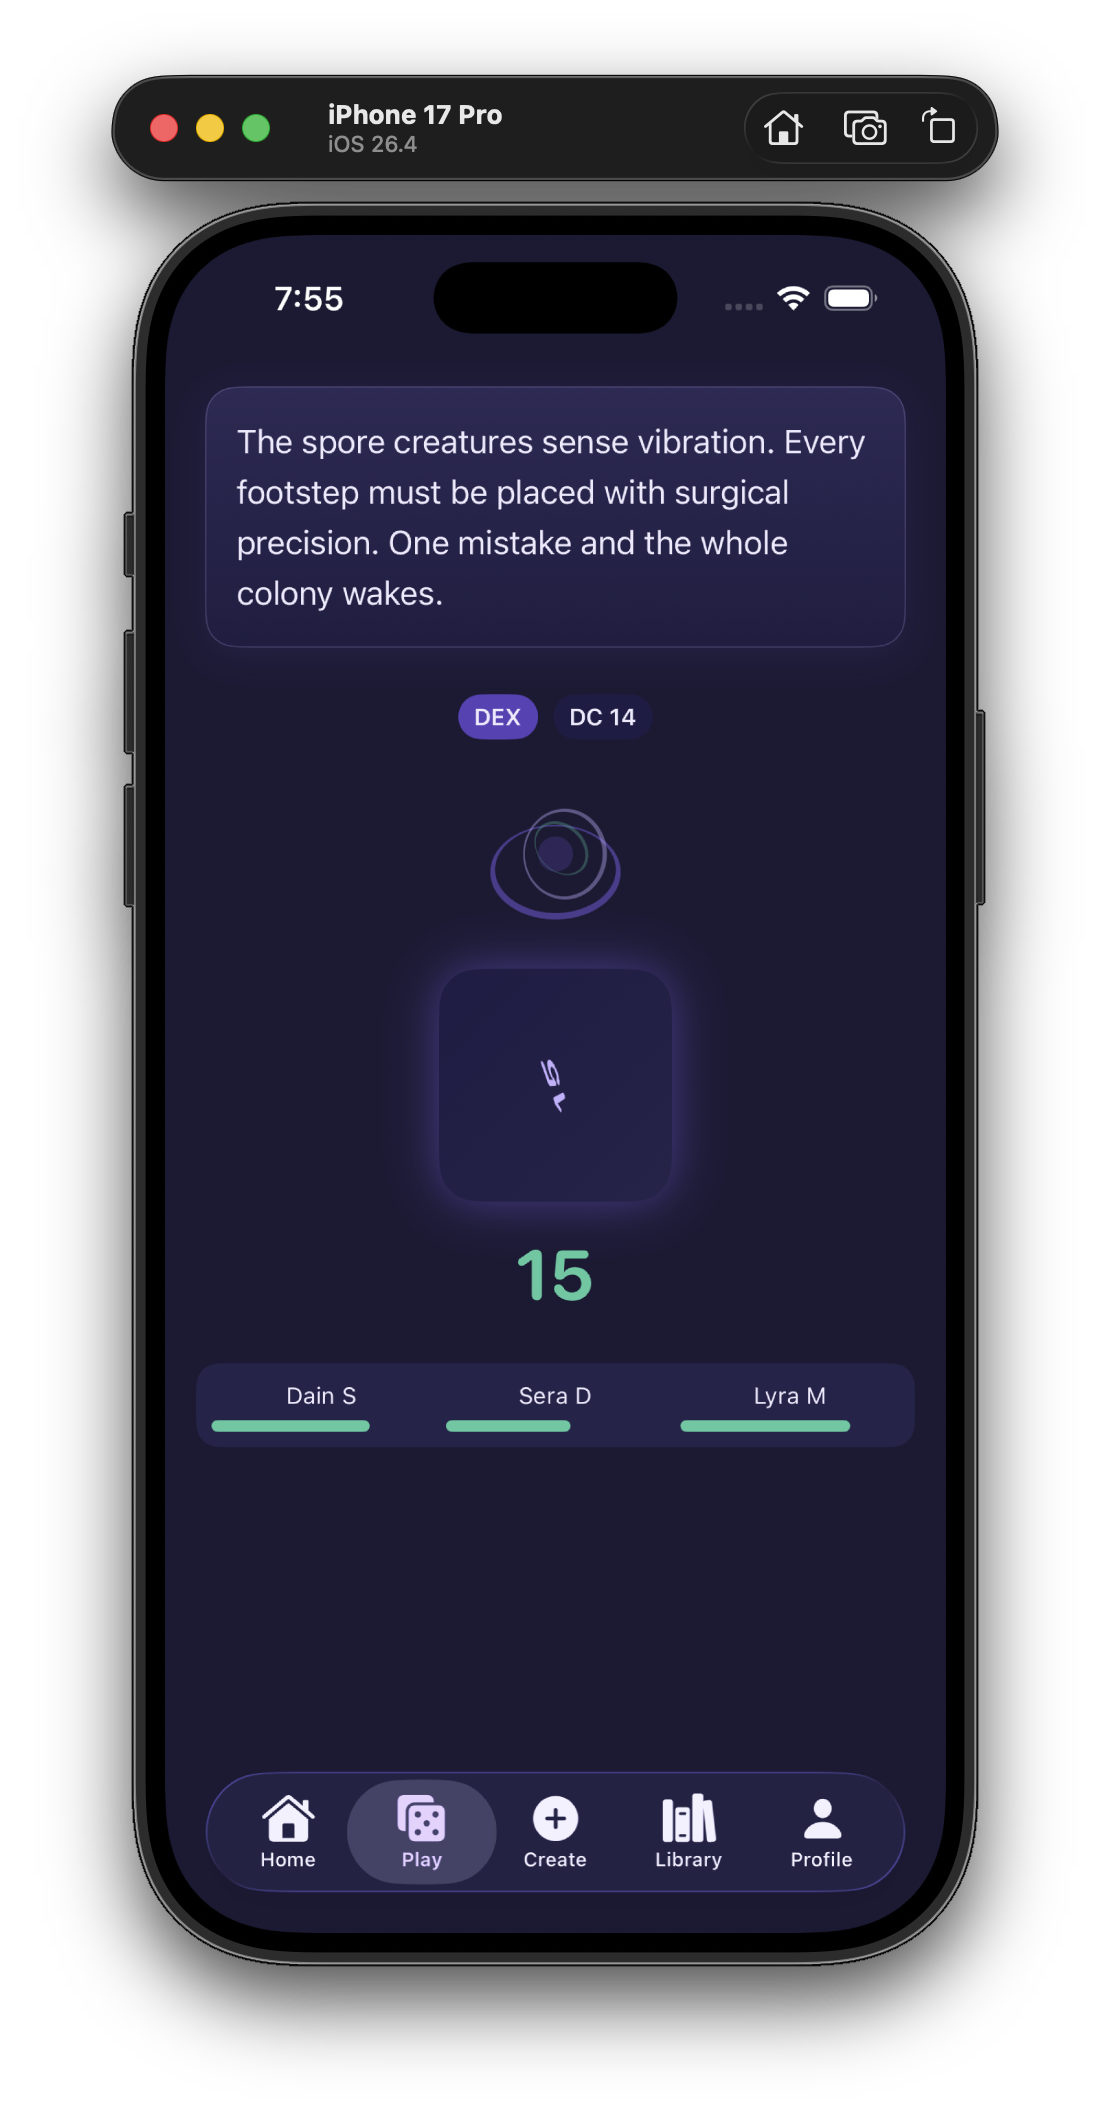
\includegraphics[width=\textwidth]{../images/9_9__play_d20_dice_roll_animation.png}
    \caption{Dice Roll Animation}
  \end{subfigure}
  \caption{Game Scene Engine — Combat and Skill Check}
\end{figure}

% ══════════════════════════════════════════════════════════════════════════════
\section{Architecture}

The app follows a strict MVVM architecture with a service-oriented domain layer, enforcing Swift~6 strict concurrency via \texttt{SWIFT\_DEFAULT\_ACTOR\_ISOLATION = MainActor}.

% ─────────────────────────────────────────────────────
\subsection{View Layer (SwiftUI)}

All screens live under \texttt{Views/} organised by feature:

{\small
\begin{verbatim}
Views/
├── Auth/        AuthView
├── Chat/        ChatView · ConversationView · MySessionsView
├── Effects/     DeathOverlay · particle effects
├── Game/        GameView · ExplorationView · CommunityStoriesView
├── Home/        HomeView · PostCardView · PostDetailView
│                NewsView · NewsCardView
├── Library/     LibraryView
├── Plus/        ActionHubView · CreateCharacterView · CreatePostView
│                CreateSkillView · CharacterBrowserView · SkillBrowserView
├── Profile/     ProfileView
├── SplashScreenView.swift
└── MainTabView.swift
\end{verbatim}
}

Views contain zero business logic. All state reads and mutations go through a bound ViewModel.

% ─────────────────────────────────────────────────────
\subsection{ViewModel Layer}

Each screen owns a dedicated \texttt{@MainActor final class \ldots{} : ObservableObject}:

\begin{center}
\begin{tabular}{>{\ttfamily\small}p{5.2cm} p{8.5cm}}
  \toprule
  \textbf{ViewModel} & \textbf{Responsibility} \\
  \midrule
  AuthViewModel             & Sign-in / Sign-up / Sign-out state \\
  GameViewModel             & Scene engine, combat loop, Gemini narration streaming, auto-save \\
  MultiplayerViewModel      & GameSession lobby, real-time turn synchronisation \\
  StoryBuilderViewModel     & Multi-step story authoring wizard and Firestore publish \\
  CommunityStoriesViewModel & Published user-story list \\
  ConversationViewModel     & Real-time chat message stream \\
  ChatViewModel             & Conversation list and connection-request management \\
  HomeViewModel             & Post feed, likes, emoji reactions, comments, replies \\
  NewsViewModel             & Tech and gaming news articles \\
  CreatePostViewModel       & Post form state and Cloudinary image upload \\
  CreateCharacterViewModel  & Character form validation and Firestore write \\
  CreateSkillViewModel      & Skill form validation and Firestore write \\
  CharacterBrowserViewModel & Character list with live search/filter \\
  SkillBrowserViewModel     & Skill list with live search/filter \\
  ProfileViewModel          & Analytics display, avatar upload, sign-out \\
  InventoryViewModel        & Player inventory item display \\
  \bottomrule
\end{tabular}
\end{center}

% ─────────────────────────────────────────────────────
\subsection{Service Layer}

\begin{center}
\begin{tabular}{>{\ttfamily\small}p{4cm} p{9.5cm}}
  \toprule
  \textbf{Service} & \textbf{Role} \\
  \midrule
  FirestoreService   & All Firestore reads, writes, and real-time snapshot listeners \\
  AuthService        & Firebase Auth session lifecycle, current UID access \\
  GeminiService      & Streamed narrative generation — Gemini Flash 2.0 SSE API \\
  CloudinaryService  & Image compression to 800\,px and upload; returns URL string \\
  NewsService        & Fetches tech/gaming news from external REST API \\
  HapticEngine       & Centralised \texttt{UIImpactFeedbackGenerator} calls \\
  SecretsManager     & Reads \texttt{Secrets.plist} for API keys at runtime \\
  \bottomrule
\end{tabular}
\end{center}

% ─────────────────────────────────────────────────────
\subsection{Game Engine Layer}

{\small
\begin{verbatim}
Game/
├── CampaignStoryProvider   — hard-coded 5-act, 25+ scene graph
├── UserStoryProvider       — runtime scene graph from UserStory model
├── SceneManager            — evaluates game-over / completion conditions
├── DefaultContent          — seeds 6 chars · 12 skills · 8 items
└── BotAI                   — role-based bot action selection per archetype
\end{verbatim}
}

\texttt{GameViewModel} depends only on the \texttt{StoryProvider} protocol, making both campaign and community-story runs use the identical code path.

% ─────────────────────────────────────────────────────
\subsection{Persistence}

\begin{center}
\begin{tabular}{ll}
  \toprule
  \textbf{Data} & \textbf{Store} \\
  \midrule
  Auth session              & Firebase Auth keychain \\
  Structured app data       & Firebase Firestore (offline persistence enabled) \\
  Images and portraits      & Cloudinary CDN \\
  API keys                  & Bundled \texttt{Secrets.plist} (git-ignored) \\
  Local UI state            & \texttt{@State} / \texttt{@StateObject} / \texttt{@AppStorage} \\
  \bottomrule
\end{tabular}
\end{center}

% ══════════════════════════════════════════════════════════════════════════════
\section{Project Structure}

{\small
\begin{verbatim}
storyweave/
├── storyweave/
│   ├── StoryWeaveApp.swift
│   ├── DesignSystem/
│   │   ├── Colors.swift  Components.swift
│   ├── Models/
│   │   ├── Character.swift  Skill.swift  Post.swift
│   │   ├── Comment.swift    Reaction.swift  UserProfile.swift
│   │   ├── GameState.swift  GameAnalytics.swift  GameSession.swift
│   │   ├── InventoryItem.swift  UserStory.swift  Connection.swift
│   │   ├── Conversation.swift  ChatMessage.swift  NewsArticle.swift
│   │   └── Enums.swift
│   ├── Services/
│   │   ├── AuthService.swift  FirestoreService.swift  GeminiService.swift
│   │   ├── CloudinaryService.swift  NewsService.swift
│   │   └── HapticEngine.swift  SecretsManager.swift
│   ├── ViewModels/   (16 view models — see Architecture)
│   ├── Views/        (feature folders  — see Architecture)
│   ├── Game/
│   │   ├── CampaignStoryProvider.swift  UserStoryProvider.swift
│   │   ├── SceneManager.swift  DefaultContent.swift
│   │   └── BotAI.swift
│   ├── PropertyWrappers/
│   ├── Assets.xcassets
│   ├── GoogleService-Info.plist
│   └── Secrets.plist
├── storyweave.xcodeproj/
├── docs/
└── images/
\end{verbatim}
}

% ══════════════════════════════════════════════════════════════════════════════
\section{Data Model / Entity Relationships}

% ── DIAGRAM PLACEHOLDER ───────────────────────────────────────────────────────
% Replace with: \includegraphics[width=\textwidth]{../images/diagram_er.png}
% (take a screenshot of the Mermaid ER diagram from Report.md)
\begin{figure}[H]
  \centering
  \includegraphics[max width=\textwidth,max height=0.85\textheight]{../images/_0__Database_Schema.png}
  \caption{Database Schema of StoryWeave App}
  \label{fig:er_diagram}
\end{figure}

The main entities and their relationships are summarised below:

\begin{itemize}[leftmargin=1.5em]
  \item \textbf{USER} owns a \textbf{GAME\_ANALYTICS} record, creates \textbf{CHARACTER}s and \textbf{SKILL}s, authors \textbf{POST}s and \textbf{USER\_STORY}s, and persists one \textbf{GAME\_STATE}.
  \item \textbf{GAME\_STATE} carries a collection of \textbf{INVENTORY\_ITEM}s.
  \item \textbf{CHARACTER} equips zero or more \textbf{SKILL}s.
  \item \textbf{POST} receives \textbf{COMMENT}s and \textbf{REACTION}s; a \textbf{COMMENT} can itself receive reply \textbf{COMMENT}s (one level deep).
  \item A \textbf{CONNECTION} between two users opens a \textbf{CONVERSATION}, which contains \textbf{CHAT\_MESSAGE}s.
  \item \textbf{USER\_STORY} contains up to 40 \textbf{USER\_STORY\_SCENE}s.
  \item \textbf{GAME\_SESSION} includes multiple \textbf{USER}s and \textbf{CHARACTER}s for multiplayer runs.
\end{itemize}

% ─────────────────────────────────────────────────────
\subsection{Firestore Collections}

\begin{center}
\footnotesize
\begin{tabular}{>{\ttfamily\raggedright}p{5cm} >{\raggedright}p{3.8cm} >{\raggedright\arraybackslash}p{5.5cm}}
  \toprule
  \textbf{Collection Path} & \textbf{Document Type} & \textbf{Notes} \\
  \midrule
  /users/\{uid\}                         & UserProfile + Analytics     & One document per authenticated user \\
  /characters/\{characterID\}            & Character                   & System + user-created; publicly readable \\
  /skills/\{skillID\}                    & Skill                       & System + user-created; publicly readable \\
  /posts/\{postID\}                      & Post                        & Social feed; publicly readable \\
  /posts/\{id\}/reactions/\{uid\}        & Reaction                    & One reaction per user per post \\
  /posts/\{id\}/\allowbreak comments/\{commentID\}   & Comment                     & Top-level and reply comments \\
  /gameSaves/\{uid\}                     & GameState                   & One save per user; offline persistence enabled \\
  /connections/\{pairID\}                & Connection                  & pairID = sorted UIDs joined by \texttt{\_} \\
  /conversations/\{pairID\}              & Conversation                & Mirrors connection pair \\
  /conversations/\{id\}/\allowbreak messages/\{id\}  & ChatMessage                 & Real-time snapshot listener \\
  /userStories/\{storyID\}               & UserStory (+ scenes)        & Community-published adventures \\
  /gameSessions/\{sessionID\}            & GameSession                 & Multiplayer with embedded GameState \\
  /meta/seed\_v1                         & sentinel                    & Written once; gates default content seeding \\
  \bottomrule
\end{tabular}
\normalsize
\end{center}

% ══════════════════════════════════════════════════════════════════════════════
\section{Use Case Diagram}

% ── DIAGRAM PLACEHOLDER ───────────────────────────────────────────────────────
% Replace with: \includegraphics[width=\textwidth]{../images/diagram_usecase.png}
% (take a screenshot of the Mermaid Use Case diagram from Report.md)
\begin{figure}[H]
  \centering
  
\includegraphics[max width=\textwidth,max height=0.85\textheight]{../images/_1__UseCase_Diagram.png}
  \caption{Use Case Diagram of StoryWeave App}
  \label{fig:usecase_diagram}
\end{figure}

The \textbf{Player} actor has access to all use cases: Authentication (Sign In, Sign Up, Reset Password), Community \& Social (Browse Feed, Create Post, React/Like/Comment, Read News), Direct Messaging (Connection requests, Chat), Library browsing, Create hub (Character, Skill, Post, Story), Game (Campaign, Community Story, Multiplayer, all scene types, Auto-Save), and Profile management.

A \textbf{Peer User} actor interacts with the social layer — approving or declining connection requests, exchanging messages, browsing the feed, and reacting to posts.

% ══════════════════════════════════════════════════════════════════════════════
\section{Activity Diagram}

% ── DIAGRAM PLACEHOLDER ───────────────────────────────────────────────────────
% Replace with: \includegraphics[width=\textwidth]{../images/diagram_activity.png}
% (take a screenshot of the Mermaid Activity diagram from Report.md)
\begin{figure}[H]
  \centering
  \includegraphics[max width=\textwidth,max height=0.85\textheight]{../images/_2__Activity_Diagram.png}
  \caption{Activity Diagram of StoryWeave App}
  \label{fig:activity_diagram}
\end{figure}

The activity flow begins at app launch. If the user is not authenticated, they are routed to Sign In or Create Account. Once authenticated, the Main Tab View is presented with five navigation destinations. Three parallel flows branch from there: the Community Flow (browse, post, react, message), the Create Flow (character, skill, post, or story creation), and the Game Flow. In the Game Flow, the player assembles a party, then enters the scene loop — Exploration scenes generate Gemini narration and branch on player choice; Combat and Skill Check scenes resolve via D20 rolls. The \texttt{GameState} is auto-saved to Firestore after every resolved scene. The loop continues until all party members are defeated (Game Over) or all acts are completed (Victory).

% ══════════════════════════════════════════════════════════════════════════════
\section{Team Contributions}

\begin{sloppypar}
\subsection*{Md.\ Shifat Hasan — \textit{Game Engine, Social Feed, \& News}}

Designed and implemented the entire game engine: the \texttt{StoryProvider} protocol and both concrete providers (\texttt{CampaignStoryProvider} and \texttt{UserStoryProvider}), \texttt{SceneManager}, \texttt{GameViewModel}, and \texttt{DefaultContent} seeding. Built the turn-based combat system including role-based bot AI (\texttt{BotAI}) for all six archetypes, D20 outcome resolution (\texttt{CombatOutcome}), skill-check branching, and party-death/game-over logic, with Basher providing supplementary support on gameplay integration. Integrated Google Gemini Flash~2.0 via Server-Sent Events into \texttt{GeminiService} returning an \texttt{AsyncThrowingStream<String, Error>} for typewriter-style streamed narration, resolving Swift~6 actor-boundary challenges. Implemented all SwiftUI-only visual effects: \texttt{rotation3DEffect} dice roll animation, hit flash overlays, death desaturation via \texttt{Canvas}, and level-up particle bursts using \texttt{TimelineView}. Also built the community social feed (\texttt{HomeViewModel}, \texttt{PostCardView}, \texttt{PostDetailView}, emoji reactions, threaded comments), the Create Post form, the tech/gaming news tab (\texttt{NewsService}, \texttt{NewsViewModel}, \texttt{NewsCardView}), and the multiplayer \texttt{GameSession} system.

\subsection*{Siam Basher — \textit{Direct Messaging, Character \& Skill Creation, Story Publish}}

Built the full direct-messaging system end-to-end: \texttt{Connection} and \texttt{Conversation} Firestore models, connection-request approval/decline flow, \texttt{ConversationViewModel} consuming a real-time Firestore \texttt{addSnapshotListener} bridged into an \texttt{AsyncStream}, \texttt{ChatView}, and \texttt{ConversationView} with colour-coded message bubbles. Implemented \texttt{CreateCharacterView} with archetype chip-row and five stat sliders, and \texttt{CreateSkillView} with stat and target-type chip rows, including their respective view models and Firestore write flows. Completed the final step of the community story builder wizard — the Review \& Publish screen (\texttt{StoryBuilderViewModel} publish flow, Firestore write of \texttt{UserStory}). Also provided supplementary support on game engine integration.

\subsection*{Afifa Sultana — \textit{Authentication, Profile + Library Tab \& Story Creation}}

Implemented all Firebase Auth flows: sign-in, account creation with display-name provisioning, password-reset email, and session-aware routing in \texttt{StoryWeaveApp}. Built the entire Profile tab: \texttt{ProfileViewModel}, Cloudinary-backed avatar upload with live circular preview, game-analytics tile grid (Combats Won/Lost, Acts Done, Heroes Lost, Skill Checks, Playtime), combat win-rate and skill-check accuracy progress indicators, inventory list via \texttt{InventoryViewModel}, and the Sign Out button. The Library character and skill browsers (\texttt{CharacterBrowserViewModel}, \texttt{SkillBrowserViewModel}, \texttt{LibraryView}). Implemented the first two steps of the community story builder wizard — Story Info (title and synopsis) and the Scenes editor (scene type, narration text, branching choices, combat and skill-check configuration per scene).
\end{sloppypar}

% ══════════════════════════════════════════════════════════════════════════════
\section{Discussion}

\begin{sloppypar}
A significant technical challenge was integrating Google Gemini's SSE streaming API within Swift~6's strict actor isolation. \texttt{GeminiService} returns an \texttt{AsyncThrowingStream<String, Error>} from a \texttt{nonisolated} method, and \texttt{GameViewModel} — pinned to \texttt{@MainActor} — must progressively append tokens to \texttt{@Published var narration} without data races. The solution was to open a detached \texttt{Task} inside the ViewModel that consumes the stream with \texttt{for try await}, writing each chunk to \texttt{@MainActor} state, and cancels via a stored \texttt{Task} reference on every scene transition.

A second challenge was designing a story engine that handles both the hard-coded five-act campaign and arbitrary user-authored adventures through the same code path. Introducing a \texttt{StoryProvider} protocol implemented by \texttt{CampaignStoryProvider} and \texttt{UserStoryProvider} allowed \texttt{GameViewModel} to remain provider-agnostic. Swapping the provider at game-start is sufficient to run any story type with zero branching logic in the engine itself.

A third challenge involved bridging Firestore's callback-based snapshot listeners into the Swift async/await world for real-time chat. Wrapping each \texttt{addSnapshotListener} call in an \texttt{AsyncStream \{ continuation in \ldots{} \}} inside \texttt{FirestoreService} exposed a typed async sequence that \texttt{ConversationViewModel} could consume with \texttt{for await} on the \texttt{@MainActor}, satisfying Swift~6 \texttt{Sendable} requirements while delivering sub-second message delivery.

Finally, building all animations — dice rolls, combat screen shakes, death dissolves, level-up glows — entirely in SwiftUI without external assets required creative use of \texttt{TimelineView}, \texttt{Canvas}, \texttt{GeometryEffect}, and \texttt{rotation3DEffect}. Confining particle-system draw calls to \texttt{TimelineView} with an \texttt{.animation} schedule prevented layout passes on every frame tick and maintained a smooth 60\,fps throughout combat sequences.
\end{sloppypar}

% ══════════════════════════════════════════════════════════════════════════════
\section{Conclusion}

\begin{sloppypar}
StoryWeave delivers a complete, production-quality iOS experience combining a five-act AI-narrated RPG with a real-time social community. Swift~6 strict concurrency, MVVM architecture, and the \texttt{StoryProvider} protocol made the game engine fully decoupled from both the campaign content and the social layer, enabling all three to evolve independently. Firebase Firestore's offline persistence means game saves survive network interruptions, while Gemini Flash~2.0 streaming keeps narrative latency imperceptible. The project provided hands-on experience in streaming API integration, protocol-driven game-engine design, actor-safe real-time data pipelines, and building complex animations purely from SwiftUI primitives — demonstrating that modern iOS frameworks are capable of powering immersive, multi-user interactive experiences without a single external asset file.
\end{sloppypar}

% ══════════════════════════════════════════════════════════════════════════════
\section*{References}
\addcontentsline{toc}{section}{References}

\begin{sloppypar}
\begin{enumerate}[leftmargin=2em]
  \item Apple Inc. \textit{SwiftUI Documentation}. \url{https://developer.apple.com/documentation/swiftui}
  \item Apple Inc. \textit{Swift Concurrency}. \url{https://developer.apple.com/documentation/swift/concurrency}
  \item Google. \textit{Firebase iOS SDK Setup}. \url{https://firebase.google.com/docs/ios/setup}
  \item Google. \textit{Firebase Firestore}. \url{https://firebase.google.com/docs/firestore}
  \item Google. \textit{Gemini API — Streaming}. \url{https://ai.google.dev/gemini-api/docs/text-generation#streaming}
  \item Cloudinary. \textit{iOS Integration Guide}. \url{https://cloudinary.com/documentation/ios_integration}
  \item Mermaid. \textit{Diagramming Language}. \url{https://mermaid.js.org}
\end{enumerate}
\end{sloppypar}

% ─────────────────────────────────────────────────────────────────────────────
\end{document}
